\documentclass[reqno]{amsart}
\usepackage{amscd, amssymb, amsmath, amsthm}
\usepackage{graphicx}
\usepackage[colorlinks=true,linkcolor=blue]{hyperref}
\usepackage[utf8]{inputenc}
\usepackage[T1]{fontenc}
\usepackage{textcomp}
\usepackage{babel}
%% for identity function 1:
\usepackage{bbm}
%%For category theory diagrams:
\usepackage{tikz-cd}

\usepackage[backend=biber]{biblatex}
\addbibresource{notes.bib}

\setlength\parindent{0pt}

\pdfsuppresswarningpagegroup=1

\newtheorem{theorem}{Theorem}[section]
\newtheorem{lemma}[theorem]{Lemma}
\newtheorem{proposition}[theorem]{Proposition}
\newtheorem{corollary}[theorem]{Corollary}
\newtheorem{conjecture}[theorem]{Conjecture}

\theoremstyle{definition}
\newtheorem{definition}[theorem]{Definition}
\newtheorem{example}[theorem]{Example}
\newtheorem{exercise}[theorem]{Exercise}
\newtheorem{problem}[theorem]{Problem}
\newtheorem{question}[theorem]{Question}

\theoremstyle{remark}
\newtheorem*{remark}{Remark}
\newtheorem*{note}{Note}
\newtheorem*{solution}{Solution}
\newtheorem*{slogan}{Slogan}
\newtheorem*{assertion}{Assertion}



%Inequalities
\newcommand{\cycsum}{\sum_{\mathrm{cyc}}}
\newcommand{\symsum}{\sum_{\mathrm{sym}}}
\newcommand{\cycprod}{\prod_{\mathrm{cyc}}}
\newcommand{\symprod}{\prod_{\mathrm{sym}}}

%Linear Algebra

\DeclareMathOperator{\Span}{span}
\DeclareMathOperator{\im}{im}
\DeclareMathOperator{\diag}{diag}
\DeclareMathOperator{\Ker}{Ker}
\DeclareMathOperator{\ob}{ob}
\DeclareMathOperator{\Hom}{Hom}
\DeclareMathOperator{\Mor}{Mor}
\DeclareMathOperator{\sk}{sk}
\DeclareMathOperator{\Vect}{Vect}
\DeclareMathOperator{\Set}{Set}
\DeclareMathOperator{\Group}{Group}
\DeclareMathOperator{\Ring}{Ring}
\DeclareMathOperator{\Ab}{Ab}
\DeclareMathOperator{\Top}{Top}
\DeclareMathOperator{\hTop}{hTop}
\DeclareMathOperator{\Htpy}{Htpy}
\DeclareMathOperator{\Cat}{Cat}
\DeclareMathOperator{\CAT}{CAT}
\DeclareMathOperator{\Cone}{Cone}
\DeclareMathOperator{\dom}{dom}
\DeclareMathOperator{\cod}{cod}
\DeclareMathOperator{\Aut}{Aut}
\DeclareMathOperator{\Mat}{Mat}
\DeclareMathOperator{\Fin}{Fin}
\DeclareMathOperator{\rel}{rel}
\DeclareMathOperator{\Int}{int}
\DeclareMathOperator{\sgn}{sgn}
\DeclareMathOperator{\Homeo}{Homeo}
\DeclareMathOperator{\SHomeo}{SHomeo}
\DeclareMathOperator{\PSL}{PSL}
\DeclareMathOperator{\Bil}{Bil}
\DeclareMathOperator{\Sym}{Sym}
\DeclareMathOperator{\Skew}{Skew}
\DeclareMathOperator{\Alt}{Alt}
\DeclareMathOperator{\Quad}{Quad}
\DeclareMathOperator{\Sin}{Sin}
\DeclareMathOperator{\Supp}{Supp}
\DeclareMathOperator{\Char}{char}
\DeclareMathOperator{\Teich}{Teich}
\DeclareMathOperator{\GL}{GL}
\DeclareMathOperator{\tr}{tr}
\DeclareMathOperator{\codim}{codim}
\DeclareMathOperator{\coker}{coker}
\DeclareMathOperator{\corank}{corank}
\DeclareMathOperator{\rank}{rank}
\DeclareMathOperator{\Diff}{Diff}
\DeclareMathOperator{\Bun}{Bun}
\DeclareMathOperator{\Sm}{Sm}
\DeclareMathOperator{\Fr}{Fr}
\DeclareMathOperator{\Cob}{Cob}
\DeclareMathOperator{\Ext}{Ext}





%Row operations
\newcommand{\elem}[1]{% elementary operations
\xrightarrow{\substack{#1}}%
}

\newcommand{\lelem}[1]{% elementary operations (left alignment)
\xrightarrow{\begin{subarray}{l}#1\end{subarray}}%
}

%SS
\DeclareMathOperator{\supp}{supp}
\DeclareMathOperator{\Var}{Var}

%NT
\DeclareMathOperator{\ord}{ord}

%Alg
\DeclareMathOperator{\Rad}{Rad}
\DeclareMathOperator{\Jac}{Jac}

%Misc
\newcommand{\SL}{{\mathrm{SL}}}
\newcommand{\mobgp}{{\mathrm{PSL}_2(\mathbb{C})}}
\newcommand{\id}{{\mathrm{id}}}
\newcommand{\MCG}{{\mathrm{MCG}}}
\newcommand{\PMCG}{{\mathrm{PMCG}}}
\newcommand{\SMCG}{{\mathrm{SMCG}}}
\newcommand{\ud}{{\mathrm{d}}}
\newcommand{\Vol}{{\mathrm{Vol}}}
\newcommand{\Area}{{\mathrm{Area}}}
\newcommand{\diam}{{\mathrm{diam}}}
\newcommand{\End}{{\mathrm{End}}}


\newcommand{\reg}{{\mathtt{reg}}}
\newcommand{\geo}{{\mathtt{geo}}}

\newcommand{\tori}{{\mathcal{T}}}
\newcommand{\cpn}{{\mathtt{c}}}
\newcommand{\pat}{{\mathtt{p}}}

\let\Cap\undefined
\newcommand{\Cap}{{\mathcal{C}}ap}
\newcommand{\Push}{{\mathcal{P}}ush}
\newcommand{\Forget}{{\mathcal{F}}orget}

\tikzset{
    labl/.style={anchor=south, rotate=135, inner sep=.5mm}
}

\title{Geometric Topology}
\author{Jonas Trepiakas}
\date{}


\begin{document}
\maketitle

\tableofcontents


\section{Introduction}

My primary two reference books for differential geometry
for these notes will be \cite{KMS} and \cite{LeeSM}.


\section{Continuous maps}


    \begin{definition}[]
        For a continuous map $f \colon M \to N$ between 
        topological manifolds,
        \begin{itemize}
            \item $f$ is called
                an immersion if
                locally at each point of $M$,
                it is of the form
                $\mathbb{R}^{m} \to \mathbb{R}^{n}$ 
                sending $x \mapsto \left( x,0 \right) $.
            \item $f$ is an embedding if it is
                an immersion, injective and induces a homeomorphism
                with
                its image.
            \item $f$ is a submersion if it is locally
                of the form to
                $\left( x,y \right) \mapsto x$.
        \end{itemize}
    \end{definition}

    \begin{definition}[Bundle as defined by
        Robert (is this supposed to be a fiber bundle?)]
        If 
        $f \colon M \to N$ is a continuous
        map between topological manifolds, then
        $f$ is called a bundle if it is locally
        on $N$ of the form
        $X \times V \stackrel{\pi_2}{\to } V$.
        That is, there
        exist charts, in which
        $f$ takes the form of a projection.
    \end{definition}

\section{Smooth Manifolds}


\begin{proposition}[Manifolds are Locally Compact]
    Every topological manifold is
    locally compact.
\end{proposition}

\begin{definition}[]
    Let $M$ be a topological space. A collection
    $\mathcal{X}$ of subsets of $M$ is said to be
    \textit{locally finite} if each point of $M$ has
    a neighborhood that intersects at most finitely many
    of the sets in $\mathcal{X}$. Given a cover
    $\mathcal{U}$ of $M$, we say that another cover
    $\mathcal{V}$ is a \textit{refinement of $\mathcal{U}$ }
    if for each $V \in \mathcal{V}$, there exists
    some $U \in \mathcal{U}$ such that
    $V \subset U$. 
\end{definition}

\begin{definition}[Paracompactness]
    We say that a topological space $M$ is 
    \textit{paracompact} if every open cover of $M$ admits
    an open, locally finite refinement.
\end{definition}

\begin{theorem}[Manifolds are Paracompact]
    Every topological manifold is paracompact.
    In fact, given a topological manifold $M$, an
    open cover $\mathcal{X}$ of $M$ and any basis
    $\mathcal{B}$ for the topology of $M$, there
    exists a countable, locally finite open
    refinement of $\mathcal{X}$ consisting of elements
    of $\mathcal{B}$.
\end{theorem}

\begin{theorem}[]
    The fundamental group of a topological manifold is
    countable.
\end{theorem}


\begin{definition}[]
    We say a set $B \subset M$ is a \textit{regular coordinate
    ball} if there is a smooth coordinate ball
    $B' \supset \overline{B}$ and a smooth coordinate
    map $\varphi \colon B' \to \mathbb{R}^{n}$ such that
    for some positive real numbers $r < r'$,
    \[
    \varphi (B) = B_r (0), \quad
    \varphi \left( \overline{B} \right) 
    = \overline{B}_r (0), \quad \text{and} \quad
    \varphi (B') = B_{r'}(0).
    \] 
\end{definition}


\begin{proposition}[]\label{Mfds-regular-coordinate-balls}
    Every smooth manifold has a countable basis of
    regular coordinate balls.
\end{proposition}


\begin{definition}[]
    A subset of a topological space $X$ is said to
    be \textit{precompact in $X$} if its closure in
    $X$ is compact.
\end{definition}

\begin{exercise}[]
    For a Hausdorff space $X$, the following are equivalent
    \begin{enumerate}
        \item $X$ is locally compact.
        \item Each point of $X$ has a precompact neighborhood.
        \item $X$ has a basis of precompact open subsets.
    \end{enumerate}
\end{exercise}


\begin{definition}[]
    A sequence 
    $\left( K_i \right)_{i \in \mathbb{N} }$ of compact subsets
    of a topological space $X$ is called an
    \textit{exhaustion of $X$ by compact sets} if
    $X = \bigcup_{i}  K_i$ and
    $K_i \subset \int K_{i+1}$ for each $i$.
\end{definition}

\begin{proposition}[]
    A second-countable, locally compact
    Hausdorff space admits an exhaustion by compact
    sets.
\end{proposition}


\begin{lemma}[]\label{Smooth-Mfds-Metrizable}
    \cite[Lemma 5.9]{GG}
    Any smooth manifold is metrizable.
\end{lemma}


\section{Smooth Maps}


\subsection{A couple of nice formula}

\begin{lemma}[Change of coordinates on tangent basis]
    Suppose
    $\left( U, \varphi  \right) ,
    \left( V,\psi  \right) $ are smooth charts
    on a smooth manifold $M$ and $p \in U \cap V$.
    Let $\left( x^{i} \right) , \left( \tilde{x}^{i} \right) $ 
    be the coordinate functions for $\varphi $ and $\psi $,
    respectively. 
    We can write
    \[
    \psi \circ \varphi^{-1} (x) =
    \left( \tilde{x}^{1}(x),\ldots,
    \tilde{x}^{n}(x) \right) .
    \] 
    Now
    \[
    \frac{\partial}{\partial x^{i}}|_{p}
    = \frac{\partial \tilde{x}^{j}}{\partial x^{i}}(p)
    \frac{\partial}{\partial \tilde{x}^{j}}|_p
    \] 
    where $\tilde{p} = \varphi (p)$ and we are using
    Einstein summation.
\end{lemma}



There are very few strong things that we can at this point
say about general smooth maps. This section will cover
the big tools.\\

The most important construction on manifolds is
that they posses partitions of unity.

\begin{definition}[Partition of unity]
    Suppose $M$ is a topological space and let
    $\mathcal{X} = \left( X_{\alpha} \right)_{\alpha \in A}$ 
    be an arbitrary open cover
    of $M$. A \textit{partition of unity
    subordinate to $\mathcal{X}$} is
    an indexed family
    $\left( \psi_{\alpha} \right)_{\alpha \in A}$ of 
    continuous functions
    $\psi_{\alpha} \colon M \to \mathbb{R}$ with the
    following properties:
    \begin{enumerate}
        \item $0 \le \psi_{\alpha}(x) \le 1$ for all
            $\alpha \in A$ and $x \in M$ 
        \item $\supp \psi_{\alpha} \subset X_{\alpha}$
            for all $\alpha \in A$ 
        \item The family of supports
            $\left( \supp \psi_{\alpha} \right)_{\alpha
            \in A}$ is locally finite (or we say
            that the partition of unity or the space
            is locally finite), meaning that
            every point has a neighborhood that intersects
            $\supp \psi_{\alpha}$ for only finitely many
            values of $\alpha$.
        \item $\sum_{\alpha \in A}\psi_{\alpha}(x) = 1$
            for all $x \in M$.
    \end{enumerate}
    When $M$ is a smooth manifold, a
    \textit{smooth partition of unity} is one for which
    each $\psi_{\alpha}$ is smooth.
\end{definition}

\begin{theorem}[Existence of Partitions of Unity]
    Suppose $M$ is a smooth manifold with
    or without boundary, and
    $\mathcal{X} = \left( X_{\alpha} \right)_{\alpha \in A}$ 
    is a cover of $M$. Then there
    exists a smooth partition of unity subordinate
    to $\mathcal{X}$.
\end{theorem}

\begin{theorem}[Existence of Partitions of Unity for
    Paracompact Spaces]
    If $X$ is a paracompact space, then for every
    open cover, there exists a partition of
    unity subordinate to the covering.
\end{theorem}


\begin{definition}[Bump functions]
    If $M$ is a topological space, $A \subset M$ 
    a closed subset, and
    $U \subset M$ an open subset containing $A$, a
    continuous function
    $\psi \colon M \to \mathbb{R}$ is called a
    \textit{bump function for $A$ supported
    in $U$} if $0 \le \psi  \le 1$ on
    $M$, $\psi \equiv 1$ on $A$, and $\supp \psi \subset U$.
\end{definition}

\begin{proposition}[Existence of Smooth Bump Functions]
    Let $M$ be a smooth manifold. For any closed
    subset $A \subset M$ and any open subset
    $U$ containing $A$, there exists a smooth bump function
    for $A$ supported in $U$.
\end{proposition}

\begin{note}
    The existence of bump functions give us a
    direct insight into just how different
    geometry is from complex analysis. 
    In complex analysis, knowing a function in a
    small region determines it uniquely, while
    the very existence of smooth bump functions
    for smooth manifolds tells us
    that functions cannot be determined from local
    behavior.
    In fact, smooth partitions of unity give
    us a way to glue function patches together
    on the different parts of the manifold to give
    arbitrarily complicated functions.
    This makes the study of geometry very broad and flexible compared
    to complex analysis, for example.
\end{note}


Another strong property of general smooth maps is
encapsulated in Sard's theorem:

\begin{theorem}[Sard's theorem]
    The set of critical values of a smooth
    map between manifolds has Lebesgue measure zero.
\end{theorem}


\subsubsection{Submersions, Immersions and Embeddings}

\begin{theorem}[]\cite[Thm 2.8]{GG}
    Let $X$ and $Y$ be $C^{k}$-manifolds of
    dimensions $n$ and $m$, respectively, with $n > m$. Let
    $\varphi  \colon X \to Y$ be a $C^{k}$-map. Then
    \begin{enumerate}
        \item If $\varphi $ is a submersion, then $\varphi $ is
            an open map.
        \item Let $Z$ be a submanifold of $Y$. If
            $\varphi $ is a submersion at each point
            in $\varphi^{-1}(Z)$, then
            $\varphi^{-1}(Z)$ is a $C^{k}$-submanifold of
            $X$ with $\codim \varphi^{-1}(Z) = 
            \codim Z$.
    \end{enumerate}
\end{theorem}

\begin{corollary}[Regular Value Theorem]\label{Regular-Value-Theorem}
    If $q$ is a regular value of a smooth map
    $f \colon M^{n+k} \to N^{n}$, then
    $f^{-1}(q)$ is a smooth submanifold of $M$ of codimension
    $n$.
\end{corollary}



\begin{definition}[Locally Trivial Fibration/Bundle]
    A locally trivial fibration (following \cite{JB}) or
    a Bundle (following Robert), is
    a map $f \colon E \to M$ between smooth manifolds
    such that at each point $p \in M$, there exists
    a neighborhood $U$ of $p$ such that there
    exists a diffeomorphism
    $\varphi \colon U \times F \cong f^{-1}(U)$ for
    $F = f^{-1}(p)$, making the following diagram
    commute:
    \begin{equation*}
    \begin{tikzcd}
        U \ar[dr, "\pi_1"] \times F \ar[rr, "\varphi "] 
        & & f^{-1}(U) \ar[dl, "f|_{f^{-1}(U)}"] \\
        & U &
    \end{tikzcd}
    \end{equation*}
    
\end{definition}



\begin{theorem}[Fibration Theorem of Ehresmann]
    Let $f \colon E \to M$ be a proper
    submersion of smooth manifolds. Then
    $f$ is a locally trivial fibration.
\end{theorem}



\newpage

\section{Transversality and Function Spaces}

For this section, we will closely be following
\cite{GG}.


\begin{definition}[]
    Given maps
    \begin{equation*}
    \begin{tikzcd}
        & Y \ar[d,"g"] \\
        X \ar[r, "f"] & Z
    \end{tikzcd}
    \end{equation*}
    we say that $f$ is transverse to $g$, denoted
    $f \pitchfork g$ if for every
    $p \in X$ and every $q \in Y$ such that
    $f(p) = g(y)$, we have
    \[
        \left( TX \right)_p \oplus \left( TY \right)_{q}
        \twoheadrightarrow \left( TZ \right)_{f(p)}
    \] 
\end{definition}


\subsection{Jet Bundles}

\begin{definition}[]
   Let $X,Y$ be smooth manifolds and $p \in X$. 
   Suppose $f,g \colon X \to Y$ are smooth
   with $f(p) = g(p) = q$.
   \begin{enumerate}
       \item We that $f$ has \textit{first order contact
           with $g$ at $p$ } if $\left( df \right)_p
           = \left( dg \right)_p \colon
           T_p X \to T_q Y$ .
       \item We say that \textit{$f$ has $k$ th order
           contact with $g$ at $p$} if
           $\left( df \right) \colon
           TX \to TY$ has $\left( k-1 \right) $ st
           order contact with $\left( dg \right) $ at
           every point in $T_p X$. This is written
           as $f \sim_k g$ at $p$.
       \item Let $J^{k}(X,Y)_{p,q}$ denote the
           set of equivalence classes under
           " $\sim_k$ at $p$ " of smooth maps
           $f \colon X \to Y$ where
           $f(p) = q$.
       \item Define $J^{k}(X,Y) :=
           \bigcup_{\left( p,q \right) \in X \times Y} 
           J^{k}(X,Y)_{p,q}$. An element
           $\sigma \in J^{k}(X,Y)$ is called a 
           \textit{$k$-jet of mappings (or just a $k$-jet)
           from $X$ to $Y$}.
       \item Let $\sigma$ be a $k$-jet. Then
           for some $\left( p,q \right) \in X \times Y$,
           $\sigma \in J^{k}(X,Y)_{p,q}$. Then
           $p$ is called the source of $\sigma$ and
           $q$ is called the target of $\sigma$. The
           mapping $\alpha \colon J^{k}(X,Y) \to X$ 
           given by $\sigma \mapsto \text{source of } \sigma$ 
           is called the source map and the mapping
           $\beta \colon J^{k}(X,Y) \to Y$ given by
           $\sigma \mapsto \text{target of }\sigma$ is called
           the target map.
   \end{enumerate}
\end{definition}

\begin{definition}[$k$-jet or the $k$-prolongation of a map]
    For a smooth map
    $f \colon X \to Y$, there is a canonically defined map
    $j^{k}f \colon X \to J^{k}(X,Y)$ called the
    $k$-jet of $f$ defined by
    $j^{k}f(p) = \left[ f, p \right] $, the
    equivalence class of $f$ in
    $J^{k}(X,Y)_{p, f(p)}$, for every
    $p \in X$.
\end{definition}

\begin{lemma}[]\label{Jets-Taylor-Series}
    Let $U \subset \mathbb{R}^{n}$ be open and
    $p \in U$. Let $f,g \colon U \to \mathbb{R}^{m}$ be
    smooth. Then
    $f \sim_k g$ at $p$ if and only if
    \[
    \frac{\partial^{\left| \alpha \right| } f_i}{\partial
    x^{\alpha}}(p) = \frac{\partial^{\left| \alpha \right| }
g_i}{\partial x^{\alpha}}(p)
    \] 
    for every multi-index $\alpha$ with
    $\left| \alpha \right| \le k$ and
    $1\le y \le m$ where $f_i$ and $g_i$ are the
    coordinate functions determined by
    $f$ and $g$, respectively, and $x_1, \ldots, x_n$ 
    are coordinates on $U$.
\end{lemma}



\begin{lemma}[]
    Let $U \subset \mathbb{R}^{n}$ and
    $V \subset \mathbb{R}^{m}$ be open. 
    Let $f_1,f_2 \colon U \to V$ and
    $g_1,g_2 \colon V \to \mathbb{R}^{l}$ be smooth.
    Let $p \in U$.
    If $f_1 \sim_k f_2$ at $p$ and
    $g_1 \sim_k g_2$ at $q = f_1(p) = f_2(p)$, then
    $g_1 \circ f_1 \sim_k g_2 \circ f_2$ at $p$.
\end{lemma}

\begin{proof}
    We proceed by induction. First, we show the case
    when $k = 1$. In this case, the statement is precisely that
    \[
    d \left( g_1 \circ f_1 \right)_p = d\left( g_2
    \circ f_2\right)_p
    \] 
    for all $p \in U$.
    But this is true by the chain rule (Lemma
    \ref{Chain-Rule}):
    \[
    d\left( g_1 \circ f_1 \right)_p =
    \left( dg_1 \right)_q \left( df_1 \right)_p
    = \left( dg_2 \right)_q \left( df_2 \right)_p
    = d\left( g_2 \circ f_2 \right)_p.
    \] 
    Suppose now the statement is
    true for $k-1$.
    Then since
    $(df_1) \sim_{k-1} \left( df_2 \right) $ at
    $p$ and $\left( dg_1 \right) \sim_{k-1} \left( dg_2 \right) $ 
    at $q = f_1(p) = f_2(p)$, we have by
    induction that
    \[
        \left( dg_1  \right) \circ \left( df_1 \right) 
        \sim_{k-1} \left( dg_2 \right) \circ
        \left( df_2 \right) \quad
        \forall \left( p,v \right) \in \left\{ p \right\} \times 
        \mathbb{R}^{n}
    \] 
    which by the chain rule is precisely saying that
    \[
    d\left( g_1 \circ f_1 \right) \sim_{k-1}
    d\left( g_2 \circ f_2 \right) 
    \] 
    for all $(p,v) \in \left\{ p \right\} \times \mathbb{R}^{n}$.
    But this is precisely the definition of
    $g_1 \circ f_1 \sim_k g_2 \circ f_2$ at
    $p$.

\end{proof}

\begin{definition}[]
    Let $X,Y,Z,W$ be smooth manifolds.
    \begin{enumerate}
        \item Let $h \colon Y \to Z$ be smooth.a
            Then $h$ induces a map
            $h_* \colon J^{k}(X,Y) \to 
            J^{k}(X,Z)$ as follows:
            if $\left[ f,p \right]  \in J^{k}(X,Y)_{p,q}$, then
            $h_* \left[ f,p \right] =
            \left[ h \circ f, p \right] 
            \in J^{k}\left( X,Z \right)_{p,h(q)}$.
        \item If $a \colon Z \to W$ is smooth, then
            $\left( a \circ h \right)_{*}
            = a_* \circ h_*$ and
            $\left( \id_Y \right)_* = 
            \id_{J^{k}(X,Y)}$. So if
            $h$ is a diffeomorphism, then
            $h_*$ is a bijection.
        \item Let $g \colon Z \to X$ be a smooth
            diffeomorphism. Then
            $g$ induces a map
            $g^{*} \colon J^{k}(X,Y) \to 
            J^{k}(Z,Y)$ by
            $g^{*}\left[ f,p \right] =
            \left[ f \circ g, g^{-1}(p) \right] 
            \in J^k (Z,Y)$.
            \item Let $a \colon W \to Z$ be a smooth diffeomorphism.
            Then $\left( g \circ a \right)^{*}=
            a^{*} g^{*}$ and
            $\left( \id_X \right)^{*} = 
            \id_{J^{k}(X,Y)}$.
    \end{enumerate}
\end{definition}



Next, let
$A_n^{k}$ be the vector space of polynomials in $n$ variables
of degree $\le k$ which have constant term equal to $0$.
As coordinates for $A_n^{k}$, we can choose the
coefficients of the polynomials.
Let $B_{n,m}^{k} = \oplus_{i=1}^{m} A_n^{k}$.
Both $A_{n}^{k}$ and
$B_{n,m}^{k}$ are smooth manifolds.\\

Let now $U \subset \mathbb{R}^{n}$ be open and
$f \colon U \to \mathbb{R}$ smooth. Define
$T_kf \colon U \to A_n^{k}$ as
$T_kf(x_0)$ being 
the $k$th order Taylor polynomial of $f$ at $x_0$ without the
constant term.

Let $V \subset \mathbb{R}^{m}$ be open. There is a canonical
bijection
$T_{U,V} \colon
J^{k}(U,V) \to U \times V \times B_{n,m}^{k}$ given by
\[
T_{U,V} \left( \left[ f,x_0 \right]  \right) 
= \left( x_0, f(x_0), T_{k}f_1 (x_0),
\ldots, T_kf_m (x_0) \right) .
\] 

This map is well-defined and injective by 
Lemma \ref{Jets-Taylor-Series}.

\begin{lemma}[]
    Let $U, U' \subset \mathbb{R}^{n}$ be open and
    $V,V' \subset \mathbb{R}^{m}$ open.
    Suppose $h \colon V \to V'$ is smooth and
    $g \colon U \to U'$ a diffeomorphism. Then
    \[
    T_{U',V'}\left( g^{-1} \right)^{*} h_* T_{U,V}^{-1}\colon
    U \times V \times B_{n,m}^{k} \to 
    U' \times V' \times B_{n,m}^{k}
    \] 
    is smooth.
\end{lemma}


\begin{definition}[Smooth structure on
    $J^{k}(X,Y)$]
    Let $X,Y$ be smooth manifolds of dimension
    $n$ and $m$, respectively.
    Let $\left( U, \varphi  \right) $ and 
    $\left( V,\psi  \right) $ be smooth charts
    in $X$ and $Y$, respectively. Let
    $U' = \varphi (U), V' = \psi (V)$. Then
    let
    $\tau_{U,V} :=
    T_{U', V'} \circ \left( \varphi^{-1} \right)^{*}
    \psi_* \colon
    J^{k}(U,V) \to U' \times V' \times B_{n,m}^{k}$.
    We declare
    $\left( J^{k}(U,V), \tau_{U,V} \right) $ to
    be a chart for
    $J^{k}(X,Y)$. We equip
    $J^{k}(X,Y)$ with the smooth structure induced by
    these smooth charts.\\
    We thus see that
            \[
            \dim J^{k}(X,Y) = m+n+ \dim \left( B_{n,m}^{k} \right) 
            \] 
\end{definition}


\begin{theorem}[]\label{Thm20419}
    Let $X$ and $Y$ be smooth manifolds with
    $n = \dim X$ and $m = \dim Y$. Then
    \begin{enumerate}
        \item $\alpha \colon J^{k}(X,Y) \to X,
            \beta \colon J^{k}(X,Y) \to Y$ and
            $\alpha \times \beta \colon
            J^{k}(X,Y) \to X \times Y$ are
            submersions.
        \item If $h \colon Y \to Z$ is smooth,
            then $h_* \colon J^{k}(X,Y) \to 
            J^{k}(X,Z)$ is smooth.
            If $g \colon X \to Y$ is a diffeomorphism,
            then $g^{*} \colon J^{k}(Y,Z)
            \to J^{k}(X,Z)$ is a diffeomorphism.
        \item If $g \colon X \to Y$ is smooth, then
            $j^{k}g \colon X \to 
            J^{k}(X,Y)$ is smooth.
    \end{enumerate}
\end{theorem}


\begin{proof}
    (3) Let $\left( U, \varphi  \right) ,
    \left( V, \psi  \right) $ be charts about
    $x_0$ and $g(x_0)$, respectively. 
    Then
    in local coordinates,
    \begin{align*}
    \tau_{U,V} \circ j^{k}g \circ \varphi^{-1}(x)
    &= \tau_{U,V} \left[ g, \varphi^{-1}(x) \right] 
    T_{U',V'} \left[ \psi \circ g \circ \varphi^{-1}, x \right] \\
    &=
    \left( x, \psi \circ g \circ \varphi^{-1}(x),
    T_k\left( \psi_1 \circ g \circ \varphi^{-1} \right) (x),
\ldots, T_k \left( \psi_m \circ g \circ \varphi^{-1} \right) (x)
\right)
    \end{align*}
    Now, each
    $T_k \left( \psi_i \circ g \circ \varphi^{-1} \right) $ 
    is smooth being a sum of partial derivatives of the
    $\psi_i \circ g \circ \varphi^{-1}$ 
    which are smooth functions between Euclidean spaces.
    Since $j^{k}g$ is locally smooth everywhere, we find
    that it is smooth.
\end{proof}





\begin{remark}[]
    $J^{1}(X,Y)$ is canonically isomorphic to
    $\Hom \left( TX, TY \right) $ where
    the isomorphism
    $\psi \colon J^{1}(X,Y) \to 
    \Hom(TX,TY)$ is given as follows:
    let $\sigma = \left[ f,p \right] \in 
    J^{1}(X,Y)_{p,q}$. Then
    $ \psi (\sigma) = (df)_p \in 
    \Hom \left( T_p, X, T_qY \right) 
    $.
    To see that this is well-defined and a
    diffeomorphism, note that
    if $\left[ f,p \right] =
    \left[ g,q \right] $, then
    $p = q$ firstly, and
    $(df)_p = (dg)_p$ by assumption. Hence
    $\psi \left( \left[ f,p \right]  \right) 
    = \left( df \right)_p = 
    \left( dg \right)_p = 
    \psi \left( \left[ g,q \right]  \right) $.\\
    For the diffeomorphism part, we check that it is a
    local diffeomorphism and bijective. 
    For bijectivity, 
    if
    $\psi \left( \left[ f,p \right]  \right) 
    = \psi \left( \left[ g,q \right]  \right) $, then
    $p= q$ and
    $\left( df \right)_p = \left( dg \right)_q$ by
    assumption, so indeed
    $\left[ f,p \right] = \left[ g,q \right] $.
    Fur surjectivity, suppose
    $f \in \Hom \left( TX,TY \right)
    = \bigcup_{p \in X, q \in Y} 
    \Hom \left( T_pX, T_{q}Y \right) $, so
    there exists 
    $p \in X$ such that
    $f \colon T_pX \to T_{q} Y$.
    Then take a chart
    $\left( U, \varphi  \right) $ about
    $p \in X$ and $\left( V, \eta \right) $ around
    $q$ in $Y$ with
    $\varphi (U) = \mathbb{R}^{n}$ and
    $\eta(V) = \mathbb{R}^{m}$, and identifying
    $T_p X \cong \varphi (U)$ and
    $T_qY \cong \mathbb{R}^{m}$. Now drawing $f$ back on
    some closed set $A$ to a map
    $A \subset U$ to
    $V$, we can use the extension lemma for smooth maps to
    get a global map
    $X \to Y$ which agrees with
    $f$ on $A$. But the derivative of
    $f$ is $f$ itself as it is linear, so
    if  $\tilde{f} \colon X \to Y$ is the global map, we
    get
    $\psi \left[ \tilde{f},p \right] 
    = \left( df \right)_p$.\\
    In local coordiantes, $\psi $ sends
    \[
        \left( p, f(p), T_1f_1(p),\ldots,
        T_1 f_m(p)\right) \mapsto 
        \begin{pmatrix} T_1 f_1(p)\\ \ldots \\ T_1f_m(p)
        \end{pmatrix} 
    \] 
    when we identify
    $A_n^{1} \cong
    \mathbb{R}^{n}$, which is smooth.
\end{remark}


\begin{exercise}[]
    There is an obvious canonical projection
    $\pi_{k,l} \colon J^{k}(X,Y) \to 
    J^{l}(X,Y)$ for $k > l$ defined by forgetting the
    jet information of order $>l$. Show that
    $J^{k}(X,Y)$ is a fiber bundle over
    $J^{l}(X,Y)$ with projection $\pi_{k,l}$ and identify
    the fiber.
\end{exercise}

\begin{exercise}[]
    Let $J^{1}\left( X,\mathbb{R} \right)_{X,0}$ be
    the set of all $1$-jets whose target is $0$.
    \begin{enumerate}
        \item Show that $J^{1}(X,\mathbb{R})_{X,0}$ is a vector
            bundle over $X$ whose projection is
            the source mapping.
        \item Show that $J^{1}(X,\mathbb{R})_{X,0}$ is canonically
            isomorphic (as vector bundles) with
            $T^{*}X$.
    \end{enumerate}
\end{exercise}


\subsection{The Whitney $C^{\infty}$ topology (compact-open topology)}

\begin{definition}[]
    For $X,Y$ manifolds, $k \in \mathbb{Z}_{\ge 0}$ and
    $U \subset J^{k}(X,Y)$ open, let
    \[
    M(U) := \left\{ f \in C^{\infty}(X,Y)  \mid 
    j^{k}f(X) \subset U\right\} .
    \] 
    The family of sets
    $ \left\{ M(U) \right\} $ for
    $U$ an open subset of
     $J^{k}(X,Y)$ form a basis
     for a topology on $C^{\infty}(X,Y)$. This topology
     is called the \textit{Whitney $C^{k}$ topology}.
     Let $W_k$ be the set of open subsets
     of $C^{\infty}(X,Y)$ in the Whitney
     $C^{k}$ topology.\\
     The Whitney $C^{\infty}$ topology
     on $C^{\infty}(X,Y)$ the topology
     whose basis is
     $W = \bigcup_{k=0}^{\infty} W_k$.
\end{definition}



How should we understand this topology?

We would like to describe a neighborhood
basis of a function $f \in C^{\infty}(X,Y)$ in the
Whitney $C^{k}$ topology. It will turn out
that the we can define $\delta$-balls about
$f$ to be smooth maps whose first $k$ partial derivatives
are all $\delta$-close to $f$ in a metric
on $J^{k}(X,Y)$ compatible with its topology.\\

First, choose a metric $d$ on $J^{k}(X,Y)$ compatible with
its topology using Lemma \ref{Smooth-Mfds-Metrizable}.
Now for a continuous map
$\delta \colon X \to \mathbb{R}_{+}$, define
\[
B_{\delta}(f) :=
\left\{ g \in C^{\infty}(X,Y)  \mid 
\forall x \in X \colon
d \left( j^{k}f(x), j^{k}g(x) \right) < \delta(x)  \right\} .
\] 

We claim now that $B_{\delta}(f)$ is an open
set in $C^{\infty}(X,Y)$ for any such continuous function
$\delta$.\\
To see this, construct the map
$\Delta \colon J^{k}(X,Y) \to \mathbb{R}$ defined
by
\[
\Delta (\sigma) = 
\delta\left( \alpha \left( \sigma \right)  \right) -
d \left( j^{k}f \left( \alpha (\sigma) \right) ,
\sigma \right) ,
\] 
where, recall, $\alpha$ is the source map.
We claim that this is continuous.
Indeed, in local coordinates,
$\alpha$ is simply a projection, and 
$j^{k}f$ is found to be smooth 
by Theorem \ref{Thm20419}. Since
$\delta$ is continuous and $d$ is also,
$\Delta$ is found to be continuous.
Hence $U = \Delta^{-1}\left( 0,\infty \right) $ is
open in $J^{k}(X,Y)$. Furthermore,
we claim $B_{\delta}(f) = M(U)$.

To see this, we have
$g \in M(U)$ if and only if
$j^{k}g(X) \subset U = 
\Delta^{-1}(0,\infty)$ if and only if
for all $x \in X$,
\[
\delta \left( \alpha \left( j^{k}g(x) \right)  \right) 
- d \left( j^{k}f\left( \alpha\left( j^{k}g(x) \right) 
\right) , j^{k}g(x) \right) = 
\delta(x) - d \left( j^{k}f (x), j^{k}g(x) \right) > 0.
\] 
So
$g \in M(U)$ if and only if
$g \in B_{\delta}(f)$. Hence
$B_{\delta}(f)$ is open.
To see that this collection
forms a basis, suppose
$W$ is some open neighborhood of
$f \in C^{\infty}(X,Y)$. We wish to find a 
$\delta \colon X \to \mathbb{R}_+$ such that
$B_{\delta}(f) \subset W$.

For this, let
\[
m(x) = \inf \left\{ d\left( \sigma, j^{k}f(x) \right) 
 \mid \sigma \in \alpha^{-1}(x) \cap
\left( J^{k}(X,Y) \right) -V \right\},
\] 
where we let
$m(x) = \infty$ if $\alpha^{-1}(x) \subset V$.
Now, on any compact set $K \subset X$, 
$m$ is bounded from below by some constant. So
covering $X$ by a countable collection 
$\left\{ U_{\alpha} \right\} $ such that
$K_{\alpha} \subset U_{\alpha}$ for each $\alpha$ is compact
and the collection of compact
sets $\left\{ K_{\alpha} \right\} $  still covers
$X$, and
choosing a constant
$c_{\alpha}$ for bounding $m$ below on $K_{\alpha}$, we
construct a function
$\delta \colon X \to \mathbb{R}_+$ such that
$\delta(x) < m(x)$ for every $x \in X$ as follows:
take a partition of unity $\left( \psi_{\alpha} \right) $
subordinate to
$\left\{ U_{\alpha} \right\} $. Then define
$\delta (x) = 
\sum_{\alpha} c_{\alpha} \psi_{\alpha}(x)$.\\
With this, we find that
if $g \in B_{\delta}(f)$, then
$d \left( j^{k}f(x), j^{k}g(x) \right) <
\delta(x) < m(x)$ for all
$x \in X$, so
$j^{k}g(x) \in V$. Hence
$g \in M(V) \subset W$.
So $B_{\delta}(f) \subset W$. 
Thus for any
$f \in C^{\infty}(X,Y)$ 
and any open set in $C^{\infty}(X,Y)$ containing $f$,
we can find a basis element
$B_{\delta}(f) \subset W$ containing $ f$.
Lastly, we must just check that
the intersection of two such basis sets is again a basis set.
Let
$\gamma, \delta$ be two continuous maps
$X \to \mathbb{R}_+$. Define
$\eta (x) = \min \left\{ \gamma(x), \delta(x) \right\} $.
Then $\eta$ is continuous and
$B_{\eta}(f) = 
B_{\delta}(f) \cap B_{\gamma}(f)$.\\
This finally shows that the collection
$\left\{ B_{\delta}(f) \right\} $ forms a neighborhood
basis of $f$ in the Whitney $C^{k}$ topology
on $C^{\infty}(X,Y)$.\\
\linebreak
On a compact manifold, we can define
$B_n(f) = B_{\delta_n}(f)$ where
$\delta_n (x) = \frac{1}{n}$ for all $x \in X$.
Now if $\delta \colon X \to \mathbb{R}_+$ is continuous, then
since $X$ is compact, it is bounded
from below by $\frac{1}{n}$ for some $n$. 
Hence $C^{\infty}(X,Y)$ is first-countable when
$X$ is compact. \\
From the above, one can prove that a
sequence of functions $f_n$ in $C^{\infty}(X,Y)$ converges to
$f$ in the Whitney $C^{k}$ topology if and only if
$j^{k}f_n$ converges uniformly to $j^{k}f$.\\
So we see that on compact manifolds, the $C^{k}$ Whitney
topology takes on a nice form. Luckily for us, we
will mostly care about compact manifolds, so 
we can use this interpretation. 
For the non-compact case, see the discussion in
\cite{GG}.






\begin{definition}[Residual, Baire space]
    Let $F$ be a topological space.
    Then
    \begin{enumerate}
        \item A subset $G$ of $F$ is called
            \textit{residual} if it is the countable
            intersection of open dense subsets of $F$.
        \item $F$ is called a \textit{Baire space} if
            every residual set is dense.
    \end{enumerate}
\end{definition}

\begin{proposition}[]\label{Sm-Maps-Mfds-Baire}
    Let $X$ and $Y$ be smooth manifolds. Then
    $C^{\infty}(X,Y)$ is a Baire space in the
    Whitney $C^{\infty}$ topology.
\end{proposition}

\subsection{Transversality}

\begin{definition}[Transversality]
    Let $X$ and $Y$ be smooth manifolds and
    $f \colon X \to Y$ a smooth map. Let
    $W$ be a submanifold of $Y$ and
    $x \in X$. Then $f$ intersects $W$ transversally
    at $x$, denoted by
    $f \pitchfork W $ at $x$, if either
    $f(x) \not\in W$ or
    $f(x) \in W$ and
    $T_{f(x)}Y = T_{f(x)} W \oplus
    \left( df \right)_x \left( T_x X \right) $.
\end{definition}

\begin{proposition}[]\label{Transversality-Dimensions}
    Let $X$ and $Y$ be smooth manifolds,
    $W \subset Y$ a submanifold. 
    Suppose $\dim W + \dim X < \dim Y$ (i.e.,
    $\dim X < \codim W$ ). Let
    $f \colon X \to Y$ be smooth and suppose 
    $f \pitchfork W$. Then
    $f(X) \cap W = \varnothing$.
\end{proposition}

\begin{proof}
    Simple exercise.
\end{proof}

\begin{lemma}[]\label{Transversality-Submersion}
    Let $X,Y$ be smooth manifolds and
    $W \subset Y$ a submanifold, and
    $f \colon X \to Y$ smooth. Let
    $p \in X$ and $f(p) \in W$. Suppose there
    exists a neighborhood $U$ of $f(p)$ in
    $Y$ and a submersion $\varphi \colon
    U \to \mathbb{R}^{k}$, where
    $k = \codim W$, such that
    $W \cap U = \varphi^{-1}(0)$. Then
    $f \pitchfork W$ at $p$ if and only if
    $\varphi \circ f$ is a submersion at $p$.
\end{lemma}

\begin{remark}[]
    Such a neighborhood $U$ always exists. For there exists
    a chart neighborhood $U$ of $f(p)$ and
    a chart $\alpha \colon U \to \mathbb{R}^{m}$ such that
    $W \cap U = \alpha^{-1} \left( 0\times \mathbb{R}^{m-k} \right) $ 
    by the definition of $W$ being a submanifold of
    dimension $m-k$. Letting $\pi \colon
    \mathbb{R}^{m}\to \mathbb{R}^{k}$ be the projection
    on the first factor, $\varphi = \pi \circ \alpha$ works.
\end{remark}

\begin{proof}
    We have that since
    $f(p) \in W$,
    $f \pitchfork W$ at $p$ if and only if
    $T_{f(p)} Y = T_{f(p)} W \oplus
    (df)_p \left( T_p X \right) $.
    Since
    $\varphi \left( W \cap U \right) 
    = 0$,
    $(d \varphi)_{f(p)} T_{f(p)}W = 0$, we have
    $\ker \left( d \varphi  \right)_{f(p)}
    \supset T_{f(p)} W$ for all $ p$.
    Recall also that
    $\dim T_{f(p)} U = \dim \ker \left( d \varphi  \right)_{f(p)}
    + \dim \im \left( d \varphi  \right)_{f(p)}$, so
    $\dim \ker \left( d\varphi  \right)_{f(p)}= 
    \dim W = \dim T_{f(p)}W$. Hence
    $\ker \left( d \varphi  \right)_{f(p)}=
    T_{f(p)}W$.\\
    Hence $f \pitchfork W$ at $p$ if and only if
    \[
        T_{f(p)} Y =
        \ker \left( d \varphi  \right)_p 
        \oplus \left( df \right)_p \left( T_pX \right) 
    \] 

    Now
    \[
    \dim \im \left( d \varphi \circ f \right)_p
    = \underbrace{\dim \im \left( d \varphi  \right)_{f(p)}}_{=k}
    - \dim \left( \im (df)_p \cap \ker (d \varphi )_{f(p)} \right) 
    \] 
    Furthermore,

    \[
        \dim T_{f(p)} Y =
        \dim \ker \left( d \varphi  \right)_{f(p)}
        + \dim \left( df \right)_p \left( T_pX \right) -
        \dim \left( \ker \left( d\varphi  \right)_{f(p)}
        \cap \im (df)_{p} \right) 
    \] 
    So we see that
    $\dim \im \left( d \varphi \circ f \right)_p
    = k$ if and only if
    $\dim \left( \im (df)_p \cap \ker \left( d
    \varphi \right)_{f(p)} \right) = 0$ if and only
    if
    \[
    T_{f(p)}Y = \ker \left( d \varphi  \right)_p
    \oplus \im \left( df \right)_p
    \] 
\end{proof}




\begin{theorem}[]
    Let $X$ and $Y$ be smooth manifolds and $W$ a submanifold of
    $Y$.
    Let $f \colon X \to Y$ be smooth and assume
    $f \pitchfork W$. Then
    $f^{-1}(W)$ is a submanifold of $X$. Also
    $\codim f^{-1}(W) = \codim W$. In particular,
    if $\dim X = \codim W$, then
    $f^{-1}(W)$ consists only of isolated points.
\end{theorem}

\begin{proof}
    It is sufficient to show that
    $f^{-1}(W)$ is locally a submanifold. Choose
    $U$ and $\varphi $ as in Lemma \ref{Transversality-Submersion}
    and the remark following it. Now
    choose a neighborhood $V$ of $p$ such that
    $f(V) \subset U$. By the lemma,
    $\varphi \circ f$ is a submersion at  $p$, so
    by contracting $V$ if necessary, we may assume that
    $\varphi \circ f$ is a submersion on $V$ (full rank is
    an open submanifold). Thus
    $f^{-1}(W) \cap V = \left( \varphi \circ f|_V \right)^{-1}
    (0)$ is a submanifold by the regular value theorem.
\end{proof}



\begin{proposition}[]
    Let $X$ and $Y$ be smooth manifolds with
    $W$ a submanifold of $Y$. 
    Let $T_w = \left\{ f \in C^{\infty}(X,Y)  \mid 
    f \pitchfork W \right\} $. Then
    $T_W$ is an open subset of
    $C^{\infty}(X,Y)$ in the Whitney  $C^{1}$, and hence
    $C^{\infty}$, topology  if $W$ is a closed submanifold
    of $Y$.
\end{proposition}




\begin{theorem}[Thom Transversality Theorem]
    Let $X$ and $Y$ be smooth manifolds and
    $W$ a submanifold of $J^{k}(X,Y)$. Let
    \[
    T_W = \left\{ f \in 
    C^{\infty}(X,Y)  \mid j^{k}f \pitchfork W \right\} .
    \] 
    Then $T_W$ is a residual subset of 
    $C^{\infty}(X,Y)$ in the $C^{\infty}$ topology.
\end{theorem}



\subsubsection{Multijet Spaces}

\begin{definition}[]
Let $X$ and $Y$ be smooth manifolds.
Define
\begin{align*}
    X^{s} &= X \times \ldots \times X\\
    X^{(s)}
    &= \left\{ \left( x_1,\ldots,x_s \right) 
    \in X^{s}  \mid x_i \neq x_j, \quad 1 \le i <j \le s\right\} .
\end{align*}
Let
$\alpha \colon J^{k}(X,Y) \to X$ be the source map.
Define
$\alpha^s \colon J^{k}(X,Y)^{s} \to X^{s}$ 
by $\left( \sigma_1,\ldots, \sigma_s \right) 
\mapsto \left( \alpha \sigma_1, \ldots,
\alpha \sigma_s \right) $.
Then
define
$J_s^{k}(X,Y) = \left( \alpha^s \right)^{-1}
\left( X^{(s)} \right) $, called the
$s$-fold $k$-jet bundle. \\
A multijet bundle is some
$s$-fold $k$-jet bundle,
$X^{(s)}$ is a manifold since it is an open
subset of $X^{s}$, so
$J_s^{k}(X,Y)$ is an open subset
of
$J^{k}(X,Y)^{s}$, hence also a smooth manifold.\\
Let
$f \colon X \to Y$ be smooth.
Define
$j_s^{k} f \colon X^{(s)}\to 
J_{s}^{k}(X,Y)$ by
\[
j_s^{k}f\left( x_1,\ldots, x_s \right) 
= \left( j^{k}f(x_1), \ldots,
j^{k}f(x_s) \right).
\] 
\end{definition}


\begin{theorem}[Multijet Transversality Theorem]\label{Multijet-Transversality}
    Let $X$ and $Y$ be smooth manifolds with
    $W$ a submanifold of $J_s^{k}(X,Y)$. Let
    \[
    T_W = 
    \left\{ f \in C^{\infty}(X,Y) \mid 
    j_s^{k}f \pitchfork W \right\} .
    \] 
    Then
    $T_W$ is a residual subset of
    $C^{\infty}(X,Y)$ in the
    $C^{\infty}$ topology.
    Moreover, if $W$ is compact, then
    $T_W$ is open.
\end{theorem}

\subsection{The Whitney Embedding Theorem}

\begin{definition}[]
    Given smooth manifolds $X,Y$, let
    $\sigma = \left[ f,p \right] 
    \in J^{1}(X,Y)$. Then define
    $\rank \sigma = \rank \left( df \right)_p$ and
    $\corank \sigma = q - \rank \sigma$ where
    $q = \min \left\{ \dim X, \dim Y \right\} $.\\
    Define
    \[
    S_r = \left\{ \sigma \in J^{1}(X,Y)  \mid 
    \corank \sigma = r \right\} 
    \] 
\end{definition}

Let's use these definitions to
reformulate the definitions of critical points and
degenerate critical points.\\

Firstly, for a map $f \colon X \to \mathbb{R}$, a
point $p \in X$ is a critical point if
$(df)_p = 0$. Thus
$\rank j^{1} f = \rank (df)_p = 0$, so
$\corank j^{1}f = 1$. Therefore
 if $p$ is a critical point for  $f$, then
 $\left[ f,p \right] \in S_1$.

 Conversely, if
 $\left[ f,p \right] \in S_1$, then
 $\corank \left[ f,p \right] = 1$, so
 $\rank \left( df \right)_p = 0$, but
 $\left( df \right)_p \colon T_p X \to \mathbb{R}$, so
 having rank $0$ means that it must be the $0$ map, so
 $(df)_p = 0$. Hence $p$ is a critical point. So we find that
 $p \in X$ is a critical point for $f$ if and only if
 $\left[ f,p \right] \in S_1$.\\
 \linebreak
 Now we make use of the following proposition:
 \begin{proposition}[]\label{Nondegenerate-Equiv-Jets}
     Let $U \subset \mathbb{R}^{n}$ be open
     and $f \colon U \to \mathbb{R}$ smooth. Then
     a point $p \in U$ is a nondegenerate critical point
     for $f$ if and only if 
     $p$ is a critical point and
     $j^{1}f \pitchfork S_1$ at $p$.
 \end{proposition}

 \begin{proof}
     First recall that
     $J^{1}(U,\mathbb{R}) \cong
     U \times \mathbb{R} \times B_{n,1}^{1}$ by
     definition/construction. Now,
     $B_{n,1}^{1} \cong
     \Hom \left( \mathbb{R}^{n},\mathbb{R} \right) $.
     Since
     $T_p J^{1}(U,\mathbb{R}) \cong
     T_{p} \left( U \times \mathbb{R} \times 
     \Hom \left( \mathbb{R}^{n},\mathbb{R} \right) \right) 
     \cong T_{p_1}U \oplus
     T_{p_2} \mathbb{R} \oplus
     T_{p_3} \Hom\left( \mathbb{R}^{n},\mathbb{R} \right) $,
     we find that the projection
     $\pi \colon J^{1}\left( U,\mathbb{R} \right) 
     \to \Hom \left( \mathbb{R}^{n},\mathbb{R} \right) $ 
     under this identification on tangent spaces
     simply becomes the projection on the
     $T_{p_3}\Hom \left( \mathbb{R}^{n},\mathbb{R} \right) $ 
     factor, hence $\pi$ is a submersion.
     Furthermore,
     if $\pi (\sigma) = 0$, that means then
     in local coordinates, the first degree
     Taylor expansions without constant term
     of a smooth representative  $f$ for $\pi$ at
     $p$ vanish, so since these determine
     the equivalence class of $\left[ f,p \right] = 
     \sigma$, we
     have  $(df)_p = 0$, that is, $\sigma
     \in S_1$.
     Hence $S_1 = \pi^{-1}(0)$. In particular,
     $S_1$ is a submanifold as the preimage of a
     regular value.
     Applying Lemma \ref{Transversality-Submersion},
     $j^{1}f \pitchfork S_1$ at $p$ if and only if
     $\pi \circ j^{1} f$ is a submersion at $p$.
     Now \[
     \pi \circ j^{1} f(x) = 
     \left( df \right)_x 
     =
     \left( \frac{\partial f}{\partial x_1}(x),
     \ldots, \frac{\partial f}{\partial x_n}(x)\right)
     \] 
     so $\pi \circ j^{1}f$ is a submersion at $p$ if
     and only if
     the map
     $\mathbb{R}^{n} \to \mathbb{R}^{n}$ 
     given by
     \[
     x\mapsto \left( \frac{\partial f}{\partial x_1}(x),
     \ldots, \frac{\partial f}{\partial x_n}(x)\right) 
     \] is a submersion at $p$ if and only if
     \[
     \det H (f)_p = \det \left( \frac{\partial^2 f}{
     \partial x_i \partial x_j} (p) \right) \neq 0.
     \] 
 \end{proof}


 \begin{problem}[Existence of Morse
     functions]\label{Problem:Existence-Morse-Functions}
     Show that any smooth manifold admits a Morse function.
 \end{problem}

 \begin{proof}
     

 The proof of this problem will
 consist of first showing that
 the set of Morse functions is an open dense
 subset of $C^{\infty}(M,\mathbb{R})$. We will
 thereafter intersect this set with another residual
 set in $C^{\infty}(M,\mathbb{R})$ which will force
 critical values to be distinct. Then
 we will finish the problem by making use of
 $C^{\infty}(M,\mathbb{R})$ being a Baire space in
 the Whitney $C^{\infty}$ topology when
 $M$ is a manifold.



 \begin{theorem}[]\label{Morse-Functions-Open-Dense}
         Let $M$ be a manifold. The set of Morse
         functions is an open dense subset of
         $C^{\infty}(M,\mathbb{R})$.
     \end{theorem}

 \begin{proof}


     Recall that $S_1 $ is a submanifold of
     $J^{1}(M, \mathbb{R})$.
     Hence
     \[
     T_{S_1} = 
     \left\{ f \in C^{\infty}(M,\mathbb{R})
      \mid j^{1}f \pitchfork S_1 \right\} 
     \] 
     is a residual subset of
     $C^{\infty}(X,Y)$ in the $C^{\infty}$ topology.

     By Theorem \ref{Nondegenerate-Equiv-Jets},
     $j^{1}f \pitchfork S_1$ if and only if
     for all points
     $x \in X$, either
     $j_1f (x) \not\in S_1$ or
     $j_1f(x) \in S_1$ and
     $j_1f \pitchfork S_1$ at $x$.
     If $j_1f(x) \not\in S_1$, then
     $x$ is not a critical value of $f$.
     If $j_1f(x) \in S_1$, then
     $x$ is a critical value. Then
     $j_1f \pitchfork S_1$ at $x$ precisely means
     that $x$ is a nondegenerate critical point.
     Hence
     $T_{S_1}$ precisely consists of all
     smooth maps $M \to \mathbb{R}$ which are Morse functions
     (not necessarily distinct critical values).

     But by Proposition \ref{Sm-Maps-Mfds-Baire},
     $C^{\infty}(X,Y)$ is a Baire space in the
     Whitney $C^{\infty}$ topology when
     $X$ and $Y$ are manifolds, so by
     definition, every residual set is dense. Hence
     $T_{S_1}$ is dense in
     $C^{\infty}(M,\mathbb{R})$. Since 
     $0$ is an element, it is in particular nonempty.

 \end{proof}

 \begin{theorem}[]
     Let $M$ be a smooth manifold.
     The set of Morse functions all of whose
     crtiical values are distinct form a residual set
     in $C^{\infty}(M, \mathbb{R})$
 \end{theorem}

 \begin{proof}
     Let
     $S = \left( S_1 \times S_1 \right) \cap
     J_2^{1}(M,\mathbb{R}) \cap
     \left( \beta^2 \right)^{-1}
     \left( \Delta \mathbb{R} \right) $.
     We claim that $S$ is a submanifold of the
     multijet bundle
     $J_2^{1}(M,\mathbb{R})$.
     It suffices to check that it is locally
     a submanifold.
     Let $U$ be an open coordinate
     neighborhood in $M$ diffeomorphic to
     $\mathbb{R}^{n}$. Recall that
     $J^{1}(U,\mathbb{R}) \cong
     U \times \mathbb{R} \times B_{n,1}^{1}
     \cong \mathbb{R} \times \mathbb{R} \times 
     \Hom \left( \mathbb{R}^{n},1 \right) $, so
     seeing as the coordinates on
     $J_1^2 (X,Y)$ are inherited from the product smooth
     structure and that of an open subset of a smooth
     manifold, we find
     $J_1^2(U, \mathbb{R}) \cong
     \left( \mathbb{R}^{n} \times \mathbb{R}^{n}
     - \Delta\mathbb{R}^{n} \right) \times 
     \left( \mathbb{R} \times \mathbb{R} \right) 
     \times \Hom\left(\mathbb{R}^{n},\mathbb{R}  \right)^2 $.
     Inserting this in the expression for
     $S$ and noting that
     $\left( \beta^2 \right)^{-1}
     \left( \Delta \mathbb{R} \right) $ means
     that the codomain coordinates must be the same,
     so $\left( \mathbb{R} \times \mathbb{R} \right) $ is
     replaced by $\Delta \mathbb{R}$, and
     intersecting with $\left( S_1 \times S_1 \right) $ means
     that the coordinates for the
     partial derivatives all vanish, so
     $\Hom \left( \mathbb{R}^{n},\mathbb{R} \right)^2$ reduces
     to $\left( 0,0 \right) $. So we get
     \[
     S \cong \left( \mathbb{R}^{n} \times \mathbb{R}^{n}
     - \Delta \mathbb{R}^{n} \right) \times 
     \Delta \mathbb{R} \times \left( 0,0 \right) 
     \] 
     which indeed is a submanifold of
     \[
         J_1^2 \left( U, \mathbb{R} \right) 
         \cong 
         \left( \mathbb{R}^{n} \times \mathbb{R}^{n}
         - \Delta \mathbb{R}^{n} \right) \times 
         \left( \mathbb{R} \times \mathbb{R} \right) 
         \times \Hom \left( \mathbb{R}^{n},\mathbb{R} \right)^2.
     \] 
     Since $S$ is locally a submanifold of
     $J_2^{1}(M,\mathbb{R})$ at each point, it is a submanifold.
     Moreover, 
     $\codim S = 2n+1$ where $n = \dim M$: since indeed
     $\dim J_1^2 \left( U,\mathbb{R} \right) 
     = 2n - 1 + 2 + 2n$ and
     $\dim S = 2n-1 + 1$.\\
     Now applying the Multijet Transversality Theorem
 (Theorem \ref{Multijet-Transversality}), we obtain that
  $T_{S} = 
  \left\{ f \in C^{\infty}(M, \mathbb{R}) \mid 
  j_2^{1} f \pitchfork S \right\} $ is
  residual in
  $C^{\infty}(M, \mathbb{R})$ equipped with the
  $C^{\infty}$ topology.\\


     But by Proposition \ref{Sm-Maps-Mfds-Baire},
     $C^{\infty}(X,Y)$ is a Baire space in the
     Whitney $C^{\infty}$ topology when
     $X$ and $Y$ are manifolds, so by
     definition, every residual set is dense. Hence
     $T_{S}$ is dense in
     $C^{\infty}(M,\mathbb{R})$. Since 
     $0$ is an element, it is in particular nonempty.

  Now, if $f \colon M \to \mathbb{R}$ is a smooth map.
  Then $j_2^{1}f \colon
  M^{(s)} \to J_2^{1}(M, \mathbb{R})$.
  In particular,
  suppose that $j_2^{1}f \pitchfork S$, then since 
  $\codim S = 2n+1$, while
  $\dim M^{(2)} = 
  \dim M \times M - \Delta M= 2n-1 $, we obtain immediately from
  Proposition \ref{Transversality-Dimensions} that
  $j_2^{1}f( M \times M - \Delta M) \cap S = \varnothing$.

  So if $p,q$ are critical points of
  $f$, the fact that
  $j_2^{1}f(p,q) \not\in  S$ means that
  since $\left( j^{1}f(p), j^{1}f(q) \right) 
  \in S_1 \times S_1 \cap J_2^{1}(M, \mathbb{R})$, it
  must be the failure of being in
  $\left( \beta^2 \right)^{-1}\left( \Delta \mathbb{R} \right) $ 
  that prevents $j_2^{1}f
  \left( M \times M- \Delta M \right) $  from intersecting
  $S$. I.e., the targets are not equal:
  $f(p) \neq f(q)$. Since $p,q$ were arbitrary
  critical values,
  the critical values of any
  $f \in T_S$ are thus pairwise distinct.\\

  Now taking the set
  $T_S$ and $T_{S_1}$ from Theorem \ref{Morse-Functions-Open-Dense},
  since $T_{S_1}$ was shown to be an open dense
  subset of $C^{\infty}(M,\mathbb{R})$, and
   $T_S$ was just shown to be
   residual in $C^{\infty}(M,\mathbb{R})$, i.e.,
   the countable intersection of open dense subsets
   of $C^{\infty}(M,\mathbb{R})$, we find that
   $T_S \cap T_{S_1}$ is the countable intersection of
   open dense subsets of $C^{\infty}(M,\mathbb{R})$ also,
   hence residual in $C^{\infty}(M,\mathbb{R})$.
   From Proposition \ref{Sm-Maps-Mfds-Baire}, we now obtain
   that $T_S \cap T_{S_1}$ is dense in
   $C^{\infty}(M,\mathbb{R})$, giving us
   the collection we wanted.






 \end{proof}

 This completes the proof of Problem \ref{Problem:Existence-Morse-Functions}.

 \end{proof}















\newpage
\section{Bundles}

For this section, we will closely be following
\cite{Steenrod} for the general fibre bundle theory, and
\cite{LeeSM} for the vector bundle theory. 

    \subsection{Fibre Bundle Theory}
    I will define things slightly differently.

    \begin{definition}[Bundle]
        A bundle is simply a triple
        $\left( E, p ,B \right) $ where
        $p \colon E \to B$ is a map.


        The pullback
        \begin{equation*}
        \begin{tikzcd}
            x^{*} E \ar[r] \ar[d]
            \ar[dr, phantom, "\lrcorner", very
            near start] & E \ar[d] \\
            x \ar[r] & B
        \end{tikzcd}
        \end{equation*}
        is called the fiber over $x$.
    \end{definition}

    \begin{definition}[Fiber bundle]
        A fiber bundle over $B$ with standard fibre
        $F$ is a bundle over $B$ such that, given
        any $x \colon 1 \to B$, the pullback of $E$ along
        $x$ is isomorphic to $F$: $x^{*}E \cong F$.
    \end{definition}

    \begin{definition}[Locally trivial fibre bundle]
        If $C$ is a site (???), then a locally trivial fibre
        bundle over $B$ with typical fibre $F$ is a bundle
        over $B$ with a cover 
        $\left( j_{\alpha} \colon U_{\alpha}
        \to B\right)_{\alpha}$ such that, for each
        index $\alpha$, the pullback $E_{\alpha}$ of
        $E$ along $j_{\alpha}$ is isomorphic in the slice
        category $C / U_{\alpha}$ to the trivial bundle
        $U_{\alpha} \times F$.
    \end{definition}




    \newpage

    \begin{definition}[Morphisms of bundles]
        Let $\left( E,p,B \right) $ and
        $\left( E',p',B' \right) $ be two bundles.
        A bundle morphism
        $\left( u,f \right) \colon
        \left( E,p,B \right) \to \left( E',p',B' \right) $ 
        is a pair of maps
        $u \colon E \to E'$ and
        $f \colon B \to B'$ such that
        \begin{equation*}
        \begin{tikzcd}
            E \ar[r, "u"] \ar[d, "p"'] & E' \ar[d, "p'"]\\
            B \ar[r, "f"'] & B'
        \end{tikzcd}
        \end{equation*}
        commutes.
    \end{definition}


    \begin{lemma}[]
        Bundles together with bundle morphisms form a category,
        which we denote $\Bun$
    \end{lemma}

    \begin{proof}
    Composition of two morphisms
    $\left( u,f \right) $ and
    $\left( u',f' \right) $ is simply done component-wise:
    $\left( u',f' \right) \circ
    \left( u,f \right) =
    \left( u' \circ u, f' \circ f \right) $.
    Now, clearly for a bundle $\left( E,p,B \right) $, we have that
    $\left( \id_E, \id_B \right) $ forms an identity morphism, and
    associativity is inherited from associativity of
    morphism composition of the ambient category.






    \end{proof}


    \begin{definition}[Slice category]
        For a category $C$ and an object
        $c \in C$, we form the category
        $c / C$ whose objects are morphisms
        $f \colon c \to x$ with domain
        $c$ and in which a morphism from
        $f \colon c \to x$ to $g \colon c\to y$ is a
        map $h \colon x\to y$ such that
        \begin{equation*}
        \begin{tikzcd}
            & c \ar[dl, "f"'] \ar[dr, "g"] &\\
            x \ar[rr, "h"'] & & y
        \end{tikzcd}
        \end{equation*}
        commutes.
        Likewise, there is a category
        $C / c$ whose objects are morphisms
        $f \colon x \to c$ with codomain $c$, and
        where a morphism from $f \colon x\to c$ to
        $g \colon y \to c$ is a map
        $h \colon x\to y$ such that
        \begin{equation*}
        \begin{tikzcd}
            x \ar[rr, "h"] \ar[dr, "f"'] && y \ar[dl, "g"]\\
                                        & c&
        \end{tikzcd}
        \end{equation*}
        commutes.\\
        The categories 
        $c / C$ and $C / c$ are called the 
        \textbf{slice categories} of $C$ 
        \textbf{under} and \textbf{over} $c$, respectively.
    \end{definition}
    
    \begin{proposition}[\cite{Riehl}]
        If $C$ is complete and cocomplete, then so
        are the slice categories
        $c / C$ and $C / c$ for any $c \in C$.
    \end{proposition}

    So in particular, we have that since
    $\Top$ is complete and cocomplete, so
    is $\Top /X$ for any $X \in \Top$.
    So the product
    $E \times_X E'$ exists in $\Top / X$ for any
    $\left[ E \to X \right] ,
    \left[ E' \to X \right] \in \Top /X$.


    \begin{definition}[$\Bun(N)$]
        For an object $N$ in the category
        $C$, we let
        $\Bun(N)$ be the slice category
        $C / N$.
    \end{definition}



    \begin{definition}[Topological and
        smooth fiber bundles with structure group]
    Let $K$ be a topological group acting on a
    Hausdorff space $F$ as a group of homeomorphisms.
    Let $X$ and $B$ be Hausdorff spaces. By a
    \textit{fiber bundle} over a base space
    $B$ with total space $X$, fiber $F$ and structure
    group $K$, we mean a bundle map
    $p \colon X \to B$ together with a maximal
    chart atlas
    $\Phi$ over $B$. Explicitly, $\Phi$ is a collection
    of trivializations
    $\varphi  \colon U
    \times F \to p^{-1}(U)$ such that
    \begin{enumerate}
        \item each point of $B$ has a neighborhood
            over which there is a chart in
            $\Phi$
        \item if $ \varphi \colon U \times F
            \to p^{-1} (U) $ is in
            $\Phi$ and  $V \subset U$, then the
            restriction
            $\varphi |_{V \times F}$ is also in
            $\Phi$.
        \item If $\varphi , \psi  \in \Phi$ are
            charts over $U$ then there exists a map
            $\theta \colon U \to K$ such that
            $\psi \left( u, y \right)
            = \varphi \left( u, \theta(u) (y) \right) $
        \item the set $\Phi$ is maximal among the collections
            satisfying the (1),(2) and (3)
    \end{enumerate}
    The fiber bundle is called smooth if all the spaces
    are smooth manifolds and all maps involved are smooth.
\end{definition}

\begin{example}{The product bundle}
    If we have a space $B = X \times Y$ and let
    $p \colon B \to X$ be the projection
    $p(x,y) = x$, then seeing as
     $p^{-1}(X) = X\times Y$, we automatically obtain
     an trivialization
      $\varphi  \colon p^{-1}(X) \cong X \times Y$.
      The sections (aka cross sections) of 
      $B$, i.e., continuous maps
      $X \to X \times Y$ is then just simply equivalent to
      graphs of maps $X \to Y$. The fibres are
      all homeomorphic.
      Since a single trivialization works for all
      of $X$, this exhibits $X \times Y$ 
      as a fiber bundle over $X$ with trivial structure group.
\end{example}

\begin{example}[Möbius band]
    Take the base space $X = S^{1}$ obtained from
    $I$ by identifying ends. Let $Y = I$ be the fibre.
    We can obtain the Möbius bundle from
    $I \times I$ by matching the ends by a twist. This
    descends to a projection
    $p \colon B \to S^{1} = X$ where $B$ is the Möbius band.
    There are many cross-sections: any curve
    $I \to I \times I$ by $t \mapsto \left( t, 
    \gamma(t) \right) $ for some $\gamma \colon I \to I$ 
    such that $\gamma(0) = 1- \gamma(1)$ works. In particular,
    any two cross-sections agree on at least one point (see
    picture \cite[p. 4]{Steenrod}. The structure group
    is $\mathbb{Z} /2$.
\end{example}

\begin{example}[Klein Bottle]
    The Klein bottle can be obtained similarly, choosing
    $I$ as the fibre but $S^{1}$ as the base space and then
    quotienting the ends of $S^{1} \times I$. Again, see
    \cite[p. 4]{Steenrod}.
\end{example}

\begin{example}[Covering Spaces]
    A covering space $B$ of a space $X$ is another example
    of a bundle. The projection
    $p \colon B \to X$ is the covering map.
    In particular, a covering space is a
    locally trivial fibre bundle where the fibre is a discrete
    space.\\
\end{example}

\subsubsection{Coordinate bundles and fibre bundles}

\begin{definition}[Transformation groups]
    Recall that if $G$ is a topological group and
    $Y$ is a topological space, we say that
    $G$ is a topological transformation group of $Y$ relative
    to a map $\eta \colon G \times Y \to Y$ if
    \begin{enumerate}
        \item $\eta$ is continuous
        \item $\eta (e,-) = \id$ 
        \item $\eta \left( g_1g_2,y \right) 
            = \eta \left( g_1, \eta(g_2,y) \right) $.
    \end{enumerate}
    We shall often implicitly assume $\eta$ as given and
    abbreviate $\eta (g,y)$ by $g\cdot y$, so that the above
    become that $\cdot $ is continuous,
    $e\cdot y =y$ for all $y$ and
    $\left( g_1g_2 \right) \cdot y = g_1\cdot \left( g_2\cdot y
    \right) $.
\end{definition}

\begin{definition}[Effective action]
    We say that $G$ is effective if
    $g \cdot y = y$ for all $y$ implies that
    $g = e$.
\end{definition}

\begin{definition}[Coordinate Bundle]
    A coordinate bundle
    $\mathcal{B}$ is a collection as follows:
    \begin{enumerate}
        \item A bundle space $B$ 
        \item a base space $X$ 
        \item a projection $p \colon B \to X$ 
        \item a space $Y $ called the fibre
        \item an effective topological transformation group
            $G$ acting on $Y$, called the
            (structure) group of the bundle
        \item A family $\left\{ V_\alpha \right\} $ of open
            sets covering $X$ called coordinate neighborhoods
        \item trivializations $\varphi_\alpha$ 
            giving homeomorphisms
            \[
            \varphi_a \colon V_a \times Y \to p^{-1}(V_a)
            \] 
            called coordinate functions.
    \end{enumerate}
    restricted to the following requirements
    \begin{enumerate}
        \item 
        \begin{equation*}
        \begin{tikzcd}
            V_{\alpha} \times Y \ar[rr, "\varphi_{\alpha}"]
            \ar[dr, "\pi_1"']
            && p^{-1}(V_{\alpha})
            \ar[dl, "p"] \\
                                        & V_{\alpha}&
        \end{tikzcd}
        \end{equation*}
        commutes.
    \item letting the map
        $\varphi_{j,x} \colon Y \to p^{-1}(x)$ be defined
        by
        \[
        \varphi_{j,x}(y) = \varphi_j (x,y)
        \] 
        then for each $x \in V_{\alpha} \cap V_{\beta}$,
        $\varphi_{j,x}^{-1}\varphi_{i,x} (-) \colon
        Y \to Y $ is the same as
        $g \cdot (-) \colon Y \to Y$ for some
        $g \in G$.
    \item the map $g_{\alpha \beta} \colon V_\alpha
        \cap V_\beta \to G$ by
        $g_{\alpha \beta}(x) = 
        \varphi_{\alpha,x}^{-1} \varphi_{\beta,x}$ is continuous.
    \end{enumerate}
\end{definition}

And immediate consequence of the definition is that
\[
g_{\gamma \beta} (x) g_{\beta \alpha}(x) = 
g_{\gamma \alpha}(x), \quad x \in V_{\alpha} \cap V_{\beta}
\cap V_{\gamma}.
\] 
It is also convenient to introduce the map
$p_{\alpha} \colon p^{-1}(V_{\alpha}) \to Y$ given by
$p_{\alpha}(b) = \varphi_{\alpha,p(b)}^{-1}(b)$.

We obtain the identities
\begin{align*}
    p_\alpha \varphi_\alpha (x,y) &= y \tag{$A_1$}\\
    \varphi_\alpha \left( p(b), p_\alpha(b) \right) &= b\tag{$A_2$ }\\
    g_{\alpha \beta}\left( p(b) \right) \cdot 
    p_\beta(b) &= p_\alpha(b)\tag{$A_3$}\label{A-3}
\end{align*}

\begin{definition}[Fibre bundle defined
    in terms of equivalences of coordinate bundles]
    Two coordinate bundles
    $\mathcal{B}$ and $\mathcal{B}'$ are
    equivalent in the strict sense if they
    have the same bundle space, base space, projection,
    fibre and structure group and their coordinate functions
    satisfy that
    \[
    \overline{g}_{kj}(x) = \varphi_{k,x}'^{-1} \varphi_{j,x}
    \] 
    coincide with the operation of an element of $G$ and the
    map
    $\overline{g}_{kj} \colon
    V_j \cap V_{k}' \to G$ is continuous.

    Then a fibre bundle is a maximal coordinate bundle
    with respect to this equivalence relation.
\end{definition}

\begin{definition}[Mappings of fibre bundles]
    Let $\mathcal{B}$ and $\mathcal{B}'$ be two
    coordinate bundles having the same fibre and structure group.
    A bundle map $h \colon \mathcal{B} \to \mathcal{B}'$ 
    is a tuple 
    $\left( h, \overline{h} \right) $ with
    $h \colon B \to B'$ and $\overline{h} \colon X \to X'$ 
    such that
    \begin{equation*}
    \begin{tikzcd}
        B \ar[d] \ar[r, "h"] & B' \ar[d] \\
        X \ar[r, "\overline{h}"] & X'
    \end{tikzcd}
    \end{equation*}
    commutes and
    \[
    \overline{g}_{\alpha \beta}(x) = 
    \varphi_{\alpha, x'}'^{-1} h_x \varphi_{\beta ,x} =
    p_k' h_x \varphi_{\beta, x}
    \] 
    coincides with the operation of some $g \in G$ on
    $Y$. Here $h_x \colon Y_x \to Y_{x'}$ is the map
    $h$ restricted to the
    fibre  above $x$, where $x' = \overline{h}(x)$.
    Note in particular, that this is well defined
    since by assumption,
    $p \circ \varphi_{\beta} = \pi_1$, so
    in particular, $\im \varphi_{\beta, x} \subset 
    p^{-1}(x)$.\\
    Furthermore, the map
    \[
    \overline{g}_{\alpha \beta}\colon
    V_{\beta} \cap \overline{h}^{-1}\left( V_{\alpha}' \right) 
    \to G
    \] is assumed to be continuous.
\end{definition}

In particular, since
$\overline{g}_{\alpha \beta}(x)$ acts by
some $g \in G$ on $Y$ which is through homeomorphisms,
we obtain that since
$\varphi_{\alpha,x'}'^{-1}$ and
$\varphi_{\beta, x}$ are also homeomorphisms,
$h_x$ is a homeomorphism of the fibres.

The mapping transformations $\overline{g}_{\alpha \beta}$ satisfy
\begin{align*} 
    \overline{g}_{\alpha \beta}(x) g_{\beta \gamma}(x)
    &= \overline{g}_{\alpha \gamma}(x)\tag{$\Omega_1$}\label{Omega-1}\\
    g_{\alpha \beta}' \left( \overline{h}(x) \right) 
    \overline{g}_{\beta \gamma}(x) &= \overline{g}_{\alpha \gamma}
    (x)\tag{$\Omega_2$}\label{Omega-2}
\end{align*}

\begin{note}
    A quick note on terminology: we call the
    $\varphi_j \colon V_j \times Y \to p^{-1}(V_j)$ 
    \textit{coordinate functions}, the maps
    $g_{ji} \colon V_i \cap V_j \to G$ by
    $g_{ji}(x) = \varphi_{j,x}^{-1} \varphi_{i,x}$ 
    \textit{coordinate transformations}, and lastly,
    the maps $\overline{g}_{kj} \colon
    V_j \cap \overline{h}^{-1}(V_k') \to G$ 
    given by
    $\overline{g}_{kj}(x) =
    \varphi_{k,x'}'^{-1} h_x \varphi_{j,x}$ 
    \textit{mapping transformations}.
\end{note}


\begin{lemma}[]\label{Lemma:99328}
    Let $\mathcal{B}, \mathcal{B}'$ be coordinate bundles having
    the same fibre $Y$ and group  $G$, and let
    $\overline{h} \colon X \to X'$ be a map of one
    base space into the other. Let
    $\overline{g}_{kj} \colon
    V_j \cap \overline{h}^{-1}(V_k') \to G$ be a set
    of continuous maps satisfying \eqref{Omega-1} and
    \eqref{Omega-2}. Then
    there exists a unique fibre bundle map
    $h \colon \mathcal{B} \to \mathcal{B}'$ inducing
    $\overline{h}$ and having
    $\left\{ \overline{g}_{jk} \right\} $ as its
    mapping transformations.
\end{lemma}


\begin{proof}
    \cite[Lemma 2.6]{Steenrod}
    We will define $h$ on local patches and then glue these
    to obtain a global bundle map.
    Suppose we are given a $b \in B$ such that
    $p(b) = x \in V_j \cap \overline{h}^{-1} (V_k')$.

    We want to end up having that
    $\overline{g}_{kj}(x) = 
    \varphi_{k,x'}'^{-1} h_x \varphi_{j,x}$. Define
    \[
    h_{kj}(b) = 
    \varphi_k' \left( \overline{h}(x),
    \overline{g}_{kj} (x) \cdot 
p_j(b) \right) 
    \] 
    As a composition of continuous maps,
    $h_{kj}$ is then continuous as a function of
    $b$ and
    $p' h_{kj}(b) = 
    \overline{h}(x) =
    \overline{h}p(b)$.
    Now, we must check two things:
    (1) that $h_{kj}$ and
    $h _{li}$ agree on
    $V_i \cap V_j \cap \overline{h}^{-1}
    \left( V_{k}' \cap V_{l}' \right) $, and
    (2) that
    $\varphi_{\alpha,x'}'^{-1} h_x 
    \varphi_{\beta, x}$ coincides with the operation
    of some $g \in G$ on $Y$.\\
    (1) we have
    \begin{align*}
        h_{kj}(b) 
        &= \varphi_k' \left( \overline{h}(x),
        \overline{g}_{kj} (x) \cdot 
    p_j(b) \right)\\
        &\stackrel{\eqref{Omega-1}}{=} \varphi_{k}'\left( \overline{h}(x),
        \overline{g}_{k i}(x)
    g_{i j}(x) \cdot p_j(b) \right) \\
        &\stackrel{\eqref{A-3}}{=} \varphi_{k}'\left( x', 
        \overline{g}_{ki}(x) \cdot  p_i(b)\right) =
        h_{ki}(b)\\
    \end{align*}

    Now, by construction, since
    $g_{lk}'(x') =
    \varphi_{l,x'}'^{-1}
    \varphi_{k,x'}'$, we have
    $\varphi_l'(x', g_{lk}'(x') \cdot  y)
    = \varphi_l' \left( x', \varphi_{l,x'}'^{-1}
        \varphi_{k,x'}' (y)
    \right) =
    \varphi_k'(x',y)$. Hence
    \begin{align*}
        \varphi_{k}'\left( x', 
        \overline{g}_{ki}(x) \cdot  p_i(b)\right)
        &= \varphi_l' \left( x',
        g_{lk}'(x') \cdot \overline{g}_{ki}(x) \cdot 
    p_i(b) \right) \\
        &\stackrel{\eqref{Omega-2}}{=} 
        \varphi_l' \left( x', \overline{g}_{li}(x)
        \cdot p_i(b) \right) \\
        &= h_{li}(b).
    \end{align*}
    Thus we can glue $\left\{ h_{kj} \right\} $ together
    to form a global map on
    $B$.\\
    (2) We have
    \begin{align*}
        \varphi_{k,x'}'^{-1} h_x \varphi_{j,x}(y)
        &= p_k' \varphi_k' \left( x', 
        \overline{g}_{kj}(x) \cdot p_j\left( 
    \varphi_{j,x}(y)\right) \right) \\
        &= \overline{g}_{kj}(x) \cdot y
    \end{align*}

\end{proof}


\begin{lemma}[]
    Let $\mathcal{B}, \mathcal{B}'$ be coordinate bundles having
    the same fibre and group, and let $h \colon \mathcal{B}
    \to \mathcal{B}'$ be a bundle map such that
    the induced map $\overline{h} \colon X \to X'$ is
    a homeomorphism. Then
    $h$ has a continuous inverse
    $h^{-1} \colon B' \to B$, and
    $h^{-1}$ is a bundle map
    $\mathcal{B}' \to \mathcal{B}$.
\end{lemma}

\begin{proof}
    If $x_1,x_2 \in X$ lie in different fibers, then
    $h(x_1) \neq h(x_2)$ since $h$ is fiber preserving.
    If $x_1,x_2$ lie in the same fiber, then 
    $h(x_1) \neq h(x_2)$ since $h$ is a linear isomorphism
    on this fiber.\\
    Thus $h$ is injective. Furthermore,
    surjectivity of $\overline{h}$ implies surjectivity
    of $h$, so $h$ is a bijection.
    Now, for $x' \in V_k' \cap
    \overline{h}(V_j)$, let
    $x = \overline{h}^{-1}(x')$, and define
    \[
    \overline{g}_{jk}(x') = 
    \varphi_{j,x}^{-1} h_x^{-1} \varphi_{k,x'}'
    \] 
    Note that these $\overline{g}_{ij}$ satisfy
    \eqref{Omega-1} and \eqref{Omega-2}, so
    there exists a unique bundle map with these
    charts in our setup, given by
    \[
    b' \mapsto 
    \varphi_j \left( \overline{h}^{-1}(x'),
    \overline{g}_{jk}(x') \cdot p_k'(b') \right) .
    \] 
    Since $h^{-1}$ induces $\overline{h}^{-1}$ and
    has $\overline{g}_{jk}$ as transformation
    maps, if we can show that $h^{-1}$ is continuous, then
    it will be the unique bundle map.
    Firstly,
    $\overline{g}_{jk}(x') = 
    \overline{g}_{kj}(x)^{-1}$. Since
    $g\mapsto g^{-1}$ is continuous in $G$ and
    $x$ is continuous in $x'$, and
    $\overline{g}_{kj}(x)$ is continuous in $x$, it follows
     that $\overline{g}_{jk}(x')$ is continuous in $x'$.
     Now if $p'(b') = x'$ in 
     $V_{k}' \cap h(V_j)$, then
     $h^{-1}(b')$ will lie in the fibre above
     $\overline{h}^{-1}(x')$ and in the fibre, under the
     coordinate map $\varphi_j$, it will
     have coordinate 
     $\overline{g}_{jk}(x') \cdot p_k'(b')$ by
     construction, so
     \[
     h^{-1}(b') = 
     \varphi_j \left( \overline{h}^{-1}(x'),
     \overline{g}_{jk}(x') \cdot 
 p_k' (b') \right) 
     \] 
     which shows that $h^{-1}$ is continuous on
     $p'^{-1}\left( V_k' \cap \overline{h}(V_j) \right) $.
    
\end{proof}

\begin{definition}[]
    Two coordinate bundles 
    $\mathcal{B}$ and $\mathcal{B}'$ with the same
    base space, fibre and group are said to be
    equivalent (or isomorphic) if there exists a fibre bundle
    map $\mathcal{B}\to \mathcal{B}'$ which induces the
    identity of the common base space.\\
    Two fibre bundles having the same base space,
    fibre and group are said to be equivalent if they
    have representative coordinate bundles which are
    equivalent.
\end{definition}

\begin{lemma}[]\label{bundle-equiv-in-terms-of-maps}
    Let $\mathcal{B},\mathcal{B}'$ be coordinate bundles
    having the space base space, fibre and group. Then
    they are equivalent if and only if
    there exist continuous maps
    \[
    \overline{g}_{kj} \colon V_j \cap V_{k}' \to G
    \] 
    such that
    \begin{align*}
        \overline{g}_{ki}(x) 
        &= \overline{g}_{kj}(x) g_{ji}(x)\\
        \overline{g}_{lj}(x) 
        &= g_{lk}'(x) \overline{g}_{kj}(x)
    \end{align*}.
\end{lemma}

\begin{proof}
    Suppose $\mathcal{B},\mathcal{B'}$ are equivalent through
    a bundle equivalence $h \colon \mathcal{B}\to 
    \mathcal{B}'$. Define 
     \[
    \overline{g}_{kj} = \varphi_{k,x}'^{-1} h_x \varphi_{j,x}.
    \] 
    Then the relations which we know hold,
    \eqref{Omega-1}, \eqref{Omega-2}, become the
    desired relations in the lemma.\\
    Conversely, suppose
    the  $\overline{g}_{kj}$ are given. 
    In the case of $\overline{h} = \id$, the
    relations in the lemma imply
    what we want, and the existence of such an
    $h$ is guaranteed by Lemma \ref{Lemma:99328}.
\end{proof}



Before presenting the next lemma, we give some motivation
and explanation of what "the same coordinate neighborhoods" is
supposed to mean.

If $\mathcal{B}$ is a coordinate bundle with neighborhoods
$\left\{ V_j \right\} $ and
$\left\{ V_k' \right\} $ is a covering os $X$ such that
each  $V_{k}'$ is contained in some $V_j$, then
we can construct a strictly equivalent coordinate
bundle $\mathcal{B}'$ with neighborhoods
$\left\{ V_k' \right\} $ by restricting
$\varphi_j$ to $V_{k}' \times Y$ where
$j$ is such that $V_{k}' \subset V_j$. In this case,
the coordinate functions $\overline{g}_{kj}$ are equal to
the identity of $G$.\\
Now, suppose that we are given two
coordinate bundles $\mathcal{B},\mathcal{B}'$ with the same
base space, fibre and group. The open sets
$V_j \cap V_k'$ cover $X$ and form a refinement of both
$\left\{ V_j \right\} $ and $\left\{ V_k' \right\} $ as above.
Thus we can form the refined bundles $\mathcal{B}_1$ and
$\mathcal{B}_1'$ of $\mathcal{B},\mathcal{B}'$ as above and
by the above, $\mathcal{B}_1$ is strictly equivalent to
$\mathcal{B}$, and $\mathcal{B}_1'$ is strictly equivalent to
$\mathcal{B}'$.

\begin{lemma}[]
    Let $\mathcal{B},\mathcal{B}'$ be two coordinate bundles
    with the same base space, fibre, group and coordinate
    neighborhoods. Let
    $g_{ji}, g_{ji}'$ denote their coordinate transformations.
    Then $\mathcal{B}, \mathcal{B}'$ are equivalent
    if and only if there exist continuous functions
    $\lambda_j \colon V_j \to G$ such that
    \[
    g_{ji}'(x) = \lambda_j(x)^{-1} g_{ji}(x)
    \lambda_i(x).
    \] 
\end{lemma}

\begin{proof}
    If $\mathcal{B},\mathcal{B}'$ are equivalent, then
    the maps $\overline{g}_{kj}$ from Lemma
    \ref{bundle-equiv-in-terms-of-maps} can be used
    to define $\lambda_j (x) = \overline{g}_{jj}^{-1}(x)$.
    Then the relations in \ref{bundle-equiv-in-terms-of-maps}
    give
    \[
    g_{ji}' (x) \lambda_{i}^{-1}(x) = \overline{g}_{ji}(x)
    = \lambda_{j}^{-1}(x) g_{ji}(x)
    \] 
    so
    \[
    g_{ji}'(x) = \lambda_j^{-1}(x) g_{ji}(x) \lambda_i(x)
    \] 
    Conversely, if we have
    \[
    g_{ji}'(x) = \lambda_j(x)^{-1} g_{ji}(x) \lambda_i(x)
    \] 
    for some $\lambda_j \colon V_j \to G$, then
    define
    \[
    \overline{g}_{ji}(x) = \lambda_j(x)^{-1} g_{ji}(x)
    \] 
    Then we have
    \begin{align*}
        \overline{g}_{ki}(x) 
        &=
        \lambda_{k}(x)^{-1} g_{ki}(x)\\
        &= \overline{g}_{kj}(x) g_{kj}(x)^{-1} g_{ki}(x)\\
        &= \overline{g}_{kj}(x) g_{ji}(x)
    \end{align*}
    and
    \begin{align*}
        g_{lk}'(x) \overline{g}_{kj}(x) 
        &= 
    \lambda_{l}(x)^{-1} g_{lk}(x)
    \lambda_k(x) \lambda_k(x)^{-1} g_{kj}(x)\\
        &= \lambda_l(x)^{-1} g_{lj}(x)\\
        &= \overline{g}_{lj}(x)  
    \end{align*}
    Thus we can apply Lemma \ref{bundle-equiv-in-terms-of-maps} 
    to conclude that $\mathcal{B}$ and $\mathcal{B}'$ are
    equivalent.
\end{proof}

\begin{lemma}[]
    Let $\mathcal{B}, \mathcal{B}'$ be coordinate bundles
    having the same fibre and group, and let
    $h \colon \mathcal{B} \to \mathcal{B}'$ be a fibre
    bundle map. Corresponding to each
    section $f' \colon X' \to B'$, there
    exists a unique section
    $f \colon X \to B$ such that
    \begin{equation*}
    \begin{tikzcd}
        B  \ar[r, "h"] & B'  \\
        X \ar[r, "\overline{h}"'] \ar[u, "f"] & X' \ar[u, "f'"']
    \end{tikzcd}
    \end{equation*}
    commutes.
    The section  $f$ is said to be induced by
    $h$ and $f'$ and will be denoted
    $h^{*}f'$.
\end{lemma}

\subsubsection{Construction of a bundle from coordinate
transformations}
\begin{definition}[]
    Let $G$ be a topological group and $X$ a space.
    By a \textit{system of coordinate transformations in
    $X$ with values in $G$} is meant an indexed covering
    $\left\{ V_j \right\} $ of $X$ by open sets and
    a collection of continuous maps
    \[
    g_{ji} \colon V_{i} \cap V_j \to G
    \] 
    such that
     \[
    g_{kj}(x) g_{ji}(x) = g_{ki}(x).
    \] 
\end{definition}

\begin{remark}[]
    We have so far seen that any bundle over
    $X$ with group $G$ determines such a set of
    coordinate transformations. We now state a converse.
\end{remark}

\begin{theorem}[Existence]\label{Existence-theorem}
    If $G$ is a topological transformation group of
    $Y$, and $\left\{ V_j \right\} , 
    \left\{ g_{ij} \right\} $ is a system
    of coordinate transformations in the space
    $X$, then there exists a bundle $\mathcal{B}$ with
    base space $X$, fibre $Y$, group $G$ and
    coordinate transformations
    $\left\{ g_{ij} \right\} $. Furthermore,
    any such bundles are equivalent.
\end{theorem}

\subsubsection{Factor/Quotient/Coset Spaces of Groups}


\begin{definition}[Local section of $G$]
     Let $G$ be a closed subgroup of $B$. Then
     $G$ is a point
     $x_0 \in B / G$. A \textit{local section}
     of $G$ in $B$ is a function $f $ mapping a neighborhood
     $V$ of $x_0$ continuously into $B$ and such that
     $p f (x) = x$ for each $x \in V$.
\end{definition}



\subsubsection{Enlarging the group of a bundle}

Let $H$ be a closed subgroup of the
topological group $G$.
If $\mathcal{B}$ is a bundle with group $H$, the
same coordinate neighborhoods, and the same
coordinate transformations, altered
only by regarding their values as belong to $G$, define
a new bundle called the
\textit{$G$-image of $\mathcal{B}$}.\\
\begin{note}
    If $H$ operates on the fibre $Y$, it may or may not
    occur that $G$ operates on $Y$ or even 
    that such operations can be defined.
\end{note}

\begin{definition}[$G$-equivalence]
    Let $H,K \le G$ be closed subgroups, and let
    $\mathcal{B},\mathcal{B}'$ be bundles having the same
    base space and structure groups
    $H,K$, respectively. We say that
    $\mathcal{B},\mathcal{B}'$ are \textit{equivalent in
    $G$} or \textit{$G$-equivalent} if the
    $G$-images of $\mathcal{B}$ and
    $\mathcal{B}'$ are equivalent.
\end{definition}


\subsubsection{The Principal Bundle and the Principal Map}

\begin{definition}[Principal $G$-bundle]
    A bundle
    $\mathcal{B} = 
    \left\{ B,p,X,Y,G \right\} $ is called
    a principal bundle if $Y = G$ and
    $G$ operates on $Y $ by left translations.
\end{definition}

\begin{definition}[Associated prinicipal bundle]
    Let $\mathcal{B} = \left\{ B,p,X,Y,G \right\} $ be
    an arbitrary bundle. The
    \textit{associated principal bundle}
    $\tilde{B}$ of $\mathcal{B}$ is the bundle given
    by the construction/existence theorem using the
    same base space, the same $\left\{ V_j \right\} $,
    the same $\left\{ g_{ji} \right\} $ and
    the same group $G$ as for $\mathcal{B}$, but
    replacing $Y$ by $G$ and allowing $G$ to operate
    on itself by left translations.
\end{definition}

\begin{theorem}[Equivalence theorem]\label{Equivalence-theorem}
    Two bundles having the same base space, fibre
    and group are equivalent if and only if their
    associated principal bundles are equivalent.
\end{theorem}

\begin{proof}
    By Lemma \ref{bundle-equiv-in-terms-of-maps}, 
    equivalence of bundles is purely a property
    of the coordinate transformations.
\end{proof}






\newpage
\begin{definition}[Manifold bundle]
    Let $M$ be a smooth manifold. A
    manifold bundle over $M$ with structure group
    $G$ is a fiber
    bundle
    $W \to E \to M$ with
    structure group $G$ such that
    $E$ is a manifold and $E \to M$ is continuous.\\
    We say a manifold bundle over $M$ is a smooth
    manifold bundle if it is
    a smooth fiber bundle as well as
    a manifold bundle and $G$ acts by diffeomorphisms
    on $M$.
\end{definition}


    \begin{definition}[Associated bundles]
        Let $M$ be a smooth manifold, and
        fix a manifold bundle
        $E \stackrel{\xi}{\to } M$ with fibre a smooth
        manifold $W$ and structure group
        $G \le \Homeo (W)$. Given another smooth manifold
        $W'$ such that there exists an injective group
        homomorphism $\iota \colon G \hookrightarrow
        \Homeo\left( W' \right) $, the associated
        $W'$-manifold bundle of $\xi$ is defined
        as follows. Let
        $\left\{ U_{\alpha}, \varphi_{\alpha} \right\}_{\alpha}$ 
        be a cover of $M$ by open neighborhoods together with
        trivializations
        $\varphi_{\alpha}$ of $\xi$. Transition maps
        $\varphi_{\alpha} \varphi_{\beta}^{-1}$ give rise
        to transition function
        $g_{\alpha \beta} \colon U_{\alpha} \cap
        U_{\beta} \to G \le \Homeo(W)$ satisfying the
        cocycle condition. We define the associated
        $W'$-manifold by gluing trivializations
        $U_{\alpha} \times W'$ along transition maps
        \[
        \iota \circ g_{\alpha\beta} \colon U_{\alpha}
        \cap U_{\beta} \to G 
        \stackrel{\iota}{\to } \Homeo\left( W' \right) .
        \] 
    \end{definition}

    \begin{definition}[Structure group reduction]
        Fix a manifold bundle
        $\xi \colon E \to M$ over a smooth manifold
        $M$, with fibre a smooth manifold $W$ and structure
        group $G$. Given a subgroup $H \le G$, $\xi$ 
        is said to admit a structure group reduction to
        $H$ if it is isomorphic to a bundle so that all transition
        maps $g_{\alpha \beta} \colon U_{\alpha} \cap
        U_{\beta} \to G$ take values in $H$.
    \end{definition}

    \begin{problem}[Change of fibres of bundles]
        Let $W_0$ and $W_1$ be two smooth manifolds, and
        let $G$ be a group which we assume as a simultaneous
        subgroup of both $\Homeo (W_0)$ and
        $\Homeo(W_1)$, i.e., we have injective group homomorphisms
        $\iota_0 \colon G \hookrightarrow
        \Homeo(W_0)$ and
        $\iota_1 \colon G \hookrightarrow (W_1)$. Given a
        fixed smooth manifold $M$, construct a bijection
        $\Bun_G^{W_0}(M) \to \Bun_G^{W_1}(M)$, where
        $\Bun_G^{W_i}(M)$ denotes the set of
        isomorphism classes of manifold bundles with fibre
        $W_i$ and structure group $G$.
    \end{problem}

    \begin{proof}
        Let
        $\mathcal{B} = \left\{ B,p,X,W_0,G \right\} 
        \in \Bun_G^{W_0}$.
        By Theorem \ref{Equivalence-theorem}, the
        bundle $\mathcal{B}$ is equivalent
        to its associated principal bundle
        $\tilde{\mathcal{B}} = 
        \left\{ B,p,X,G,G \right\} $. But by
        assumption, $G$ embeds into
        $\Homeo(W_1)$, so by Theorem 
        \ref{Existence-theorem}, also
        $\tilde{B}$ is equivalent to
        $\left\{ B,p,X,W_1,G \right\} =:
        \mathcal{B}'$ which has the
        same coordinate transformations. Thus
        $\tilde{B}$ and $\tilde{B}'$ are equivalent.
        Now, seeing as equivalence of bundles is purely determined
        by their base space, fibre, structure group and
        coordinate transformations,
        this gives an injective map
        $\Bun_G^{W_0} \to \Bun_G^{W_1}$. Seeing
        as we can do the exact same thing to obtain an
        injective map
        $\Bun_{G}^{W_1} \to \Bun_G^{W_0}$, we obtain
        a bijection by Schröder-Bernstein.
    \end{proof}

    \subsubsection{Associated bundles and relative bundles}

    \begin{definition}[]
        Two bundles, having the same base space
        $X$ and the same group $G$, are said to be
        \textit{associated} if their associated 
        principal bundles are equivalent.
    \end{definition}

    \begin{exercise}[]
        Check that the relation of being associated is
        reflexive, symmetric and transitive.
    \end{exercise}

    \begin{definition}[Relative bundle]
        Let
        $\mathcal{B} = \left\{ B,p,X,Y,G \right\} $ be
        a bundle. Let $A \subset X$ be a closed subspace and
        $H \le G$ a closed subgroup. If, for every
        $i,j$ and every $x \in V_i \cap V_j \cap A$, the
        coordinate transformation $g_{ji}(x)$ is an
        element of $H$, then the portion of the bundle
        over $A$ may be regarded as a bundle with
        group $H$. One simply restricts the coordinate
        neighborhoods and functions to $A$. Whenever
        this occurs, we say that $\mathcal{B}$ is
        a \textit{relative $\left( G,H \right) $-bundle
        over the base space $\left( X,A \right) $}.
    \end{definition}

    \begin{definition}[$(G,H)$-equivalence]
        Let $\mathcal{B}$ be a 
        $\left( G,H \right) $-bundle over
        $(X,A)$ and let
        $\mathcal{B}'$ be an 
        $\left( H,H \right) $-bundle over
        $(X,A)$. A $\left( G,H \right) $-equivalence
        of $\mathcal{B}$ and $\mathcal{B}'$ is a map
        $h \colon \mathcal{B}\to \mathcal{B}'$ which is,
        first, a $G$-equivalence of the two absolute
        bundles over $X$, and, second, an
        $H$-equivalence when restricted to the 
        portions of $\mathcal{B},\mathcal{B}'$ lying over $A$.
    \end{definition}


    \begin{slogan}
        The smaller the group of a bundle, the simpler
        the bundle.
    \end{slogan}

    \subsubsection{The canonical section of
    a relative bundle}

    Let $\mathcal{B}$ be a 
    $\left( G,H \right) $-bundle over
    $(X,A)$. Let
    $\mathcal{B}'$ denote the associated bundle over
    $X$ having $G /H$ as fibre and $G$ acting
    on the fibre by left translations.
    Let $e_0$ denote the coset
    of $H$ treated as an element of $G /H$.
    We define a section over $A$ of the bundle
    $\mathcal{B}'$ by
    \[
    f_0(x) = \varphi_j' (x,e_0), \quad x \in V_j \cap A.
    \] 
    If $x \in V_i \cap V_j \cap A$, then
    \[
    \varphi_j'(x,e_0) = 
    \varphi_i'\left( x, g_{ij}(x) \cdot e_0 \right) 
    = \varphi_i' (x, e_0)
    \] 
    since $g_{ij}(x) \in H$. Thus
    $f_0$ defines a section over $A$.
    We call $f_0$ the \textit{canonical section of the
    $(G,H)$-bundle}.



    \subsubsection{Structure Group Reduction}


    \begin{definition}[]
        For a bundle where  the fibres are
        of the form $G /H$, if
        $G$ operates effectively on
        $G /H$, we obtain an associated bundle;
        otherwise, a weakly associated bundle.
    \end{definition}

    \begin{theorem}[]
        Let $H \le G$ be a closed subgroup which
        has a local section. 
        A $\left( G,H \right) $-bundle over
        $\left( X,A \right) $ is
        $(G,H)$-equivalent to an
        $\left( H,H \right) $-bundle over
        $\left( X,A \right) $ if and only if the 
        canonical section (defined only over $A$ ) can
        be extended to a full section of the
        weakly associated bundle with fibre
        $G /H$.
    \end{theorem}

    \begin{corollary}
        If $H$ has a local section in $G$, then
        a $G$-bundle over $X$ is $G$-equivalent to an
        $H$-bundle if and only if the weakly associated
        bundle with fibre $G /H$ has a section.
    \end{corollary}


    Tomorrow, check out the link
    \url{https://math.stackexchange.com/questions/2015174/structure-group-of-tangent-bundle-of-riemannian-manifold}

    \subsubsection{Associated frame bundles and structure
    group reductions}


    \begin{problem}[]
    For a rank $d$ vector bundle
    $\xi \colon E \to M$ over a smooth manifold, we 
    define the associated frame bundle $\Fr \left( \xi \right) $ 
    as the associated $\GL_d \left( \mathbb{R} \right) $-bundle.
        \begin{enumerate}
            \item For $M$ a smooth $d$-dimensional
                manifold, we define its frame
                bundle $\Fr (M)$ as the associated
                frame bundle of its tangent bundle
                $TM$. Show that
                $\Fr(M) \to M$ is a principal 
                $\GL_d \left( \mathbb{R} \right) $-bundle.
            \item Show that a manifold is
                orientable if and only if its
                frame bundle $\Fr (M)$ admits a
                $\GL_d^{+} (\mathbb{R})$ reduction of
                its structure group, where
                $\GL_d^{+}(\mathbb{R})$ is the subgroup
                of the general linear group consisting
                of invertible matrices with positive determinant.
            \item Show that a structure bundle reduction of
                the frame bundle
                $\Fr(M)$ to the orthogonal group
                $O(n) \le \GL_d(\mathbb{R})$ corresponds
                to a choice of a bundle metric on the tangent
                bundle  $TM$ of $M$.
        \end{enumerate}
    \end{problem}


    \subsubsection{The Induced Bundle}

    \begin{definition}[First definition of the induced bundle]
        Suppose we have a bundle
        $\mathcal{B}'$ over a base
        space $X'$, fibre $Y$ and group $G$ which
        is uniquely determined up to isomorphism
        by a system of coordinate transformations
        $\left\{ V_{\alpha}' \right\} $ and
        $\left\{ g_{\alpha \beta}' \right\} $.
        Suppose now we have a map
        $\eta \colon X \to X'$.
        The \textit{induced bundle}
        $\eta^{*}\mathcal{B}'$ having base space
        $X$, fibre $Y$ and group $G$ is defined
        by pulling back the system of coordinate transformations
        by letting $\left\{ V_\alpha \right\} $ with
        $V_{\alpha} = \eta^{-1}\left( V_{\alpha}' \right) $ 
        and
        $\left\{ g_{\alpha \beta} \right\} $ with
        $g_{\alpha \beta}(x)
        = g_{\alpha \beta}' \circ \eta(x)$ be the
        system of coordinate transformations of
        $\eta^{*}\mathcal{B}'$ and then constructing a
        bundle using the Existence theorem
        (Theorem \ref{Existence-theorem}).
        We define a map
        $h \colon
        \eta^{*}\mathcal{B}' \to \mathcal{B}'$ (which,
        recall, is a map $B \to B'$ ) by
        \[
            h(b) =
        \varphi_j' \left( 
        \eta p(b), p_j(b) \right) , \qquad
    p(b) \in V_j
\]

        Recall that
        $p_j \colon
        p^{-1}(V_j) \to Y$ is given by
        $p_j(b) = \varphi_{j,p(b)}^{-1}(b) \in Y$.
        Indeed then
        $\eta p(b) \in X'$, so
        $\left( \eta p(b), p_j(b) \right) \in 
        X' \times Y$, and 
        $\varphi_j'$ is defined on some open
        subset of this space.
        To show that $h$ is well-defined, we
        must show that it agrees on overlaps.
        If $p(b) \in V_i \cap V_j$, then
        \begin{align*}
        \varphi_j'\left( \eta(p(b)), p_j(b) \right) 
        &= \varphi_i' \left( \eta(p(b)),
        g_{ij}' \left( \eta\left( p(b) \right)
    \cdot p_j(b) \right) \right) \\
        &= \varphi_i' \left( \eta (p(b)),
        g_{ij}(x) \cdot p_j(b) \right) 
        = \varphi_i' \left( \eta (p(b)),
        p_i(b) \right) 
        \end{align*}
        Furthermore, all the maps in the definition
        of $h$ are continuous, so $h$ is continuous.\\

        In particular,
        $p' h(b) = \eta(p(b))$, so
        indeed $h$ induces $\eta$ on $X \to X'$. I.e.,
        \begin{equation*}
        \begin{tikzcd}
            B \ar[r, "h"] \ar[d] & B'\ar[d] \\
            X \ar[r, "\eta"] & X'
        \end{tikzcd}
        \end{equation*}
        commutes.
        Lastly, we want to show that $h$ is a bundle map.

        This means that we must show that
        for
        $x \in V_j \cap \eta^{-1}(V_k')$, the map
        \[
        \overline{g}_{kj}(x) =
        \varphi_{k,x'}'^{-1} h_x \varphi_{j,x} = 
        p_k' h_x \varphi_{j,x} \colon Y \to Y
        \] 
        coincides with the operation of some $g \in G$
        on $Y$. That is, that 
        $\overline{g}_{kj} \colon
        V_{j} \cap V_{k} \to G$ is continuous for any
        $k,j$.
        But indeed
        \begin{align*}
            \overline{g}_{kj}(x)\cdot y
            &= \varphi_{k,x'}'^{-1} h_x \varphi_{j,x}(y)\\
            &= 
            \varphi_{k,x'}'^{-1} 
            \varphi_j' \left( x',
            p_j \left( \varphi_{j,x}(y) \right)  \right) \\
            &= \varphi_{k,x'}'^{-1} 
            \varphi_{j}' \left( x', y \right) \\
            &= \varphi_{k,x'}'^{-1} \varphi_{j,x'}'(y)\\
            &= g_{k,j}' (x') \cdot y
        \end{align*}
        so $\overline{g}_{kj} =
        g_{kj}' \circ \eta = g_{kj}$, and it is
        a continuous map of
        $V_{k} \cap V_j $ into $G$.
        
    \end{definition}



    \begin{definition}[Second definition of the induced bundle]
        Suppose $\mathcal{B}', X$ and $\eta$ are
        as before. Form the product space
        $X \times B'$ and let
        $p \colon X \times B' \to X, h\colon
        X \times B' \to B'$ be the natural projections.
        Define $B = X \times_{X'} B' :=
        \left\{ (x,b') \in X \times B'  \mid 
        \eta (x) = p'(b') \right\} $ to be the
        fibered product.\\
        We want to give
        $\left[ p \colon B \to X \right] $ a fibre
        bundle structure (by giving it a coordinate bundle structure).
        Define
        $V_j = \eta^{-1} (V_j')$ and
        set
         \[
        \varphi_j(x,y) = \left( x, 
        \varphi_j'\left( \eta(x),y \right) \right).
        \] 
        Let's give these maps some motivation.
        For these to be trivializations,
        we want
        $\varphi_j$ to be homeomorphisms
        $p^{-1}(V_j) \cap B = p|_B^{-1}\left( V_j \right) 
        \cong V_j \times Y$.
        Now,  $\varphi_j$ simply maps
        $x$ to $x$ in the first coordinate, but
        $\varphi_j'$ by assumption maps
        $V_j' \times Y$ homeomorphically onto
        $p'^{-1}(V_j')$. Hence in particular,
        $\varphi_j'\left( \eta(x), y \right) 
        \in p'^{-1}(V_j') \subset B'$. So
        $\left( x, \varphi_j' \left( \eta(x), y \right)  \right) 
        \in B$ if and only if
        $\eta (x) = p' \left( 
        \varphi_j' \left( \eta(x), y \right) \right) $, but
        this is true by assumption.
        Furthermore,
        $\left( x, \varphi_j' \left( \eta(x),y \right)  \right) 
        \in X \times B'$, so applying $p$, we get
        $p \left( x, \varphi_j' \left( \eta(x),y \right)  \right) 
        = x$ which is in
        $V_j$ when $x \in V_j$.
        Hence putting things together,
        $\varphi_j$ maps
        $V_j \times Y$ to
        $p^{-1}\left( V_j \right) \cap B$.
        We, in fact, want to show that 
        $\varphi_j$ is a homeomorphism
        of these spaces. For this, simply note that
        the map
        $\left( u,v \right) \mapsto 
         \left( u, \pi_2 \circ \varphi_j'^{-1}(v) \right) $ 
         is an inverse.\\
         Lastly, let for
         $x \in V_i \cap V_j$,
         $g_{ij}(x) = \varphi_{i,x}^{-1} \varphi_{j,x}
         = p_i \varphi_{j,x}$


         Note then that
         \begin{align*}
             g_{ij}(x) y
             &= p_i \varphi_{j,x}(y)\\
             &= p_i \left( x, \varphi_j' \left( 
             \eta (x), y\right)  \right) \\
             &= p_i' \varphi_j' \left( \eta(x), y \right) \\
             &= g_{ij}' \left( \eta(x) \right) y
         \end{align*}
 
         So the clutching functions
         are simply
         $g_{ij}' \circ \eta$ which are indeed
         continuous.

    \end{definition}

    \begin{theorem}[Equivalence
        Theorem/pullbacks of fibre bundles with the same
        fibre and group exist
        ]\label{Equivalence-Theorem-Induced-Bundles}
        Let $\mathcal{B},\mathcal{B}'$ be two bundles having
        the same fibre and group and
        $h \colon \mathcal{B} \to \mathcal{B}'$ a bundle
        map. Let
        $\eta \colon X \to X'$  be the induced map of
        base spaces. Then the induced
        bundle $\eta^{*}\mathcal{B}'$ is equivalent to
        $\mathcal{B}$, and there
        is an equivalence
        $h_0 \colon \mathcal{B} \to \eta^{*}\mathcal{B}'$ such
        that $h$ is the composite
        $h = h^{*} \circ h_0$ where
        $h^{*} \colon \eta^{*}\mathcal{B}' \to 
        \mathcal{B}'$ is the induced map:

        \begin{equation*}
        \begin{tikzcd}
            B \ar[dr, "\exists", dashed]
            \ar[drr, bend left] \ar[ddr, bend right] & & \\
              & X \times_{X'}B'
            \cong \eta^{*}B' \ar[r] \ar[d]
            \ar[dr, phantom, "\lrcorner", very near start]
              & B' \ar[d] \\
              & X \ar[r, "\eta"] & X'
        \end{tikzcd}
        \end{equation*}
    \end{theorem}

    \begin{definition}[Orientability]
        A smooth manifold
        $M$ is called \textit{orientable} if
        for all smooth maps
        $S^{1} \to M$,
        $f^{*} TM$ is trivializable.
        That is,
        $\left[ f^{*}TM \to S \right] $ is a
        trivial bundle.
    \end{definition}



    \subsection{A Bundle Theory}

    \begin{note}
        A "Bundle Theory" is also called a 
        Cartesian Fibration over
        $\Sm$.
    \end{note}

    \begin{definition}[Essential fibers]
        For a functor
        $F \colon \mathcal{B} \to \mathcal{C}$ and an object
        $M \in \mathcal{C}$, the (essentail) fiber above $M$ is
        the fibered category
        $\mathcal{B} \times_{\mathcal{C}}\mathbbm{1}$ making
        \begin{equation*}
        \begin{tikzcd}
            \mathcal{B}\times_{\mathcal{C}} \mathbbm{1}
            \ar[d] \ar[r] & \mathcal{B} \ar[d, "F"] \\
            * \ar[r, "* \mapsto M"] & \mathcal{C}
        \end{tikzcd}
        \end{equation*}
        commute.
    \end{definition}


    \begin{definition}[Bundle Theory]
    A bundle theory is a functor from some
    arbitrary category $\mathcal{B}$ to $\Sm$ subject to the
    following conditions.\\
    Given a map $f \colon M \to N$ between smooth manifolds in
    $\Sm$, there exists a map
    $f^{*} \colon \mathcal{B}(N) \to \mathcal{B}(M)$.\\
    The solid arrows in the diagram below, the
    dashed lifts are in bijection and the diagram commutes.
    \begin{equation*}
    \begin{tikzcd}
        B' \ar[rr, bend left]
        \ar[d] \ar[r, dashed, "\psi "] & f^{*}B \ar[r]
        \ar[dr, phantom, "\exists", very near start]
        \ar[d]& B \ar[d]\\
        N \ar[r, dashed, "\varphi "] \ar[rr, bend right]
                         & P \ar[r, "f"] & M
    \end{tikzcd}
    \end{equation*}
    In the sense that given
    $\varphi $, there exists
    a $\psi $, everything commutes and
    composite map above is mapped under the functor
    to the composite map below. 

    Furthermore, it is required to satisfy gluing (the cocycle condition):
    given
    $U_{ijk} \hookrightarrow U_{ij} 
    \hookrightarrow U_i \hookrightarrow M$ 
    and a bundle
    $B \in \mathcal{B}(M)$,
    we can consider the restricted bundles
    $B|_{U_i} = B_{U_i} = B_i 
    \in \mathcal{B}(U_i)$ for each $i$, and likewise
    for $B_{ij}$ and
    $B_{ijk}$ for all combinations of 
    $i,j$ and $k$.
    For these, we have transition
    

    A bundle $B \to M$ is called locally trivial if
    for each point $x \in M$, there exists
    a neighborhood $x \in U \stackrel{i}{\hookrightarrow} M$
    and there exists a bundle $B' \to *$ 
    and a pullback along $\pi \colon
    U \to *$ for $B'$ such that
    there exists an isomorphism
    $i^{*}B \cong \pi^{*}B'$.
    \end{definition}
    

    \subsection{Principal $G$-bundles}

    Let $G$ be a discrete group. Consider the category
    $\Sm^{G}$ where objects are smooth manifolds equipped with a
    free, fixed point free action by $G$ which is
    properly discontinuous: the exists a cover
    $\left\{ U_\alpha \right\}_{\alpha \in A}$ of $M$ so that
    $\left\{ g \cdot U_{\alpha} \right\} $ are pairwise
    disjoint for all $\alpha \in A$ and $g \in G$.
    Furthermore, morphisms are smooth maps
    which are $G$-equivariant: 
    $f \colon M \to N$ is such that
    $f \left( g \cdot  x \right) = g\cdot f(x)$ for all
    $g \in G$ and $x \in M$.

    \begin{problem}[]
        \begin{enumerate}
            \item Show that for $M \in \Sm^{G}$, the quotient
                $M / G$ admits a structure of a smooth
                manifold so that the map
                $M \to M /G$ is a local diffeomorphism.
            \item Check that the association 
                $M \mapsto M / G$ defines a functor
                $\Sm^{G} \to \Sm$, and show that this defines
                a locally trivial bundle theory on smooth
                manifolds.
        \end{enumerate}
    \end{problem}

    \begin{proof}
        (1) (I will assume
        that $G$ acts by homeomorphisms on
        $M$ ) Using the covering space quotient theorem 
        (theorem 12.14 in Lee's book on Topological Manifolds), 
        we find that $M \to M /G$ is a covering space.
        To construct a smooth structure on
        $M /G$, let $p \in M /G$ and
        $U$ an evenly covered open neighborhood of
        $p$. Then
        $U$ splits into homeomorphic copies
        $\sqcup U_{\alpha}$ in $M$ with
        $\pi|_{U_{\alpha}} \colon U_{\alpha} \cong U$ homeomorphisms.
        For $\tilde{p} \in 
        U_{\alpha}$, choose a smooth chart
        $\left( V_{\tilde{p}}, \varphi_{\tilde{p}}  \right) $
        contained in $U_{\alpha}$.
        Since $\tilde{p} = g \cdot  p$ for some
        $g$, we may as well denote these charts as
        $\left( V_{g,p}, \psi_{g,p} \right) $. Now consider
        the charts
        $\left( \pi|_{g} (V_{g,p}),
        \psi_{g,p} \circ \left( \pi|_{g} \right)^{-1} \right) $.
        On an overlap
        the transition functions have the form
         \[
        \psi_{g,p} \circ \left( \pi|_g \right)^{-1}
        \left( \psi_{g',p'} \circ \left( \pi|_{g'} \right)^{-1}
        \right)^{-1}
        = \psi_{g,p} \circ \left( \pi|_{g} \right)^{-1}
        \pi|_{g'} \circ \psi_{g',p'}^{-1}
        = \psi_{g,p} \circ \psi_{g',p'}^{-1}
        \] 
        on the overlap, which is smooth by assumption.
        Hence we indeed obtain a smooth structure on
        $M /G$. In particular, the map
        $\pi \colon M \to M /G$ has coordinate form
        \[
            \left( \psi_{g,p} \circ
            \pi|_{g}^{-1} \right)  \pi \circ \psi_{g,p}^{-1}
            = \id
        \] 
        which is a diffeomorphism. So $\pi$ is a local
        diffeomorphism when we equip 
        $M /G$ with this smooth structure.\\
        \linebreak
        (2) Define the functor
        $F \colon \Sm^{G} \to \Sm$ 
        sending $M \mapsto M /G$ with the
        smooth structure defined in the first part of the
        exercise. Here,
        since
        maps $f \colon M \to N$ in $\Sm^{G}$ are
        $G$-equivariant, they, in particular,
        descend to smooth maps
        $\overline{f} \colon M / G \to N /G$, and we
        let $F(f) = \overline{f}$.
        Then indeed $F(\id_M) = \overline{\id_M} =
        \id_{M /G}$ and
        if $f \colon M \to N$ and
        $g \colon N \to P$, then
        $F \left( g \circ f \right) 
        = \overline{g \circ f}$.
        But by pasting the two squares
        \begin{equation*}
        \begin{tikzcd}
            M \ar[r, "f"] \ar[d] & N \ar[r, "g"]\ar[d] & P \ar[d]\\
            M /G \ar[r, "\overline{f}"] & N /G \ar[r, "\overline{g}"]
                                        & P /G
        \end{tikzcd}
        \end{equation*}
        we find that
        $\overline{g \circ f} = \overline{g} \circ \overline{f}$.
        So
        $F\left( g \circ f \right) 
        = F(g) \circ F(f)$.\\
        This shows that $F$ is indeed a functor.\\
        We want to show that this defines
        a bundle theory on $\Sm$.
        So suppose we have some
        $N \in \Sm^{G}$ and
        $f \colon M \to N /G$ in
        $\Sm$. Now, the quotient map
        $N \to N /G$ is a submersion (show this), so
        the pullback 
        along $f$ exists in $\Sm$, giving
        \begin{equation*}
        \begin{tikzcd}
            f^{*} N \ar[r] \ar[d]
            \ar[dr, phantom, "\lrcorner", very near start] 
            & N \ar[d] \\
            M \ar[r] & N /G
        \end{tikzcd}
        \end{equation*}
        Lastly, we must then show that
        $f^{*}N$ is in $\Sm^{G}$.
        For this, note that
        the induced bundle
        $f^{*}N$ is precisely the pullback
        which is equivalent as a fibre bundle to
        $M \times_{N /G} N$.
        But this inherits a natural action of $G$ given by
        $g \cdot 
        \left( m,n \right) = \left( m, g\cdot n \right) $.
        Choosing the same cover
        $\left\{ U_{\alpha} \right\} $ for
        $N$ as given in the condition of it being in
        $\Sm^{G}$, i.e., $\left\{ g \cdot U_{\alpha} \right\} $ 
        being disjoint for all $g$ and $\alpha$,
        the neighborhoods 
        $M \times U_{\alpha} \cap f^{*}N$ then satisfy the
        same conditions under this action of $G$. Lastly,
        the map
        $f^{*}N \cong M \times_{N /G} N \to 
        N$ given by the projection to the $N$ component which
        is the top map in the pullback diagram is
        naturally $G$-equivariant.
        This shows that the above diagram indeed can be made.

        Now suppose we have some 
        $P \in \Sm^{G}$ and a bundle map
        $P \to N$ giving the solid part of the diagram
        \begin{equation*}
        \begin{tikzcd}
            P \ar[rr, bend left] \ar[d] 
            \ar[r, dashed]& M \times_{N /G} N
            \ar[r] \ar[d] & N \ar[d]\\
            P /G \ar[r] & M \ar[r] & N /G
        \end{tikzcd}
        \end{equation*}
        where the map $P \to N$ descends to the composite map
        $P /G \to M \to N /G$ on the bottom.\\
        
        We then want to show that the dashed map
        exists. Let
        $p \colon P \to P /G$ and
        $q \colon f^{*}N \cong M \times_{N /G} N
        \to M$ be the projection. Let
        $k \colon P \to N$ be the map
        on the top. Let
        $f \colon P /G \to M$ be the map on the bottom.
        Define a map
        $h \colon P \to 
        M \times_{N /G}N$ by
        $h(x) =
        \left( f (p(x)), k(p) \right) $.
        Then if
        $l \colon M \to N /G$ denotes the map on the bottom,
        $l \circ f\left( p(x) \right) 
        = \pi \left( k(p) \right) $ where
        $\pi \colon N \to N /G$. By definition then
        $h(x) \in M \times_{N /G} N$.
        Furthermore,
        \[
        h \left( g \cdot x \right) 
        = \left( f\left( p \left( g\cdot x \right)  \right) ,
        k\left( g\cdot x \right) \right) 
        = \left( f \left( p \left( x \right)  \right) ,
        g \cdot k(x)\right) 
        = g\cdot \left( f \left( p(x) \right) ,
        k(x)\right) =
        g\cdot h(x),
        \] 
        so $h$ is $G$-equivariant.\\
        \linebreak
        Next we must check that the bundle theory
        is locally trivial. That is, we
        must check that
        for any $M \in \Sm^{G}$ and
        any point $x \in M /G$, there
        exists an open neighborhood
        $U$ about $x$ such that if we let
        $\pi \colon U \to *$ be the unique map and
        $i \colon U \to M /G$ the
        open embedding, there
        exists a manifold $N \in \Sm^{G}$ such that
        $N /G \cong *$, and such that
        the pullbacks are isomorphic:
        $i^{*}M \cong \pi^{*} N$.

        Note that these pullbacks are really
        \begin{equation*}
        \begin{tikzcd}
            U \times_{M /G}M
            \cong i^{*}M \ar[r] \ar[d] & M \ar[d,"p"] \\
            U \ar[r] & M /G
        \end{tikzcd}
        \end{equation*}
        But clearly if
        $\left( u,m \right) \in 
        U \times_{M /G} M$, then
        essentially $\overline{m} = u$, so
        $U \times_{M /G }M \cong p^{-1}(U)$, and
        \begin{equation*}
        \begin{tikzcd}
            U \times N
            \cong U \times_{*} N \ar[r] \ar[d] & N \ar[d] \\
            U \ar[r] & *
        \end{tikzcd}
        \end{equation*}
        So we find that the condition is indeed equivalent
        to the usual one: the existence of
        a neighborhood $U$ about $x$ and a homeomorphism
        $p^{-1}(U) \cong U \times N$.
        In this case, suppose
        $x \in M /G$ and simply choose one of the
        $U_{\alpha}$ such that 
        $x \in p\left( U_{\alpha} \right) $. Note that
        this is open in $M /G$ since
        the $g \cdot  U_{\alpha}$ are pairwise disjoint
        and $g$ acts by homeomorphisms ($G$ is discrete and
        each $g$ has $g^{-1}$ as inverse).
        Choosing  $U = p\left( U_{\alpha} \right) $, we get
        $p^{-1}(U) = \sqcup_{g \in G}U_{\alpha}
        \cong U_{\alpha} \times G
        \cong U \times G$  where
        $G \in \Sm^{G}$ is precisely $G$ considered as
        a smooth manifold with the trivial charts 
        $g \mapsto *$, at
        each $g \in G$. Indeed then
        $G /G \cong *$, so
        this satisfies the condition above.
        I.e., the functor
        $\Sm^{G} \to \Sm$ is locally trivial.\\
        \linebreak
        Lastly, we must check gluing. Namely that
        for $M \in \Sm^{G}$ and
        some open coordinate neighborhoods
        $U_i,U_j,U_k \subset M /G$, with coordinate
        maps
        $g_{ij} \colon U_i \cap U_j \to G,
        g_{jk} \colon U_{j} \cap U_k \to G$ and
        $g_{ki} \colon U_{k} \cap U_i \to G$, the
        maps satisfy
        $g_{ik} (x) = g_{ij}(x) g_{jk}(x)$ for
        $x \in U_i \cap U_j \cap U_k$.
        As we saw above,
        $p^{-1}\left( U_i \right) 
        = U_i \times G $, and we shall call this
        coordinate function $\varphi_i \colon
        U_i \times G \to p^{-1}(U_i)$.
        Let $g_{ij} (x) = 
        \varphi_{i,x}^{-1} \varphi_{j,x}$ where
        $\varphi_{i,x}(y) = \varphi_{i}(x,y)$ is the function
        considered only as a function of $y$. But then
        the condition
        $g_{ij}(x)  g_{jk}(x) = g_{ik}(x)$ follows
        trivially.\\
        \linebreak
        This completes the proof that the functor
        we constructed $\Sm^{G}\to \Sm$ is indeed
        a bundle theory over $\Sm$. 
    \end{proof}
        

        \begin{note}
            The bundles constructed by sending
            an object $M \in \Sm^{G}$ to $M /G$ 
            above exhibits $M \to M /G$ as a principal
            $G$-manifold bundle.
        \end{note}

        \begin{lemma}[]
            For any locally trivial bundle theory
            $\mathcal{B} \to \Sm$, 
            every $B \in \mathcal{B}(\mathbb{R})$ is trivial.
            (here $\mathcal{B}(\mathbb{R})$ denotes the
            fiber of $\mathbb{R}$ under the functor)
        \end{lemma}

    \newpage

    \subsection{Vector Bundles}


    The theory of vector bundles is quite vast, so
    we will give several different perspectives on
    parts of the subject, primarily following
    \cite{LeeSM}, \cite{JB}, \cite{BT}, \cite{MS} and
    \cite{Dieck}.



    \begin{definition}[Vector Bundle]
       A vector bundle over
       $X \in \Top$ consists of the following data:
       \begin{itemize}
           \item An object
               $\left[ E \stackrel{\pi}{\to } X \right] $ 
               in $\Top / X$.
           \item An $\mathbb{R}$-vector space structure
               internal to $\Top / X$ :
               \begin{enumerate}
                   \item a morphism
                       $+ \colon
                       E \times_{X} E \to E$ 
                   \item a morphism $\cdot  \colon
                       \mathbb{R} \times E \to E$
               \end{enumerate}
               which satisfy the vector space axioms.
       \end{itemize}
       which are required to satisfy
       \begin{itemize}
           \item (local triviality) there exists
               an open cover $\left\{ U_{\alpha} \right\} $ 
               of $X$ where if
               $U := \sqcup_{\alpha \in I} U_{\alpha}$
               $\left[ U \to X \right] 
               \in \Top / X$ is such that
               there exists an isomorphism of vector
               space objects in $\Top /U$
               \[
               U \times_{I} \mathbb{R}^{n} 
               \cong U \times_{X} E
               \] 
               where $n \colon I \to \mathbb{N} $.
               Here $\mathbb{R}^{n}
               = \sqcup_{i \in I} \mathbb{R}_i^{n(i)}$
       \end{itemize}
    \end{definition}


    \begin{definition}[$\Vect(X)$]
        Topological vector bundles over $X$ and
        bundle morphisms between them
        constitute a category denoted
        $\Vect(X)$.
    \end{definition}
    

    Viewed in top, the last condition implies that there
    is a diagram of the form
    \begin{equation*}
    \begin{tikzcd}
        U \times k^{n} \ar[r, "\cong"] \ar[dr] & U \times_X E \ar[r]
        \ar[d] \ar[dr, phantom, "\lrcorner", very near start] & E
        \ar[d, "\pi"] \\
                                       & U \ar[r] & X
    \end{tikzcd}
    \end{equation*}
    where the homeomorphism in the top left
    is fiber-wise linear.\\
    \linebreak
    All of this is fine so far, but we want to look at
    smooth manifolds, so we now
    reformulate our definitions a bit. 
    \begin{remark}[]
        From now on, $\Bun$ will denote that
        subcategory consisting of
        topological manifolds.
        Then
        $\Bun (N)$ will denote
        $\Sm / N$.\\
        \linebreak
        We would like to define vector bundles
        the same as before but replacing
        $\Top$ by $\Sm$. However, the category
        $\Sm$ is not complete, so
        what is $+ \colon E \times_X E \to E$ supposed to be?
    \end{remark}

    \begin{lemma}[Pullbacks along submersions exist]
        If $f \colon M \to N$ and $g \colon P \to N$ are
        morphisms in $\Sm$ and $f$ is a submersion, then
        the pullback exists:
        \begin{equation*}
        \begin{tikzcd}
            \exists X \ar[r] \ar[d] 
            \ar[dr, phantom, "\lrcorner", very near start]
            & M \ar[d, "f"] \\
            P \ar[r, "g"] & N
        \end{tikzcd}
        \end{equation*}
    \end{lemma}

    Now, since $\pi \colon E \to X$ is a bundle, it is
    a submersion, so
    the pullback
    $E \times_X E$ exists. Then we can define
    $+ \colon E \times_X E \to E$ in the same way as
    before.





    \begin{definition}[$\Vect$]
        Topological vector bundles form a category $\Vect$
        whose morphisms are
        bundle maps
         \begin{equation*}
        \begin{tikzcd}
            E \ar[d] \ar[r] & E' \ar[d] \\
            X \ar[r] & X'
        \end{tikzcd}
        \end{equation*}
        such that
    \begin{equation*}
    \begin{tikzcd}
        E \ar[r] \ar[dr] & E' \times_{X'} X \ar[r]
        \ar[d] \ar[dr, phantom, "\lrcorner", very near start] & E'
        \ar[d, "\pi"] \\
                                       & X \ar[r] & X'
    \end{tikzcd}
    \end{equation*}
    commutes.
    \end{definition}

    \begin{definition}[Subvector bundle]
        If $E$ is an $n$-dimensional vector bundle over
        $X$ and $E' \subset E$ is a subset, so that around every
        point in $X$, there is a bundle chart
        $\left( f, U \right) $ with
        \[
        f\left( \pi^{-1}(U) \cap E' \right) 
        = U \times \mathbb{R}^{k} \subset U \times \mathbb{R}^{n}
        \] 
        then $\left( E', \pi|_{E'},X \right) $ 
        is in a natural manner a vector bundle over
        $X$ and is called a $k$-dimensional
        subvector bundle of $E$.
    \end{definition}

    \subsection{Frames}

    \begin{definition}[]
        Let $E \to M$ be a vector bundle.
        If $U \subset M$ is an open subset, a 
        $k$-tuple of local sections
        $\left( \sigma_1, \ldots, \sigma_k \right) $ of $E$ 
        over $U$ is said to be \textit{linearly independent} if
        $\left( \sigma_1 (p), \ldots, \sigma_k(p) \right) $ 
        is linearly independent in $E_p$ for each
        $p \in U$. Similarly, they are said to
        \textit{span $E$ } if their values span
        $E_p$ for each $p \in U$. 
        A \textit{local frame for $E$ over $U$ } is an ordered
        $k$-tuple $\left( \sigma_1, \ldots, \sigma_k \right) $ 
        of linearly independent local sections over $U$ which
        span $E$. It is called a \textit{global frame} if
        $U = M$.
        If $E \to M$ is a smooth vector bundle, a frame
        is called \textit{smooth} if each section
        $\sigma_i$ is a smooth section.
    \end{definition}

    \begin{proposition}[Completion of Local Frames for
        Vector Bundles]
        Suppose $\pi \colon E \to M$ is a smooth
        vector bundle of rank $k$.
        \begin{enumerate}
            \item If $\left( \sigma_1, \ldots,
                \sigma_m \right) $ is a linearly independent
                smooth local section of $E$ over an open
                subset $U \subset M$ with
                $1 \le m <k$, then for each $p \in U$,
                there exist smooth sections
                $\sigma_{m+1}, \ldots, \sigma_k$ defined
                on some neighborhood $V$ of $p$ such that
                $\left( \sigma_1, \ldots, \sigma_k \right) $ 
                is a smooth local frame for $E$ over
                $U \cap V$.
            \item If $\left( v_1, \ldots, v_m \right) $ is
                a linearly independent
                $m$-tuple of elements of
                $E_p$ for some $p \in M$ with
                $1 \le m \le k$, then there exists
                a smooth local frame
                $\left( \sigma_i \right) $ for
                $E$ over some neighborhood of $p$ such that
                $\sigma_i (p) = v_i$ for $i = 1,\ldots,m$.
            \item If $A \subset M$ is a closed subset
                and $\left( \tau_1, \ldots, \tau_k \right) $ 
                is a linearly independent $k$-tuple
                of sections of $E|_A$ that are smooth, then
                there exists a smooth local frame
                $\left( \sigma_1, \ldots, \sigma_k \right) $ 
                for $E$ over some neighborhood
                of $A$ such that
                $\sigma_i|_A = \tau_i$ for
                 $i = 1,\ldots,k$.
        \end{enumerate}
    \end{proposition}

    \begin{example}[Global frame for a product bundle]
        If $E = M \times \mathbb{R}^{k} \to M$ is a product
        bundle, the standard basis
        $\left( e_1, \ldots, e_k \right) $ for $\mathbb{R}^{k}$
        yields a global frame $\left( \tilde{e}_i \right) $ 
        for $E$ defined by
        $\tilde{e}_i (p) = \left( p, e_i \right) $.
        If $M$ is a smooth manifold with or without
        boundary, then this global frame is smooth.
    \end{example}

    \begin{example}[The Local Frames Associated with Local
        Trivializations]\label{Local-Frames-Local-Trivializations}
        Suppose $\pi \colon E \to M$ is a smooth
        vector bundle. If
        $\Phi \colon \pi^{-1}(U) \to U \times \mathbb{R}^{k}$ 
        is a smooth local trivialization of $E$, we use
        the same idea as in the preceding example to
        construct a local frame for $E$ over $U$. Define
        maps $\sigma_1, \ldots, \sigma_k \colon
        U \to E$ by
        $\sigma_i (p) = \Phi^{-1} (p, e_i) = 
        \Phi^{-1} \circ \tilde{e}_i(p)$ :
        \begin{equation*}
        \begin{tikzcd}
            \pi^{-1}(U) \ar[dr, "\pi"] \ar[rr, "\Phi"]
            && U \times \mathbb{R}^{k} \ar[dl, "\pi_1"] \\
            & U \ar[lu, "\sigma_i", bend left] 
            \ar[ru, "\tilde{e}_i"', bend right] &
        \end{tikzcd}
        \end{equation*}
        The $\sigma_i$ are smooth since they
        have coordinate representation
        $\pi \circ \sigma_i (p) = \pi_1 \circ \Phi \circ \sigma_i
        (p) = \pi_1 \left( p,e_i \right) = p$ on
        $U$. To see that
        the $\sigma_i$ form a basis, simply note that
        $\sigma_1(p), \ldots, \sigma_k(p)$
        are the images of the standard basis under
        $\Phi^{-1}(p,-)$ which is assumed to be a linear
        isomorphism. Hence they form a basis.
        We say that this local frame
        $\left( \sigma_i \right) $ is \textit{associated
        with $\Phi$}.
    \end{example}

    \begin{proposition}[]
        Every smooth local frame for a smooth vector bundle
        is associated with a smooth local trivialization as
        in Example \ref{Local-Frames-Local-Trivializations}.
    \end{proposition}

    This proposition is what makes it possible for us
    to go back and forth between trivializations and
    frames when working with vector bundles.

    \begin{corollary}
        Let $\pi \colon E \to M$ be a smooth
        vector bundle of rank $k$, let
        $\left( V, \varphi  \right) $ be a smooth chart
        on $M$ with coordinate functions
        $\left( x^{i} \right) $, and suppose
        there exists a smooth local frame
        $\left( \sigma_i \right) $ for $E$ over $V$.
        Define $\tilde{\varphi } \colon
        \pi^{-1}(V) \to \varphi (V) \times \mathbb{R}^{k}$ 
        by
        \[
        \tilde{\varphi }\left( v^{i}\sigma_i(p) \right) 
        = \left( x^{1}(p), \ldots, x^{m}(p),
        v^{1}, \ldots, v^{k} \right) .
        \]
        Then $\left( \pi^{-1}(V), \tilde{\varphi } \right) $ 
        is a smooth coordinate chart for $E$.
    \end{corollary}

    \subsection{Gluing vector bundles}
    
    \begin{proposition}[Topological vector bundles reconstructed
        from transition functions (see ncatlab)]
        Let $\left[ \pi \colon E \to X \right] $ be a 
        topological vector bundle,
        $\left\{ U_i \subset X \right\}_{i \in I}$ an open
        cover of the $X$ and
        $\left\{ U_i \times k^{n}
        \stackrel{\varphi_i}{\to } E|_{U_i} \right\}_{i \in I} $
        be local trivializations. 

        Write
        \[
        \left\{ g_{ij} :=
        \varphi_j^{-1} \circ \varphi_i \colon
    U_i \cap U_j \to \GL (n,k) \right\}_{i,j \in I}
        \] 
        for the corresponding transition functions. Then there
        is an isomorphism of vector bundles over
        $X$ :
        \[
            \left( \left( \sqcup_{i \in I} U_i \right) \times 
            k^{n} \right) / \left( \left\{ g_{ij} \right\}_{i,j
        \in I} \right) \stackrel{\left( \varphi_i \right)_{i
        \in I}}{\to } E
        \] 
        from the vector bundle glued from the transition
        functions to the original bundle $E$.
    \end{proposition}

    \begin{definition}[Pre-vector bundles]
        An \textit{$n$-dimensional pre-vector bundle}
        is a quadruple $\left( E, \pi, X,
        \mathcal{B}\right) $ consisting of
        \begin{enumerate}
            \item A set $E$ 
            \item A topological space $X$ 
            \item A surjective map $\pi \colon E \to X$ 
            \item A vector space structure on
                every fibre $E_x := \pi^{-1}(x)$.
            \item A \textit{pre-bundle atlas}
                $\mathcal{B}$ which is a set
                $\left\{ \left( f_{\alpha},U_{\alpha}
                \right) \right\}_{\alpha \in A}$ where
                $\left\{ U_{\alpha} \right\}_{\alpha \in A}$ 
                is an open covering of $X$ and
                \[
                f_{\alpha} \colon \pi^{-1}(U_\alpha) \to 
                U_{\alpha} \times \mathbb{R}^{n}
                \] 
                is a bijective map which maps the
                fibre $E_x$ linearly and isomorphically into
                $\left\{ x \right\} \times \mathbb{R}^{n}$ 
                for every $x \in U_\alpha$ in such a
                way that all transition function
                $U_{\alpha} \cap U_{\beta} \to 
                \GL \left( n, \mathbb{R} \right) $ of
                $\mathcal{B}$ are continuous.
        \end{enumerate}
    \end{definition}

    \begin{note}
        Given a pre-vector bundle as above, the Existence theorem
        for fibre bundles (Theorem \ref{Existence-theorem})
        gives us a fibre bundle
        $\left[ \pi \colon E \to X \right] $ with
        structure group
        $\GL \left( n, \mathbb{R} \right) $ such that
        every fibre has the structure of a vector space
        and the trivializations restrict to
        vector space isomorphisms
        $f_x := f|_{E_x} \colon
        E_x \to \left\{ x \right\} \times \mathbb{R}^{n}$ 
        for each $x \in 
        \pi^{-1}\left( U_{\alpha} \right) $.
        Furthermore, this vector bundle is unique
        up to equivalence.
    \end{note}

    \subsection{Riemannian metrics}

    If $\left[ E \to X \right] $ is a vector bundle, then
    there exists a vector bundle
    $\left( E \otimes E \right)^{*}$. Given this, we have
    the following definition:
    \begin{definition}[Riemannian metric, scalar product]
        If $\left[ \pi \colon E \to X \right] $ is
        a vector bundle then, by a \textit{scalar product} or
        a \textit{Riemannian metric} for $E$, we 
        mean a continuous section
        $s \colon X \to \left( E \otimes E \right)^{*}$ 
        such that for every $x \in X$, the
        bilinear form determined by
        this is symmetric and positive definite. That is,
        such that for every $x \in X$, the bilinear form
        \begin{align*}
            E_x \times E_x &\to \mathbb{R}\\
            \left( v,w \right) &\mapsto 
            s \left( v \otimes w \right) 
            =: \left<v,w \right>_x
        \end{align*}
        is symmetric and positive definite.\\
        The metric is said to be smooth if
        $X$ is a smooth manifold and
        E and $s$ are smooth.
    \end{definition}

    \begin{lemma}[]
        If $E$ is a vector bundle over a smooth manifold
        $X$, then
        we can equip $E$ with a smooth Riemannian metric.
    \end{lemma}

    \begin{proof}
        For any bundle chart
        $\left( \varphi ,U \right) $ such that
        $\varphi \colon \pi^{-1}(U) \cong
        U \times \mathbb{R}^{n}$, choose
        the standard inner product on $\mathbb{R}^{n}$.
        Let
        $s \colon U \to \left( E|_U \otimes
        E|_U \right)^{*}$ given by
        $s(u) = \left<-, - \right>_u$ be this
        Riemannian metric. We want to patch
        these local Riemannian metrics together
        to give a global smooth Riemannian metric on
        
    \end{proof}

    \subsection{Examples of Vector Bundles}

    \begin{lemma}[Orthogonal vector bundle]
        Given a vector bundle $\pi \colon E \to X$ equipped
        with a Riemannian metric and $F \subset 
        E$ a subvector bundle, then
        \[
        F^{\perp} := \bigcup_{x \in X} F_x^{\perp}
        \] 
        is also a subvector bundle.
    \end{lemma}

    \begin{proof}
        Let $\left( \varphi , U \right) $ be a bundle
        chart of $E$ such that
        \[
        \varphi \left( \pi^{-1}(U) \cap F \right) 
        = U \times \mathbb{R}^{k} \subset U \times \mathbb{R}^{n}
        \] 
        Let $\sigma_1, \ldots, \sigma_n$ be the
        associated frame, so by construction,
        $\sigma_i = \Phi^{-1} \circ \tilde{e_i}$ where
        $\tilde{e}_i \colon U \to U \times \mathbb{R}^{n}$ 
        is the map
        $\tilde{e}_i (p) = 
        \left( p, e_i \right) $.
        Hence in particular,
        $\sigma_1, \ldots, \sigma_k$ is
        a smooth local frame for $F$ over $U$, and
        $\sigma_{k+1},\ldots, \sigma_n$ is
        a smooth local frame for $F^{\perp}$ over $U$.
    \end{proof}

    \begin{lemma}[]
        If $E$ is equipped with a Riemannian metric and
        $F \subset E$ is a subbundle, then the composition
        \[
            F^{\perp} \hookrightarrow E \stackrel{\text{proj}}{\to }
            E / F
        \] 
        is a bundle isomorphism.
    \end{lemma}

    \begin{definition}[Normal bundle]
        If $M$ is a smooth manifold and
        $X \subset M$ is a submanifold, then
        the normal bundle of $X$ in $M$ is defined to be
        \[
        \perp X :=
        \left( TM|_X \right) / TX.
        \] 
    \end{definition}

    \begin{definition}[Riemannian manifold]
        A manifold $M$, whose tangent bundle has
        a smooth Riemannian metric, is called
        a \textit{Riemannian manifold}.
    \end{definition}

    \begin{lemma}[]
        The bundle $\Lambda^{k} E$ of
        $k$-fold exterior powers
        is a vector bundle when
        $\left( E, \pi, X \right) $ is an
        $n$-dimensional vector bundle with
        bundle atlas $\mathcal{U}$.
        We construct this by forming a pre-vector bundle.
        Define
        $\Lambda^{k}E :=
        \bigsqcup_{x \in X} \Lambda^{k} E_x$.
        Each $\Lambda^{k}E_x$ has dimension
        $\begin{pmatrix} n \\ k \end{pmatrix} $, hence
        $\varphi_x \colon
        \Lambda^{k} E_x \cong \mathbb{R}^{\frac{n!}{k! (n-k)!} }$.
        Let the projection be the canonical one.
        Let the atlas be given
        by
        $\left\{ \left( f_{\alpha},
        U_{\alpha} \right)  \right\} $ where
        $f_{\alpha} \colon \pi^{-1}(U_{\alpha})
        \to U_{\alpha} \times \mathbb{R}^{\frac{n!}{k! 
        \left( n-k \right)!}}$ 
        is given by
        $\pi(-) \times \varphi_{-}$ 
        and
        $\left( f, U_{\alpha} \right) 
        \in \mathcal{U}$.
    \end{lemma}

    \begin{lemma}[Orientation cover]
        Using the exerior power bundle, we can
        construct the $1$-dimensional bundle
        $\Lambda^{n}E$ for $\left( E, \pi, X \right) $ an
        $n$-dimensional vector bundle.
        Define the equivalence relation
        in $\Lambda^{n}E - \left\{ \text{zero section } \right\} $ 
        by $x \sim y \iff y = \lambda x$ for some
        $\lambda > 0$. Give the equivalence classes
        $\tilde{X}(E)$ the quotient topology. Then
        we obtain a two sheeted cover
        of $X$ by the canonical projection
        \[
            \tilde{X}(E) \stackrel{\tilde{\pi}}{\to } X
        \] 
        which is called the orientation cover of $E$.
    \end{lemma}

        
        


    \section{Morse Theory}

    \begin{lemma}[]\label{Lemma:10231924}
        Let $k \colon \partial D_0^{n} \to 
        \partial D_1^{n}$ be
        a diffeomorphism between the respective boundaries
        of two $n$-disks. Then we can extend $k$ to a 
        diffeomorphism $K \colon D_0 \to D_1$ if
         $n \le 6$.
    \end{lemma}

    \begin{exercise}[]
        We obtain a closed surface from two disks
        $D_1$ and $D_2$ by pasting them together along their
        boundaries by a diffeomorphism $h \colon
        \partial D_1 \to \partial D_2$. This is
        called a \textit{twisted $2$-sphere}. Show that
        a twisted $2$-sphere is diffeomorphic to
        the $2$-sphere $S^2$ using Lemma \ref{Lemma:10231924}.
    \end{exercise}

    \begin{exercise}[]
        Show that any homeomorphism
        $h \colon S^{1} \to S^{1}$ can be extended
        to a homeomorphism $H \colon D^2 \to D^2$.\\
        Show the same thing for diffeomorphisms.
    \end{exercise}

    \begin{theorem}[Gluing manifolds with boundary]
        Let $M_1$ and $M_2$ be manifolds with boundary,
        and let $\varphi \colon \partial M_1 \to 
        \partial M_2$ be a diffeomorphism between
        the boundaries. Then we can construct a new
        manifold $W = M_1 \cup_{\varphi } M_2$ by
        gluing the boundaries of $M$ and $N$ using $\varphi $.
        The resulting manifold $W$ is unique up to diffeomorphism.
        (It is allowed to glue only certain
        components of the boundary instead of the
        entire boundary).
    \end{theorem}

    \subsection{Definitions and Lemmas}

    If $f \in C^{\infty}(M)$, let
    $M^{a}$ denote the set of points
    $x \in M$ such that $f(x) \le a$.

    \begin{lemma}[]
        If $a$ is not a critical value of $f$ then
        $M^{a}$ is a smooth codimension $0$ 
        manifold with boundary.
    \end{lemma}

    \begin{proof}
        \cite[Prop. 5.47]{LeeSM}
    \end{proof}

    \begin{definition}[Index and nullity of
        $f_{* *} = H(f)$]
        The \textit{index} of a bilinear function
        $H$ on a vector space $V$ is defined to
        be the maximal dimension of a subspace of
        $V$ on which $H$ is negative definite;
        The nullity is the dimension of the 
        null-space, i.e., the subspace of
        all $v \in V$ such that
        $H(v,w) = 0$ for all
        $w \in V$.\\
        The index of $f_{* *}$ on $TM_p$ will be referred
        to as the index of $f$ at $p$.
    \end{definition}

    \begin{remark}[]
        A critical point
        $p$ of $f$ is non-degenerate
        if and only if
        $f_{* *}$ on $TM_p$ has nullity equal to
        $0$.
    \end{remark}







    \begin{lemma}[]
        Let $f$ be a smooth function in a neighborhood
        $V$ of $0$ in $\mathbb{R}^{n}$ with
        $f(0) = 0$. Then
        \[
        f(x_1, \ldots, x_n) = 
        \sum_{i=1}^{n} x_i g_i\left( x_1, \ldots, x_n \right) 
        \] 
        for some suitable smooth function
        $g_i$ defined in $V$, with
        $g_i(0) = \frac{\partial f}{\partial x_i}(0)$.
    \end{lemma}

    \begin{lemma}[Morse Lemma]
        Let $p$ be a non-degenerate critical point
        for $f$. Then there is a local coordinate
        system $\left( y^{1}, \ldots, y^{n} \right) $ in
        a neighborhood $U$ of $p$ with
        $y^{i}(p) = 0$ for all $i$ and such that the identity
        \[
        f = f(p) - \left( y^{1} \right)^2 - \ldots
        - \left( y^{\lambda} \right)^2 + 
        \left( y^{\lambda+1} \right)^2 + \ldots
        + \left( y^{n} \right)^2
        \] 
        holds throughout $U$, where
        $\lambda$ is the index of $f$ at $p$.
    \end{lemma}

    \begin{remark}[]
        By Sylvester's law of inertia, 
        $\lambda$ does not depend
        on the way the Hessian is diagonalized.
    \end{remark}

    \begin{definition}[$1$-parameter group of diffeomorphisms]
        A \textit{$1$-parameter group of diffeomorphisms}
        of a manifold $M$ is a smooth map
        $\varphi \colon \mathbb{R} \times M \to M$ such that
        $\varphi_t = \varphi (t,-) \colon M \to M$ is a 
        self-diffeomorphisms of $M$ for each $t \in \mathbb{R}$,
        and for all $t,s \in \mathbb{R}$, we have
        $\varphi_{t+s} = \varphi_t \circ \varphi_s$.
    \end{definition}

    \begin{definition}[Vector field generating a $1$-parameter
        group of diffeomorphisms]
        Given a $1$-parameter group $\varphi $ of diffeomorphisms
        of $M$, we define a vector field $X$ on $M$ as
        follows: for every smooth real valued
        function $f$, let
        \[
        X_q (f) = 
        \lim_{h \to 0} \frac{f\left( \varphi_h(q) \right) -
        f(q)}{h}.
        \] 
        This vector field $X$ is said to \textit{generate} the
        group $\varphi $.
    \end{definition}

    \begin{lemma}[]\label{Lemma:2093128}
        A smooth vector field on $M$ which vanishes
        outside of a compact set $K \subset M$ 
        generates a unique $1$-parameter group of diffeomorphisms
        of $M$.
    \end{lemma}

    \subsection{Homotopy Type in Terms of Critical Values}

    \begin{theorem}[]\label{Thm:203191}
        Let $f$ be a smooth real-valued function on a manifold
        $M$. Let $a < b$ and suppose that the set
        $f^{-1}\left[ a,b \right] $ is compact and contains
        no critical points of $f$. Then $M^{a}$ is diffeomorphic
        to $M^{b}$. Furthermore, $M^{a}$ is a deformation
        retract of $M^{b}$, so that the inclusion map
        $M^{a} \hookrightarrow M^{b}$ is a homotopy equivalence.
    \end{theorem}

    \begin{proof}
        Choose a Riemannian metric on $M$, and
        let $\left< X, Y \right>$ denote the inner
        product of two tangent vectors as determined
        by this metric.

        The gradient, $\nabla f$, of $f$ on $M$ is characterized
        by
        \[
        \left< \xi, \nabla f \right> = \xi (f)
        \] 
        for any vector field $\xi$ on
        $M$, where $\xi (f)$ is the directional derivative
        of $f$ along $\xi$.\\
        Let
        $\rho \colon M \to \mathbb{R}$ be a smooth
        function equal to
        $\frac{1}{\left< \nabla f, \nabla f \right>}$ throughout
        the compact set $f^{-1}\left[ a,b \right] $ 
        and which vanishes outside of a compact neighborhood
        of this set - using bump functions. Then
         the vector field $\xi$ defined by
         \[
         \xi_{q} = \rho(q) \left( \nabla f \right)_{q}
         \] 
         satisfies the conditions of Lemma \ref{Lemma:2093128},
         hence generates a unique $1$-parameter family
         of diffeomorphisms of $M$, $\varphi  \colon
         \mathbb{R} \times M \to M$.\\

         Consider now, for a fixed $q \in M$, the function
         $t \mapsto f\left( \varphi_t(q) \right) $.
         If $\varphi_t (q) \in f^{-1}\left[ a,b \right] $, then
         \[
         \frac{d \left( f \circ \varphi_t (q) \right) }{dt}
         = \left< (\nabla f)_q , \frac{d \varphi_t(q)}{dt} \right>
         = \left< \left( \nabla f \right)_q, \xi_q  \right>
         = 1
         \] 
         Hence since the derivative is constant,
         the map
         \[
         t \mapsto f\left( \varphi_t(q) \right) 
         \] 
         is linear and with derivative $1$ as
         long as $f \circ \varphi_t(q) \in \left[ a,b \right] $.
         Therefore also
         $x \in M^{a} = f^{-1}(-\infty, a] $ if and only
         if $f(x) \in  (-\infty, a]$. Now
         $a = f \left( \varphi_a(q) \right) $, so
         $f(x) = f \left( \varphi_{c}(q) \right) $ for
         $c = f(x) \le a$.
         Thus $\varphi_{b-a}(x)
         = \varphi_{b-a + c}(q)
         \in f^{-1}(-\infty, b]$. It
         is also easy to see that it is
         bijective.\\
         Now define a $1$-parameter family of maps
         \[
         r_t \colon M^{b} \to M^{b}
         \] 
         by
         \[
         r_t(q) = 
         \begin{cases}
             q,& f(q) \le a\\
             \varphi_{t (a-f(q))}(q),& a \le f(q) \le b
         \end{cases}
         \] 
         When
         $f(q) = a$, we have
         $\varphi_{0}(q)$ which should equal $q$ and indeed,
         $\varphi_{0} \circ \varphi_0 (q) = 
         \varphi_{0+0}(q) = 
         \varphi_{0}(q)$ and since
         $\varphi_t$ is a diffeomorphism for all $t$, we can
         take the inverse and find
         $\varphi_0 (q) = q$.
    \end{proof}


    \begin{theorem}[]\label{Thm:3890009}
        Let $f \colon M \to \mathbb{R}$ be a smooth
        function, and let $p$ be a non-degenerate critical
        point with index $\lambda$. Setting
        $f(p) = c$, suppose that
        $f^{-1}\left[ c-\varepsilon, c +\varepsilon \right] $ is
        compact and contains no critical point of $f$ other
        than $p$ for some $\varepsilon > 0$. Then, for
        all sufficiently small $\varepsilon$, the
        set $M^{c+ \varepsilon}$ has the homotopy type
        of $M^{c-\varepsilon}$ with a $\lambda$-cell attached.
    \end{theorem}

    \begin{figure}[htpb]
        \centering
        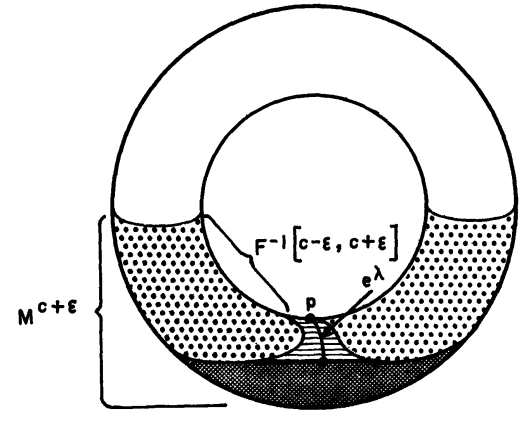
\includegraphics[width=0.5\textwidth]{32.png}
        \caption{32.png}
        \label{fig:32-png}
    \end{figure}

    \begin{proof}
        The idea of the proof of this theorem
        is indicated in \ref{fig:32-png} in
        the case of the height function on a torus.\\
        Here is the idea: we will introduce
        a new function $F \colon M \to \mathbb{R}$ 
        which coincides with the height function $f$ except
        that $F < f$ in a small neighborhood of the critical
        point $p$. Thus the region
        $F^{-1}(-\infty, c-\varepsilon]$ will consist
        of $M^{c-\varepsilon}$ together with a region
        $H$ near $p$ which we will call a "handle". More
        on that later.
        We will choose a suitable cell
        $e^{\lambda} \subset H$ and then
        pushing $H$ down onto $e^{\lambda}$ will give
        a deformation retract
        from $M^{c-\varepsilon} \cup  H$ to 
        $M^{c- \varepsilon} \cup  e^{\lambda}$.
        Then we will apply Theorem \ref{Thm:203191}
        to $F$ and the region
        $F^{-1}\left[ c-\varepsilon, c +\varepsilon \right] $
        giving a deformation retract of
        $M^{c-\varepsilon} \cup  H$ to $M^{c+\varepsilon}$.\\
        \linebreak
        Now, to the proof:\\
        Choose a coordinate system 
        $\left( u^{1},\ldots, u^{n} \right) $ 
        centered at $p$ so that
        \[
        f = c- \left( u^{1} \right)^2 - \ldots
        - \left( u^{\lambda} \right)^2 +
        \left( u^{\lambda+1} \right)^2 +\ldots +
        \left( u^{n} \right)^2
        \] 
        holds in $U$. \\
        Next, choose $\varepsilon > 0$ such that
        \begin{enumerate}
            \item $f^{-1}\left[ c-\varepsilon,
                c + \varepsilon\right] $ is compact
                and contains no critical points other
                than $p$.
            \item The image of $U$ under the diffeomorphism
                \[
                    \left( u^{1},\ldots,
                    u^{n}\right) \colon U \to 
                    \mathbb{R}^{n}
                \] 
                contains the closed ball
                \[
                \left\{ \left( u^{1},\ldots,
                u^{n}\right)  \mid 
            \sum \left( u^{i} \right)^2 \le 2\varepsilon 
        \right\} .
                \] 
        \end{enumerate}
        Now, we finally define 
        \[
        e^{\lambda} =
        \left\{ \left( u^{1},\ldots,
        u^{n}\right) \in U \mid 
    \sum_{i=1}^{\lambda} \left( u^{i} \right)^2 \le \varepsilon
    \quad \text{and} \quad
u^{\lambda+1} = \ldots = u^{n} = 0\right\} 
        \] 
        See Figure \ref{fig:3214255-png}.

        \begin{figure}[htpb]
            \centering
            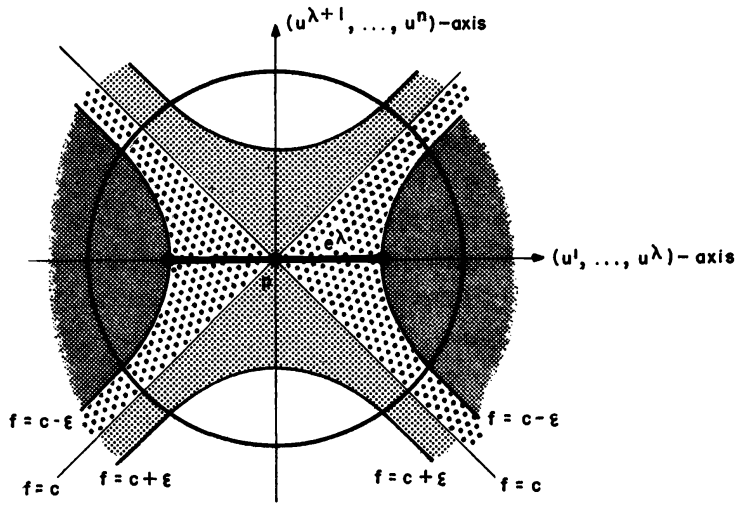
\includegraphics[width=0.8\textwidth]{3214255.png}
            \caption{Setup}
            \label{fig:3214255-png}
        \end{figure}
        The coordinate lines represent the planes
        $u^{\lambda+1} = \ldots = u^{n} = 0$ and
        $u^{1} = \ldots = u^{\lambda} = 0$, respectively.
        The circle represents the boundary of the ball of
        radius $\sqrt{2 \varepsilon} $, the
        hyperbolas represent the hypersurfaces
        $f^{-1}\left( c - \varepsilon \right) $ and
        $f^{-1}\left( c+\varepsilon \right) $. The
        region $M^{c-\varepsilon}$ is heavily shaded,
        the region $f^{-1}\left[ c-\varepsilon, c \right] $ 
        has big dots which are not so densely packed, while
        the region $f^{-1}\left[ c , c +\varepsilon \right] $ 
        has small dots which are tightly packed.
        The horizontal dark line through $p$ represents
        the cell $e^{\lambda}$.\\
        Note that $e^{\lambda} \cap
        M^{c- \varepsilon}$ is precisely the boundary
        $\partial e^{\lambda}$, so
        that $e^{\lambda}$ is attached to
        $M^{c -\varepsilon}$ as required.\\
        \linebreak

        Now we will construct a new function
        $F \colon M \to \mathbb{R}$. Let
        $\mu \colon \mathbb{R} \to \mathbb{R}$ e
        a smooth function such that
        $\mu (0) > \varepsilon,
        \mu (r) = 0$ for $r \ge 2 \varepsilon$ and
        $-1 < \mu'(r) \le 0$ for all $r$.
        Now let $F \equiv f$ outside of $U$ and
        on $U$,
        \[
        F = f - \mu \left( \sum_{i=1}^{\lambda}
        \left( u^{i} \right)^2 +
    2 \sum_{i=\lambda+1}^{n} \left( u^{i} \right)^2\right).
        \] 
        $F$ is clearly smooth.\\
        For convenience, let
        \[
        \xi, \eta \colon U \to [0,\infty)
        \] 
        be given by
        \begin{align*}
            \xi &= \sum_{i=1}^{\lambda}\left( u^{i} \right)^2\\
            \eta &= \sum_{i=\lambda+1}^{n} \left( u^{i} \right)^2
        \end{align*}

    so that
    $f = c - \xi + \eta$ and
    \[
    F(q) = c - \xi (q) + \eta(q) -
    \mu \left( \xi(q) + 2 \eta(q) \right) 
    \] 
    for all $q \in U$.
    
    \begin{assertion}
        The region $F^{-1}(-\infty, c+\varepsilon]$ coincides
        with the region $M^{c+\varepsilon} = 
        f^{-1}(-\infty, c+\varepsilon]$.
    \end{assertion}

    \begin{proof}
        Smth smth smth

    \underline{Verify the continuity in Case 2 later}

    \end{proof}

    \end{proof}

    \begin{remark}[]
        A modification of the proof of
        Theorem \ref{Thm:3890009} shows that
        the set $M^{c}$ is also a deformation retract
        of $M^{c+\varepsilon}$. In fact,
        $M^{c}$ is a deformation retract of
        $F^{-1}(-\infty, c]$ which is a deformation
        retract of $M^{c+\varepsilon}$.
        Combining this with Theorem \ref{Thm:3890009},
        we see that
        $M^{c- \varepsilon} \cup  e^{\lambda}$ 
        is a deformation retract of
        $M^{c}$.
    \end{remark}

    \begin{theorem}[]
        If $f$ is a smooth function on a manifold
        $M$ with no degenerate critical points, and
        if each $M^{a}$ is compact, then
        $M$ has the homotopy type of a CW-complex,
        with one cell of dimension $\lambda$ for each
        critical point of index $\lambda$.
    \end{theorem}

\newpage

    \begin{problem}[Reeb's Theorem]
        Let $M$ be a smooth, compact manifold
        of dimension $d$. Show that if $M$ admits
        a Morse function with only two critical points, then
        $M$ is homeomorphic to the sphere $S^{d}$. Indicate
        why the above proof fails in showing that $M$ is
        diffeomorphic to the sphere $S^{d}$.
    \end{problem}

    

    \subsection{The Cobordism Category}

    \begin{definition}[Smooth manifold triad]
        $\left( W; V_0,V_1 \right) $ is a smooth
        manifold triad if $W$ is a compact
        smooth $n$-manifold and $\partial W$ is the disjoint
        union of two open and closed submanifolds
        $V_0$ and $V_1$.
    \end{definition}

    \begin{definition}[]
        If $\left( W; V_0,V_1 \right) $ and
        $\left( W'; V_1', V_2' \right) $ are two
        smooth manifold triads and
        $h \colon V_1 \to V_1'$ is a diffeomorphism,
        then we can form a third triad
        $\left( W \cup_h W'; V_0, V_2' \right) $ where
        $W \cup_h W'$ is the space formed from
        $W$ and $W'$ by identifying points of
        $V_1$ and $V_1'$ under $h$ according to the
        following theorem.
    \end{definition}

    \begin{theorem}[]\label{sm-structure-cobordism-composition}
        There exists a smooth structure which is unique
        up to diffeomorphism fixing $V_0, h(V_1) = V_1'$ and
        $V_2'$ on
        $W \cup_h W'$  such that
        the inclusion maps
        $W \hookrightarrow W \cup_h W',
        W' \hookrightarrow W\cup_h W'$ are diffeomorphisms
        onto their images.
    \end{theorem}

    \begin{definition}[Cobordism]
        Given two closed smooth $n$-manifolds
        $M_0$ and $M_1$ (so $M_0,M_1$ compact and
        $\partial M_0 = \partial M_1 = \varnothing$ ),
        a \textit{cobordism} from
        $M_0$ to $M_1$ is a $5$-tuple
        $\left( W; V_0, V_1; h_0 , h_1 \right) $ where
        $\left( W; V_0, V_1 \right) $ is a smooth
        manifold triad and 
        $h_i \colon V_i \to M_i$ is a diffeomorphism for
        $i = 0,1$.
    \end{definition}


    \begin{definition}[Equivalence]
        Two cobordisms
        $\left( W;V_0,V_1;h_0,h_1 \right) $ and
        $\left( W';V_0',V_1';h_0',h_1' \right) $ from
        $M_0$ to $M_1$ are said to be \textit{equivalent} if
        there exists a diffeomorphism
        $g \colon W \to W'$ carrying $V_0$ to $V_0'$ 
        and $V_1$ to $V_1'$, such that for
        $i = 0,1$, the following triangle commutes:
        \begin{equation*}
        \begin{tikzcd}
            V_i \ar[rr, "g|_{V_i}"]\ar[dr, "h_i"']
            && V_i' \ar[dl, "h_i'"]\\
                                    & M_i &
        \end{tikzcd}
        \end{equation*}
    \end{definition}


    \begin{definition}[Composition of cobordisms]
        Given a cobordism equivalence class $c$ from
        $M_0$ to $M_1$ and $c'$ from
        $M_1$ to $M_2$, there
        is a well-defined class
        $ c c'$ from $M_0$ to $M_2$ formed
        using Theorem \ref{sm-structure-cobordism-composition} as
        follows:
        let 
        $\left( W; V_0, V_1; h_0, h_1 \right) $ be
        the cobordism from $M_0$ to $M_1$ and
        $\left( W'; V_0', V_1'; h_0',h_1' \right) $ 
        from $M_1$ to $M_2$.
        Then the cobordism formed by
        $\left( W \cup_{\id} W';
        V_0, V_1'; h_0, h_1'\right) $ 
        is a cobordism from $M_0$ to $M_2$, and
        furthermore, the inclusions
        $j_h \colon W \to W \cup_{\id} W'$ and
        $j_{h'} \colon W' \to 
        W \cup_{\id}W'$ are diffeomorphisms onto
        their images.\\

        This composition is
        associative.
    \end{definition}

    \begin{definition}[Identity cobordism]
        For every closed manifold $M$, the
        identity cobordism class
        $\iota_M $ is the equivalence class of
        $\left( M \times I; M \times 0,
        M \times 1 ; p_0 , p_1\right) $ where
        $p_i (x,i) = x$, for $x \in M$ and $i = 0,1$.
        Hence
        $\iota_{M_1} c = c  = c \iota_{M_2}$ when
        $c$ is a cobordism class from $M_1$ to $M_2$.
    \end{definition}

    \begin{definition}[Trivial cobordism]
        A cobordism $c = \left( W ; V_0, V_1; h_0,h_1 \right) $ 
        is called a trivial cobordism if it is
        equivalent to an identity cobordism.
    \end{definition}

    \begin{note}
        Note also that there
        are non-trivial inverses:
        \begin{figure}[htpb]
            \centering
            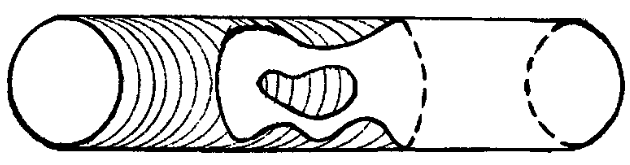
\includegraphics[width=0.8\textwidth]{cobordism-example-1.png}
            \label{fig:cobordism-example-1-png}
        \end{figure}
        In particular, the manifolds in a cobordism
        are \textbf{not} assumed to be connected.
    \end{note}

    \begin{definition}[]
        Consider cobordism classes from $M$ to itself.
        These form a monoid $H_M$. The invertible
        coboridisms in $H_M$ form a group $G_M$.
    \end{definition}

    \begin{definition}[$c_h$]
        Given a diffeomorphism
        $h \colon M \to M'$, define
        $c_h$ as the class of
        $\left( M \times I; M \times 0, M \times 1;
        j, h_1 \right) $ where
        $j (x,0) = x$ and
        $h_1 (x,1) = h(x)$ for $x \in M$.
    \end{definition}
    So a diffeomorphism
    $M \to M'$ gives a cobordism $c_h$ from $M$ to $M'$.

    \begin{theorem}[]
        $c_h c_h' = c_{h'h }$ for any two diffeomorphisms
        $h \colon M \to M'$ and
        $h' \colon M' \to M''$.
    \end{theorem}

    \begin{proof}
        Let
        $W = M \times I \cup_h M' \times I$.
        Let $c_h = \left( M \times I, M \times 0,
        M \times I, ; j_0, j_1 \right) $ and
        $c_{h'} = \left( 
        M' \times I, M' \times 0, M' \times 1,
    j_0', j_1' \right) $.
        So recall that this is formed by taking a tube
        on $M$ and a tube on $M'$ and then gluing an end
        of the tube of $M$ to an end of the tube of $M'$ through
        a twist by the diffeomorphism $h$. Then
        $W$ is still a smooth manifold.
        The resulting cobordism is
        $\left( W, M \times 0, M' \times 1,
        j_0, j_1' \right) $.
        We must show that this is the same, or more
        precisely, that this cobordism is
        \textit{equivalent} to the
        cobordism
        $\left( M \times I,
        M \times 0, M\times 1, j, h_1\right) $ where
        $j(x,0) = x$ and
        $h_1(x,1) = h'h (x)$.
        So we must define a
        diffeomorphism
        $g \colon M \times I \to W$ carrying
        $M \times 0$ to $M \times 0$ and
        $M \times 1$ to $M' \times I$, such that
        for $i = 0,1$, the following triangle commutes
        \begin{equation*}
        \begin{tikzcd}
            M \times 1 \ar[rr, "g|_{M \times 1}"] \ar[dr, "h_1"']
            && M' \times 1 \ar[dl, "j_1'"] \\
                               & M'' &
        \end{tikzcd}
        \end{equation*}
        and
        \begin{equation*}
        \begin{tikzcd}
            M \times 0 \ar[rr, "g|_{M \times 0}"] 
            \ar[dr, "j"] && M \times 0 \ar[dl, "j_0"]\\
                                       & M &
        \end{tikzcd}
        \end{equation*}

        Define
        $g \colon M \times I \to W$ by
        \[
        g(x,t) =
        \begin{cases}
            j_h(x,2t),& t \in \left[ 0 , \frac{1}{2} \right] \\
            j_{h'}\left( h(x), 2t-1 \right) ,& t\in 
            \left[ \frac{1}{2},1 \right] 
        \end{cases}
        \] 
        where
        $j_{h} \colon
        M \times I \to W$ is the inclusion and
        $j_{h'} \colon M' \times I \to W$ is
        the other inclusion given in the
        construction of
        $c_h c_{h'}$.
        Then indeed
        $g|_{M \times 0}$ maps
        into $M \times 0$ and
        $g|_{M \times 1}$ maps into
        $M' \times 1$.
        Furthermore,
        $j_0 \circ g(x,0) = 
        j_0 \circ j_h \left( x,0 \right) 
        = x$ and
        $j_1' \circ g(x,1) = 
        j_1' \circ j_{h'}\left( h(x),1 \right) 
        =j_1'  \left( h(x),1 \right) 
        = h'h(x)
        = h_1(x,1)$, so
        $j_1' \circ g = h_1$.
    \end{proof}

    \subsubsection{Isotopies and Pseudo-Isotopies}

    \begin{definition}[]
        Two diffeomorphisms
        $h_0,h_1 \colon M \to M'$ are
        (smoothly) isotopic if there exists a smooth map
        $f \colon M \times I \to M'$
        such that
        $f_t = f(-,t) \colon M \to M'$ is a diffeomorphism
        for every $t$ and
        $f_0 = h_0$ and $f_1 = h_1$.\\
        Two diffeomorphisms
        $h_0,h_1 \colon M \to M'$ are
        \textit{pseudo-isotopic} if there exists
        a diffeomorphism
        $g \colon M \times I \to M' \times I$ such that
        $g(x,0) = \left( h_0(x), 0 \right) $ and
        $g(x,1) = \left( h_1(x),1 \right) $.
    \end{definition}
    \begin{lemma}[]
        Isotopy and pseudo-isotopiy are equivalence
        relations.
    \end{lemma}

    \begin{theorem}[]
        $c_{h_0} = c_{h_1}$ if and only if
        $h_0$ is pseudo-isotopic to $h_1$.
    \end{theorem}

    \begin{proof}
        Let $g \colon M \times I \to M' \times I$ be a
        pseudo-isotopy between $h_0$ and $h_1$.
        Define
        $h_0^{-1} \times \id \colon M' \times I
        \to M \times I$ by
        \[
            \left( h_0^{-1} \times \id \right) (x,t)
            = \left( h_0^{-1}(x),t \right) .
        \] 
        We claim that
        $\left( h_0^{-1} \times \id \right) \circ g$ 
        is an equivalence 
        between $c_{h_1}$ and $c_{h_0}$.
        Firstly, 
        $\left( h_0^{-1}\times \id \right) 
        \circ g$ is indeed a map
        $M \times I \to M \times I$.
        If we write
        $c_{h_0} = 
        \left( M \times I; M \times 0,
        M \times 1; j_0, k_0 \right) $ and
        $c_{h_1} = \left( M \times I; M \times 0,
        M \times 1; j_0', k_0' \right) $ where
        $j_0(x,0) = x$,
        $j_0'(x,0) = x$ and
        $k_0(x,1) = h_0(x)$ and
        $k_0'(x,1) = h_1(x)$, then firstly,
        $\left( h_0^{-1}\times \id \right) \circ g
        (x,0) = \left( h_0^{-1} \times \id \right) 
        \left( h_0(x),0 \right) 
        = (x,0)$ and
        $\left( h_0^{-1} \times \id \right) \circ
        g(x,1) = \left( h_0^{-1} \times \id \right) 
        \left( h_1(x),1 \right) 
        = \left( h_0^{-1}\circ h_1(x),1 \right)
        \in M \times 1$, and lastly,

        \[
        k_0 \circ \left( h_0^{-1} \times \id \right) \circ g
        (x,1) = 
        k_0 \left( h_0^{-1} \circ h_1(x),1 \right) 
        = h_1(x) = 
        k_0' (x,1) 
        \] 
        and
        \[
        j_0 \circ \left( h_0^{-1} \times \id \right) 
        \circ g(x,0) = 
        j_0 (x,0) = x = 
        j_0' (x,0)
        \] 
        so
        $\left( h_0^{-1} \times \id \right) \circ g$ defines
        an equivalence from
        $c_{h_1}$ to $c_{h_0}$.
    \end{proof}


    \subsubsection{Interlude}

        A different way to define a cobordism is as follows:

        \begin{definition}[]
        A smooth compact $n$-dimensional manifold is
        said to be a cobordism between two $(n-1)$-dimensional
        smooth manifolds $M_L$ and $M_R$ if
        there exist open embeddings
        $M_L \times \mathbb{R} \hookrightarrow M$ and
        $M_R \times \mathbb{R} \hookrightarrow
        M$ such that
        the images of
        $M_R \times [0, \infty)$ and
        $M_L \times (-\infty, 0]$ are closed.
        We denote this by
        $M_L \rightsquigarrow M_R$
        \end{definition}

        \begin{definition}[Gluing cobordisms/composition
            of cobordisms]
            Given cobordisms $M_L \rightsquigarrow M_R =
            N_L \rightsquigarrow N_R$, we can
            form the composite cobordism
             $M \circ N$ as the pullback
             \begin{equation*}
             \begin{tikzcd}
                 M_L \times \mathbb{R}
                 \ar[dr, hookrightarrow]&& M_R \times \mathbb{R}
                 = N_L \times R \ar[dl, hookrightarrow] \ar[dr,
                 hookrightarrow]
                                       && N_R \times \mathbb{R} 
                                       \ar[dl, hookrightarrow]\\
                                       &M \ar[dr, hookrightarrow]&&
                 N\ar[dl, hookrightarrow]&\\
                 &&M \circ N \ar[uu, phantom, "\lrcorner" labl, very
                 near start]&&
             \end{tikzcd}
             \end{equation*}
        \end{definition}


        \begin{definition}[Isomorphism/Equivalence of Cobordisms]
            In this definition, two
            cobordisms
            $M_1 \colon M_L \rightsquigarrow M_R$ and
            $M_2 \colon M_L \rightsquigarrow M_R$ are
            isomorphic/equivalent when there exist maps
            making the following diagram commute:
            \begin{equation*}
            \begin{tikzcd}
                M_L \times R \ar[r, hookrightarrow]
                \ar[d, dash, "\id"']
                & M_1 \ar[d, "f"', "\cong"] & M_R
                \times \mathbb{R} \ar[l, hookrightarrow]
                \ar[d, dash, "\id"] \\
                M_L \times \mathbb{R} \ar[r, hookrightarrow]
                & M_2 & M_R \times 
                \mathbb{R} \ar[l, hookrightarrow]
            \end{tikzcd}
            \end{equation*}
        \end{definition}


        \begin{definition}[Identity cobordism]
            For a smooth compact manifold $M$, the
            identity cobordism of $M$ is the cobordism
            from  $M$ to $M$ given by
            $M \times \mathbb{R}$ where
            we embed
            $M \times \mathbb{R}_{<0} \hookrightarrow
            M \times \mathbb{R}$ 
            and $M \times \mathbb{R}_{>0} 
            \hookrightarrow M \times \mathbb{R}$ by
            the inclusions.
        \end{definition}

        \begin{definition}[Trivial cobordism]
            A cobordism is trivial if it is equivalent to
            an identity cobordism.
        \end{definition}


        \subsection{Elementary Cobordisms}

        \begin{definition}[Gradient-like vector fields for
            Morse functions]
            Let $f$ be a Morse function for the
            triad 
            $\left( W^{n}; V, V' \right) $. A vector field
            $\xi$ on $W^{n}$ is a \textit{gradient-like
            vector field for $f$} if
            \begin{enumerate}
                \item $\xi (f) >0$ throughout the complement
                    of the set of critical points of $f$
                \item Given any critical point $p$ of $f$,
                    there are coordinates
                    $\left( x,y \right) =
                    \left( x_1, \ldots, x_{\lambda},
                    x_{\lambda +1}, \ldots,
                x_n\right) $ in a neighborhood $U$ of $p$ 
                such that
                $f = f(p) - \left| x \right|^2 +
                \left| y \right|^2$ and
                $\xi$ has coordinates
                $\left( -x_1, \ldots, -x_{\lambda},
                x_{\lambda +1}, \ldots,
            x_n\right) $ throughout $U$.
            \end{enumerate}
        \end{definition}

        \begin{remark}[]
            The first condition essentially says
            that outside the critical points of
            $f$, $\xi$ points in the direction into
            which $f$ is increasing. If
            we think of $f$ as a height function for
            the manifold, then $\xi$ points "upward" along
            the manifold. 
        \end{remark}

        \begin{figure}[htpb]
            \centering
            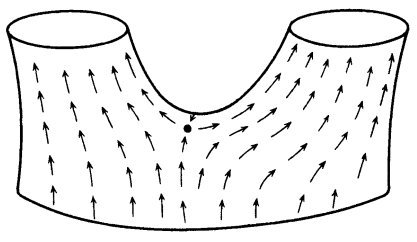
\includegraphics[width=0.4\textwidth]{gradient-like-vector-field.png}
            \caption{A gradient-like vector field}
            \label{fig:gradient-like-vector-field-png}
        \end{figure}

        \begin{theorem}[]
            Let $f \colon M \to \mathbb{R}$ be a Morse
            function on a compact manifold $M$. Then
            there exists a gradient-like vector field
            $\xi$ for $f$.
        \end{theorem}

        \begin{definition}[]
            If $\xi$ is a vector field on $M$, an
            \textit{integral curve of $\xi$} is a smooth
            curve $\gamma \colon J \to M$ 
            such that
            \[
            \gamma'(t) = \xi_{\gamma(t)}, \forall t \in J
            \] 
        \end{definition}

        \begin{proposition}[]
            \cite[Prop 9.2]{LeeSM}
            Let $\xi$ be a smooth vector field on a smooth
            manifold $M$. For each point $p \in M$, there
            exists $\varepsilon > 0$ and a smooth curve
            $\gamma \colon (-\varepsilon, \varepsilon) \to M$ that
            is an integral curve of $V$ starting at $p$.
        \end{proposition}



        \begin{remark}[]
            We identify the triad
            $\left( W; V_0, V_1 \right) $ with the
            cobordism
            $\left( W; V_0, V_1 ; i_0, i_1 \right) $ where
            $i_0 \colon V_0 \to V_0 $ and
            $i_1 \colon V_1 \to V_1$ are the identity maps.
        \end{remark}

        \begin{definition}[Product cobordism]
            A triad $\left( W; V_0,V_1 \right)  $ is said
            to be a \textit{product cobordism} if it
            is diffeomorphic to the trivial cobordism
            $\left( V_0 \times \left[ 0,1 \right] ; V_0
            \times 0, V_0 \times 1\right) $.
        \end{definition}

        \begin{theorem}[Identifying product/trivial cobordisms]
            If the Morse number $\mu$ of a triad
            $\left( W; V_0, V_1 \right) $ is zero, then
            $\left( W; V_0,V_1 \right) $ is a product cobordism.
        \end{theorem}

        \begin{proof}
            Let $f \colon W \to \mathbb{R}$ be a Morse function
            with no critical points. 
            Since $W$ is compact, we have
            $f(W) = \left[ a,b \right] $.
            Choose a gradient-like vector field
            $\xi$ for $f$. As $\xi (f) > 0$ on all
            of $W$, we can define a new
            vector field $\zeta$ on $W$ by
            \[
            \zeta = \frac{1}{\xi (f)} \xi.
            \] 
            Consider the integral curve
            $c_p(t)$ of $\zeta$ starting at a 
            point $p$ of $f^{-1}(a)$. Then
            \begin{align*}
                \frac{d}{dt} f\left( c_p(t) \right) 
                = c'(t) f
                = \zeta_{c(t)} (f)
                = \frac{1}{\xi (f)} \xi (f)
                = 1
            \end{align*}
        Since it starts at the level set
        $f = a$ at time $t = 0$, it will reach the
        level set $f = b$ at time
        $t = b-a$. Define a map
        $h \colon f^{-1}(a) \times \left[ 0, b-a \right] 
        \to W = W_{[a,b]}$ by
        \[
        h(p,t) = c_{p(t)}.
        \] 
        The proof follows from $h$ being a diffeomorphism
        as it depends smoothly on $p $ and $t$ and that
    two distinct integral curves do not meet.
        \end{proof}

        \begin{theorem}[Collar Neighborhood Theorem]
            Let $W$ be a compact smooth manifold with
            boundary. There exists a neighborhood of
            $\partial W$ (called a collar neighborhood)
            diffeomorphic to 
            $\partial W \times [0,1)$.
        \end{theorem}

        \begin{definition}[Two-sided]
            A connected, closed submanifold
            $M^{n-1} \subset 
            W^{n} - \partial W^{n}$ is said to be
            \textit{two-sided} if some neighborhood
            of $M^{n-1}$ on $W^{n}$ is cut
            into two components when $M^{n-1}$ is deleted.
        \end{definition}


        \begin{theorem}[The Bicollaring Theorem]
            Suppose that every component of
            a smooth submanifold $M$ of $W$ is
            compact and two-sided. Then there
            exists a "bicollar" neighborhood of
            $M$ in $W$ diffeomorphic to
            $M \times (-1,1)$ in such a way that
            $M$ corresponds to
            $M \times 0$.
        \end{theorem}


\subsubsection{Handlebody decomposition/surgery}


First, the setup.\\
Suppose $\left( W; V,V' \right) $ is a triad with
Morse function $f \colon W \to \mathbb{R}$ and
gradient-like vector field $\xi$ for $f$.
Suppose $p \in W$ is a critical point, and
$V_0 = f^{-1}(c_0)$ and
$V_1 = f^{-1}(c_1)$ are level sets such that
$c_0 < f(p) < c_1$ and that
$c = f(p)$ is the only critical value in the interval
$\left[ c_0,c_1 \right] $.

Now, since $\xi$ is a gradient-like vector field for
$f$, there exists a neighborhood $U$ of $p$ in $W$
and a coordinate diffeomorphism
$ g \colon B(0, 2 \varepsilon) \to U$ such that
$f \circ g  (x,y) = 
c - \|x\|^2 + \|y\|^2 $ and
so that $\xi$ has coordinates
$\left( -x_1, \ldots, -x_{\lambda},
x_{\lambda+1}, \ldots, x_n\right) $ throughout $U$, for
some $-1 \le \lambda \le n$ and some
$\varepsilon > 0$.\\
Now let $V_{-\varepsilon} =
f^{-1}\left( c- \varepsilon^2 \right) $ and
$V_{\varepsilon} = f^{-1}\left( c+ \varepsilon^2 \right) $.
We may assume that
$4 \varepsilon^2 < \min \left\{ \left| c-c_0 \right| ,
\left| c-c_1 \right| \right\} $ so that
$V_{-\varepsilon}$ lies between
$V_0$ and $f^{-1}(c)$ and
$V_{\varepsilon}$ lies between $f^{-1}(c) $ and
$V_1$.

\begin{definition}[Characteristic embedding]
    The characteristic embedding
    $\varphi_{L} \colon S^{\lambda-1} \times 
    B^{n - \lambda} \to V_0$ is obtained as follows.\\
    First, define an embedding
    $\varphi \colon S^{\lambda-1} \times 
    B^{n-\lambda} \to V_{-\varepsilon}$ by
    $\varphi \left( u, \theta v \right) =
    g \left( \varepsilon u \cosh \theta,
    \varepsilon v \sinh \theta \right) $ for
    $u \in S^{\lambda-1}, v \in S^{n-\lambda-1}$ and
    $0 \le \theta < 1$.
    Then
    $f \circ \varphi \left( u , \theta v \right) 
    = c - \|\varepsilon u \cosh \theta\|^2
    + \| \varepsilon v \sinh \theta \|^2
    = c - \varepsilon^2 $, so indeed,
    $\varphi \left( u, \theta v \right) \in 
    V_{-\varepsilon}$.
    Since $\varphi $ is also an injective
    continuous map from a compact space to a Hausdorff space,
    it is an embedding.\\
    Starting now at the point
    $\varphi \left( u, \theta v \right) \in V_{- \varepsilon}$,
    the integral curve of $\xi$ (which, recall, goes
    "upward") is a non-singular (non-vanishing
    Jacobian) curve which leads
    from $\varphi \left( u, \theta v \right) $ back to
    some well-defined point $\varphi_L \left( u,
    \theta v\right)  \in V_0$.\\
    Define the \textit{left-hand sphere} $S_L$ of
    $p$ in $V_0$ to be the image
    $\varphi_L \left( S^{\lambda-1} \times 0 \right) $.
\end{definition}


\begin{figure}[htpb]
    \centering
    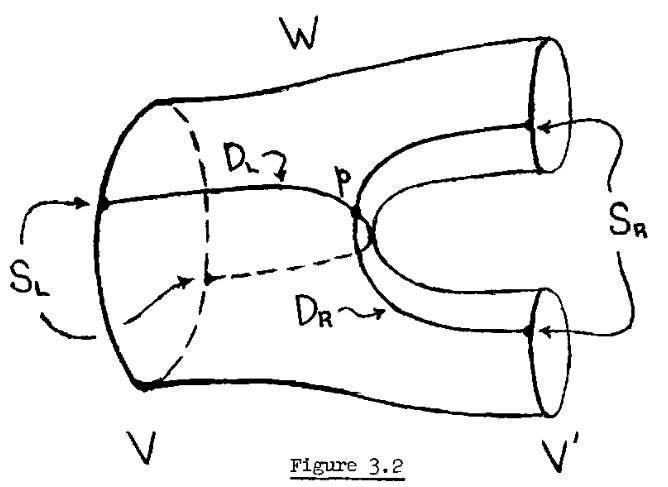
\includegraphics[width=0.7\textwidth]{fig3-2.png}
    \label{fig:fig3-2-png}
\end{figure}



\begin{definition}[Surgery]
    Given a manifold $V$ of dimension $n-1$ and
    an embedding $\varphi  \colon S^{\lambda - 1}\times 
    B^{n-\lambda} \to V$, let
    $\chi (V, \varphi )$ denote the quotient manifold obtained
    from the disjoint union
    \[
        \left( V - \varphi \left( S^{\lambda-1}\times 0 \right) 
        \right) \sqcup \left( B^{\lambda} \times 
        S^{n-\lambda-1} \right) 
    \] 
    by identifying $\varphi (u, \theta v)$ with
    $\left( \theta u, v \right) $ for
    each $u \in S^{\lambda-1}, v \in S^{n-\lambda-1}$ and
    $0 < \theta < 1$. If
    $V'$ denotes any manifold diffeomorphic to
    $\chi (V, \varphi )$ then we will say that
    $V'$ can be obtained from $V$ by \textit{surgery} of
    type $\left( \lambda, n-\lambda \right) $.
\end{definition}


So surgery on an $(n-1)$-manifold has the effect
of removing an embedded sphere of dimension $\lambda-1$ 
and replacing it by an embedded sphere of dimension
$n - \lambda - 1$.

   \begin{definition}[]
       An \textit{elementary cobordism} is a triad
       $\left( W; V, V' \right) $ possessing a Morse
       function $f$ with exactly one critical point
       $p$.
   \end{definition}


\begin{theorem}[]
    If $V' = \chi (V, \varphi )$ can be obtained from
    $V$ by surgery of type $\left( \lambda, n-\lambda
    \right) $, then there exists an elementary cobordism
    $\left( W; V,V' \right) $ and a Morse function
    $f \colon M \to \mathbb{R}$ with
    exactly one critical point of index $\lambda$.
\end{theorem}

\begin{proof}
    Let
    \[
    L_{\lambda} = 
    \left\{ \left( x,y \right) 
    \in \mathbb{R}^{\lambda} \times 
\mathbb{R}^{n-\lambda}  \mid 
-1 \le - \|x\|^2 + \|y\|^2 \le 1,
\|x\|\|y\| < \sinh 1 \cosh 1\right\},
    \] 
    which is a manifold with two boundaries:
    the "left" boundary
    $\left\{ -\|x\|^2+ \|y\|^2 = -1 \right\} $ is
    diffeomorphic to
    $S^{\lambda-1} \times B^{n-\lambda}$.
    Indeed, recall that
    \[
    \cosh^2 x - \sinh^2 x = 1,
    \] 
    and consider the
    map
    \[
        \left( u, \theta v \right) 
        \mapsto \left( u \cosh \theta, v
        \sinh \theta \right) 
    \] 
    Show that it is a diffeomorphism. Similarly for
    the "right" boundary.

    \begin{figure}[htpb]
        \centering
        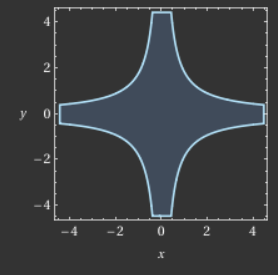
\includegraphics[width=0.3\textwidth]{xy-graph.png}
        \caption{$\left| xy \right| < \sinh 1 \cosh 1$}
        \label{fig:xy-graph-png}
    \end{figure}

    \begin{figure}[htpb]
        \centering
        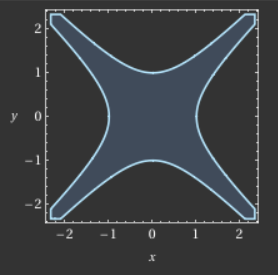
\includegraphics[width=0.3\textwidth]{y^2-x^2-graph.png}
        \caption{$-1 \le -\|x\|^2 + \|y\|^2 \le 1$}
        \label{fig:y-2-x-2-graph-png}
    \end{figure}


    Consider the orthogonal trajectories of
    the surfaces $-\|x\|^2 + \|y\|^2 = \text{constant}$.

    The trajectories of the surface
    $- \|x\|^2 + \|y\|^2 = c$ can be parametrized
    by
    $t \mapsto \left( t x, t^{-1} y \right) $. 
    To see this, pick a point
    $(x,y) $ such that
    $-\|x\|^2 + \|y\|^2 = c$, that is

    $(x,y) = \left( c u \sinh \theta, c v \cosh \theta \right) $.
    Then the derivative with respect to $\theta$ is
    \[
        \left( c u \cosh \theta,
        c v \sinh \theta \right) 
    \] 
    and since
    \[
        \left( c u \cosh \theta,
        c v \sinh \theta\right) \cdot 
        \left( cu \sinh \theta, - cv \cosh \theta \right) 
        = c^2 \left( \|u\|^2 \cosh \theta \sinh \theta
        - \|v\|^2 \cosh \theta \sinh \theta \right) 
        = 0
    \] 
    since $\|u\|=\|v\| = 1$.


    \begin{figure}[htpb]
        \centering
        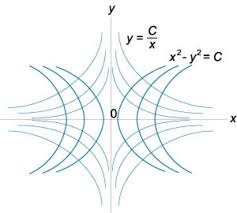
\includegraphics[width=0.5\textwidth]{level-sets.jpeg}
        \caption{level-sets.jpeg}
        \label{fig:level-sets-jpeg}
    \end{figure}

    We now construct a manifold
    $W = \omega \left( V, \varphi  \right) $ as follows.
    Start with the disjoint union
    \[
        \left( V - \varphi 
        \left( S^{\lambda-1} \times 0 \right) \right) \times 
        D^{1} \sqcup L_{\lambda}.
    \] 
    Now for each $u \in S^{\lambda-1}, v\in 
    S^{n-\lambda-1}, 0 < \theta < 1$ and
    $c \in D^{1}$, identify the point
    $\left( \varphi (u,\theta v), c \right) $ in the
    first summand with the point
    $\left( x,y  \right) \in L_{\lambda}$ such that
    \begin{enumerate}
        \item $- \|x\|^2 + \|y\|^2 = c$ 
        \item $\left( x,y \right) $ lies on the orthogonal
            trajectory which passes through the point
            $\left( u \cosh \theta, v \sinh \theta \right) $.
    \end{enumerate}
    This defines a diffeomorphism
    \[
    \varphi \left( S^{\lambda-1} \times 
    \left( B^{n-\lambda} - 0 \right) \right) \times D^{1}
    \cong L_{\lambda} \cap
    \left( \mathbb{R}^{\lambda}-0 \right) \times
    \left( \mathbb{R}^{n-\lambda}
    -0\right) 
    \] 

    (Finish the proof)

\end{proof}


\begin{theorem}[]
    Let $\left( W; V, V' \right) $ be an elementary cobordism
    with characteristic embedding
    $\varphi_L \colon S^{\lambda-1} \times 
    B^{n-\lambda} \to V$. Then
    $\left( W; V, V' \right) $ is diffeomorphic to
    the triad $\left( \omega (V, \varphi_L); V,
    \chi \left( V, \varphi_L \right) \right) $.
\end{theorem}

\begin{theorem}[]
    Let $\left( W; V,V' \right) $ be an elementary
    cobordism possessing a Morse function with one
    critical point, of index $\lambda$. Let
    $D_L$ be the left-hand disk associated to a fixed
    gradient-like vector field. Then
    $V \cup  D_L$ is a deformation retract of $W$.
\end{theorem}

\begin{corollary}
    \[
    H_n (W,V)
    \cong
    \begin{cases}
        \mathbb{Z},& n= \lambda\\
        0,& n\neq \lambda
    \end{cases}.
    \] 
    A generator for $H_{\lambda}(W,V)$ is represented
    by $D_L$.
\end{corollary}



        \newpage

        \subsubsection{Problems}

    \begin{problem}[Invertible cobordisms and boundaries of
        compact manifolds]
        Let 
        $W_0 \colon M_0 \rightsquigarrow \varnothing $ and
        $W_1 \colon M_1 \rightsquigarrow \varnothing$ be
        two compact $d$-dimensional smooth cobordisms
        from compact $\left( d-1 \right) $-dimensional
        smooth manifolds $M_0$ and $M_1$ to the
        empty manifold, viewed as a 
        $\left( d-1 \right) $-manifold. In other words,
        we have a smooth embedding
        $M_i \times \mathbb{R} \hookrightarrow W_i$ satisfying
        that $M_i \times (-\infty, 0]$ is
        closed, and such that
        their complement 
        $W_i - \left( M_i \times \mathbb{R} \right) $ 
        is compact. We define
        $\Int \left( W_i \right) $ to
        be the complement of the image of
        $M_i \times (- \infty, t]$ for some $t \in \mathbb{R}$ 
        (and hence any $t \in \mathbb{R}$), and observe
        that $\Int \left( W_i \right) $ is again a
        smooth manifold, being an open subset of $W_i$.
        \begin{enumerate}
            \item Assume that in the situation of the
                above, $\Int (W_0)$ is diffeomorphic
                to $\Int \left( W_1 \right) $. Show that
                $M_0$ and $M_1$ are invertibly cobordant,
                i.e., there exists a cobordism
                $M_0 \rightsquigarrow M_1$ which is invertible
                in the category $\Cob_d$.
            \item Let $W$ be a smooth, open
                (i.e., non-compact) $d$-manifold. We define
                a compact closure of $W$ to be a compact
                cobordism $W' \colon
                M \rightsquigarrow \varnothing$ such that
                $W$ is diffeomorphic to 
                $\Int (W')$. Assume that $W$ admits
                a comapct closure $W' \colon M \rightsquigarrow
                \varnothing$. Show that the set of
                compact closures of $W$ up to isomorphism
                of their interiors is in bijection with the
                set of invertible cobordisms over $M$.
        \end{enumerate}
    \end{problem}

    \begin{proof}
        (1)

         Saying that
        $M_0 \rightsquigarrow M_1$ is invertible
        in $\Cob_d$ is precisely saying that
        there exists a cobordism
        $M_1 \rightsquigarrow M_0$ such that the
        composite cobordism
        $M_0 \rightsquigarrow M_1\rightsquigarrow M_0$ 
        is equivalent to the trivial cobordism
        $M_0 \rightsquigarrow M_0$. We
        will do this using the usual definition
        of cobordisms with boundaries. Then
        the problem is equivalently to show that
        we can find coborisms
        $M_0 \rightsquigarrow M_1\rightsquigarrow M_0$ 
        such that
        the composite
        is a product cobordism - i.e., has Morse number
        $0$.
        In this case, we are dealing with closed
        compact manifolds
        $W_0, W_1$ such that
        $\partial W_0 \cong M_0$ and
        $\partial W_1 \cong M_1$. Furthermore,
        the boundaries have closed collar
        neighborhoods
        $\partial W_i \times I$, and removing some open/usual collar
        neighborhoods of these boundaries $\partial W_i \times 
        [0,1)$
        leaves us with compact spaces which are, by
        assumption, diffeomorphic.
        Now, take
        the cobordism $W_0$ and choose
        a collar neighborhood of $\partial W_0 $:
        $M_0 \times [0,1]$, where
        $M_0$ is identified with $M_0 \times 0$ in $W_0$.
        By assumption, there is a diffeomorphism
        $W_0 - \left( M_0 \times [0,1] \right) 
        \cong W_1 - \left( M_1 \times [0,1] \right) $.
        Now, the diffeomorphism
        extends to the closure of the interiors
        which is also $M_i$ since the collar is a cylinder, so
        we obtain a diffeomorphism
        $h \colon M_0 \times 1 \cong M_1 \times 1$. Without
        loss of generality, we can reparametrize, to get the
        diffeomorphism
        $h \colon M_0 \times 1 \to M_1 \times 0$ since
        the boundaries of the interiors must map to each other.
        Now we can glue the collars by gluing the cobordisms
        they represent using theorem 1.4 in Milnor's book
        on h-cobordisms to get a cobordism
        $c_h $ which is the manifold
        $M_0 \times [0,1] \cup_h M_1 \times [0,1]$.
        This indeed now gives a cobordism
        $M_0 \rightsquigarrow M_1$. We can likewise
        obtain the cobordism
        $M_1  \rightsquigarrow M_0 $ which is also obtained
        by gluing
        $M_1 \times [0,1]$ with $M_0\times  [0,1]$ along
        $M_1 \times 1$ and $M_0 \times 0$. Denote this
        cobordism by $c_{h'}$.
        We claim that $c_{h} c_{h'} = \id_{M_0}$. That is, that
        $c_{h} c_{h'}$ is a product cobordism/trivial cobordism
        of $M_0$. One way to see this is
        by using theorem 1.6 in Milnor's book on $h$-cobordisms
        which says that
        $c_{h} c_{h'} = c_{h' h} = c_{\id_{M_0}}$ which indeed
        is the trivial cobordism.
        Alternatively, each collar neighborhood has no
        critical values, so 
        $c_h$ and $c_{h'}$ both have Morse number $0$, and
        then corollary 3.8 in Milnor's book on
        $h$-cobordisms gives that
        $c_h c_{h'}$ also has Morse number $0$, hence
        is trivial by theorem 3.4 in the same book.
    \end{proof}



    \newpage


    \subsection{Morse Functions}

    The goal is to be able to factor cobordisms into
    compositions of simpler cobordisms.

    \begin{definition}[Critical points and non-degenerate
        critical points]
        Let $W$ be a smooth manifold and
        $f \colon W \to \mathbb{R}$ a smooth function.
        A point $p \in W$ is a critical point of
        $f$ if, in some coordinate system,
        \[
        \frac{\partial f}{\partial x^{1}}|_{p} = 
        \frac{\partial f}{\partial x^2}|_{p} = \ldots 
        = \frac{\partial f}{\partial x^{n}}|_p = 0.
        \] 
        Such a point is called a non-degenerate critical
        point if $\det \left( H(f)_p \right) 
        = \det \left( \frac{\partial^2 f}{\partial x^{i}
        \partial x^{j}}|_p \right) \neq 0$
    \end{definition}

    \begin{lemma}[Morse Lemma]\label{Morse-Lemma}
        If $p$ is a non-degenerate critical point of
        $f$, then in some coordiante system about $p$,
        \[
        f\left( x_1, \ldots, x_n \right) =
        c - x_1^2 - \ldots - x_{\lambda}^2 +
        x_{\lambda+1}^2 + \ldots + x_{n}^2
        \] 
        for $\lambda$ between $0$ and $n$ and
        $c$ some constant.
    \end{lemma}

   \begin{definition}[Index of a critical point]
       The $\lambda$ from the Morse Lemma (Lemma~\ref{Morse-Lemma})
       is called the index of the critical point $p$.
   \end{definition} 

   \begin{definition}[Morse Function]
       A \textit{Morse function} on a smooth
       manifold triad
       $\left( W; V_0,V_1 \right) $ is a smooth
       function $f \colon W \to \left[ a,b \right] $ 
       such that
       \begin{enumerate}
           \item $f^{-1}(a) = V_0$ and $f^{-1}(b) = V_1$ 
           \item All the critical points of $f$ are
               interior (lie in $W - \partial W$ ) and
               are non-degenerate.
       \end{enumerate}
   \end{definition}

   \begin{corollary}
       A Morse function has only finitely many zeros.
   \end{corollary}

   \begin{proof}
       Suppose we have a Morse function
       $f \colon W \to \left[ a,b \right] $ and
       suppose that  $p$ is
       a critical point. By definition, it is non-degenerate
       since $f$ is a Morse function, so by the
       Morse Lemma, in some neighborhood of
        $p$, $f$ takes the form
       \[
       f\left( x_1, \ldots, x_n \right) 
       = c - x_1^2 - \ldots - x_{\lambda}^2 +
       x_{\lambda+1}^2 + \ldots+ x_{n}^2
       \] 
       so in particular,
       $\frac{\partial f}{\partial x^{i}} 
       \left( x_1,\ldots,x_n \right) 
       = -2x_i$ in this neighborhood for all $i$.
       Hence $\left( x_1, \ldots, x_n \right) 
       = \left( 0,\ldots,0 \right) $ in this neighborhood
       is the only critical point (in particular,
       in local coordinates, $p = \left( 0,\ldots,0 \right) $ ).
       This shows that critical points of a Morse
       function are isolated. Since
       the manifold of a smooth manifold triad is, in particular,
       compact, there are only finitely many critical points
       since a collection of isolated points in a compact
       space is finite.
   \end{proof}

   \begin{definition}[Morse number $\mu$]
       The \textit{Morse number} $\mu$ of $\left( W;
       V_0, V_1\right) $ is the minimum over all
       Morse functions $f$ on $\left( W;V_0,V_1 \right)$
       of the number of critical
       points of $f$.
   \end{definition}

   \begin{theorem}[Existence of
       Morse functions]\label{Existence-of-Morse-functions}
       Every smooth manifold triad
       $\left( W;V_0,V_1 \right) $ possesses
       a Morse function.
   \end{theorem}

   \begin{remark}[]
       We proved a stronger version of this theorem
       in Problem \ref{Problem:Existence-Morse-Functions}.
       We will also outline the proof idea from Milnor's book.
   \end{remark}

   To prove the existence theorem of Morse functions, 
   we need the following lemmas:

   \begin{lemma}[]
       There exists a smooth function
       $f \colon W \to \left[ 0,1 \right] $ with
       $f^{-1}(0) = V_0, f^{-1}(1) = V_1$, such that
       $f$ has no critical points in a neighborhood
       of the boundary of $W$.
   \end{lemma}

   \begin{lemma}[M. Morse]
       If $f$ is a $C^2$ mapping of an open subset
       $U \subset R^{n}$ to the real line, then,
       for almost all linear mappings
       $L \colon R^{n} \to R$, the function
       $f + L$ has only nondegenerate critical
       points.
   \end{lemma}

   \begin{proof}
       The idea of the proof is
       to consider the manifold
       $U \times \Hom_{\mathbb{R}} \left( \mathbb{R}^{n},
       \mathbb{R} \right) $ the its submanifold
       $M = 
       \left\{ \left( x,L \right)  \mid 
       d\left( f(x) + L(x) \right) = 0\right\} $.
       Then $x\mapsto \left( x,-df(x) \right) $ is
       a diffeomorphism $U \cong M$. Composing with
       a projection $\pi \colon M \to \Hom\left( \mathbb{R}^{n},
       \mathbb{R}\right) $ sending
       $\left( x,L \right) \mapsto L$, which,
       under the identification, corresponds to
       $x \mapsto -df(x)$; one sees that
       $\pi$ is critical at $x \approx \left( x,L \right) \in M
       \cong U$ 
       if and only if
       $d\pi = - \frac{\partial^2 f}{\partial x_i 
       \partial x_j}$ is singular.
       So $x$ is a degenerate critical point of $f + L$ 
       if and only if it is a critical point of
       $\pi$. By Sard's theorem, the set of critical
       values of $\pi$ has measure zero. So
       if we can show that the
       image of $\pi$ does not have measure zero, the result follows.
       For this, notice that
       $\pi$ maps $x \mapsto -df(x)$ and we have
       a diffeomorphism
       $U \cong M$ by
       $x \mapsto \left( x, -df(x) \right) $, so
       $\pi$ is an open map from
       $U$ into $\mathbb{R}^{n}$, hence
       in particular, the image is open and thus
       not measure zero.
   \end{proof}

   \begin{lemma}[Lemma B]
       Let $K$ be a compact subset of an
       open set $U \subset \mathbb{R}^{n}$. If
       $f \colon U \to \mathbb{R}$ is  $C^2$ and
       has only nondegenerate critical points in
       $K$, then there is a number $\delta >0$ such that
       if $g \colon U \to \mathbb{R}$ is $C^2$ and at
       all points of $K$, we have
        \[
       \left| \frac{\partial f}{\partial x_i} -
       \frac{\partial g}{\partial x_i} \right| < \delta,
       \quad
       \left| \frac{\partial^2 f}{\partial x_i \partial x_j}
       - \frac{\partial^2 g}{\partial x_i \partial x_j}\right| <
       \delta 
       \] 
       for $i,j = 1,\ldots, n$, then
       $g$ likewise has only nondegenerate critical points
       in $K$.
   \end{lemma}

   \begin{proof}
       Just an extra note on the proof: 
       \[
       \left| \left| df \right| -
       \left| dg \right| \right|^2
       \le \left| df - dg \right|^2
       = \left| d(f-g) \right|^2
       = \sum_i \left|   \frac{\partial f}{\partial x_i}
       - \frac{\partial g}{\partial x_i}\right|^2
       \] 
       giving the possibility of bounding
       this by $\frac{\mu}{2}$.
       The other bound is done similarly.
   \end{proof}
        
   \begin{lemma}[Lemma C]
       Suppose $h \colon U \to U'$ is a diffeomorphism
       of one open subset of $\mathbb{R}^{n}$ onto
       another and carries the compact set
       $K \subset U$ onto $K' \subset U'$. Given
       a number $\varepsilon > 0$, there is a number
       $\delta > 0$ such that if a smooth map
       $f \colon U' \to \mathbb{R}$ satisfies
       \[
       \left| f \right| < \delta, \quad
       \left| \frac{\partial f}{\partial x_i} \right| <
       \delta,
       \quad
       \left| \frac{\partial^2 f}{\partial x_i \partial
       x_j} \right| < \delta,
       \quad i, j = 1,\ldots,n
       \] 
       at all points of $K' \subset U'$, then
       $f \circ h$ satisfies
       \[
       \left| f \circ h \right| <
       \varepsilon, \quad
       \left| \frac{\partial f \circ h}{\partial x_i} \right| 
       < \varepsilon,
       \quad
       \left| \frac{\partial^2 f \circ h}{\partial x_i
       \partial x_j} \right| < \varepsilon,
       \quad
       i , j = 1,\ldots, n
       \] 
       at all points of $K$.
   \end{lemma}

   \begin{definition}[The compact-open $C^2$ topology]
       \cite[p. 34]{Hirsch}
       What Milnor calls the $C^2$ topology
       on $F \left( M, \mathbb{R} \right) $ of smooth
       real-valued functions on a compact manifold,
       $M$ with boundary is, I believe,
       simply the compact-open $C^2$ topology on
       $F \left( M, \mathbb{R} \right)=
       C^{\infty}(M)$.

       The compact open topology on
       $F \left( M, \mathbb{R} \right) $ is generated
       by sets defined as follows. Let
       $f \in F \left( M, \mathbb{R} \right) $ and
       $\left( \varphi ,U \right) $ a chart on
       $M$. Let $K \subset U$ be compact. Define a weak
       subbasic neighborhood
       \[
       \mathcal{N}^2 \left( f; \left( \varphi ,U \right) ,
       K, \varepsilon\right) 
       \] 
       to be the set of all
       smooth maps $g \colon M \to \mathbb{R}$ such that
        \[
       \| D^{k}\left( f \varphi^{-1} \right) (x)
       - D^{k}\left( g \varphi^{-1} \right) (x)\|< \varepsilon
       \] 
       for all $x \in \varphi (K)$, $k = 0, 1,2$.
       The $C^2$ topology on
       $F \left( M, \mathbb{R} \right) $ is generated
       by these sets.
   \end{definition}


   \begin{theorem}[]
       If $M$ is a compact manifold without boundary,
       the Morse functions form an open
       dense subset of
       $F \left( M, \mathbb{R} \right) $ in the
       $C^2$ topology.
   \end{theorem}

   \begin{proof}
       Neat proof. Check it out in \cite{Milnor-h-cobordism}.
   \end{proof}


   \begin{proof}[Proof of Theorem \ref{Existence-of-Morse-functions}]
       The proof follows neatly
       from the previous theorem and lemmas. Again,
       check \cite{Milnor-h-cobordism}.
   \end{proof}

   \begin{remark}[]
       In the $C^2$ topology, the Morse functions also
       form an open dense subset of smooth
       maps
       $f \colon \left( W; V_0, V_1 \right) \to 
       \left( \left[ 0,1 \right] , 0, 1 \right) $.
   \end{remark}

   \begin{lemma}[]
       Let $f \colon W \to \left[ 0,1 \right] $ be a Morse
       function for the triad $\left( W;
       V_0,V_1\right) $ with critical points $p_1,\ldots,p_k$.
       Then $f$ can be approximated by a Morse function $g$ 
       with the same critical points such that
       $g\left( p_i \right)  \neq g\left( p_j \right) $ whenever
       $i \neq j$.
   \end{lemma}



   Now, the goal is to decompose cobordisms into
   simple cobordisms using Morse functions.

   \begin{lemma}[]
       Let $f \colon \left( W; V_0, V_1 \right) 
       \to \left( \left[ 0,1 \right] , 0, 1 \right) $ be
       a Morse function, and suppose that
       $0 < c < 1$ where $c $ is not a critical value of
       $f$. Then both
       $f^{-1}\left[ 0,c \right] $ and
       $f^{-1}\left[ c,1 \right] $ are smooth
       manifolds with boundary.
   \end{lemma}


   \begin{corollary}
       Any cobordism can be expressed as a composition
       of cobordisms with Morse number $1$.
   \end{corollary}




   \subsection{h-cobordism}
   
   \begin{definition}[$h$-cobordism]
       A compact cobordism $W \colon
       M_0 \rightsquigarrow M_1 $ between closed
       manifolds $M_0$ and $M_1$ is called an
       h-cobordism if the inclusion
       $M_i \hookrightarrow W$ is a homotopy
       equivalence for $i \in \left\{ 0,1 \right\} $.
   \end{definition}


   \begin{theorem}[h-cobordism theorem]
       Let $W \colon
       M_0 \rightsquigarrow M_1$ be a smooth,
       compact h-cobordism between closed, simply
       connected smooth manifolds  $M_0$ and
       $M_1$, where we assume
       $\dim M_i \ge 5$. Then, there
       exists a diffeomorphism
       $W \cong M_0 \times I$ that restricts to the
       identity on the $M_0$ component
       of $W$.
   \end{theorem}

   \begin{theorem}[Cerf's pseudo-isotopy theorem]
       Let $M$ be a simply connected smooth
       manifold of dimension at least $5$, and
       let $f,g \in \Diff (M)$ be two pseudo-isotopic
       diffeomorphisms of $M$. Then
       $f$ and $g$ are isotopic diffeomorphisms.
   \end{theorem}


   \begin{problem}[Connected sums and homology]
       Let $M, N$ be two connected smooth
       $d$-dimensional manifolds with empty
       boundary, and fix two embeddings
       of the $d$-disc into each; namely, fix
       an embedding $S^{0} \times D^{d} \hookrightarrow
       M \sqcup N$ which is a bijection on path
       components. We define
       $M \# N$ to be the handle attachment of $D^{1}\times 
       D^{d-1}$ on $M \sqcup N$ via 
       $S^{0} \times D^{d}$ ; namely, $M \# N$ is the upper
       component of the boundary of the following manifold
       with boundary
       \[
           \left( \left( \left( M \sqcup N \right) \times I
           \right) - \left( S^{0} \times D^{d} \right) \right) 
           \cup_{\partial } D^{1} \times D^{d}.
       \] 
       You may assume that connected sums are well-defined,
       i.e., independent of the choice of the embeddings
       $D^{d} \hookrightarrow M$ and
       $D^{d} \hookrightarrow N$.

       \begin{enumerate}
           \item Given two Morse functions $f_M$ and
               $f_N$ on $M$ and $N$, respectively, construct a
               Morse function on $M \# N$.
           \item Compute the homology of
               $M \# N$ in terms of the homology
               of $M$ and $N$.
           \item Let $W_g^{n} :=
               \#_g \left( S^{n} \times S^{n} \right) $,
               for $n \in \mathbb{N} $. Compute the
               homology of $W_g^{n}$.
       \end{enumerate}

\begin{problem}[Poincaré conjecture]
           Let $M$ be a closed manifold of dimension at
           least $6$. Assume that
           $M \simeq S^{d}$, where
           $\simeq$ denotes the equivalence relation
           of homotopy equivalence. Show that
           $M$ is homeomorphic to the sphere, and indicate
           why the argument fails for showing that
           $M$ is diffeomorphic to the sphere.
\end{problem}

       \begin{proof}
           Firstly, we claim that if
           $M \simeq S^{d}$, then
           $M - D_1 \simeq S^{d} - D^{d}$ where
           $D_1$ is some disc in $M$.
           If $F \colon M \to S^{d}$
           and $G \colon S^{d}\to M$ give a homotopy equivalence,
           then $G \circ F \simeq \id_M$ implies that
           $D_1 \simeq G \left( F(D_1) \right) $ \\

           Removing two disks open discs
           $D_1,D_2$ from $M$, we get a compact
           cobordism from $S^{d-1}$ to
           $S^{d-1}$. Now, since $d \ge 6$,
           $\pi_1 S^{d-1} = 1$. Furthermore,
           since $M \simeq S^{d}$, we have
           $M - \left( D_1 \cup D_2 \right)  \simeq
           S^{d} - \left( D^{d} \sqcup D^{d} \right) 
           \simeq S^{d-1}$. Hence the
           inclusion becomes the inclusion into the equator
           for both  $D_1$ and $D_2$. In particular,
           we get isomorphisms on both $\pi_1$ and 
           $H_* (-;\mathbb{Z})$ since the spaces
           are homotopy equivalent.
           By Lemma \ref{Lemma:994821},
           the inclusions of the boundaries are
           thus homotopy equivalences. Therefore,
           $M - \left( D_1 \cup D_2 \right) $ is
           an h-cobordism. Since
           $S^{d-1}$ is a closed, simply connected smooth
           manifold for $d\ge 6$, the
           h-cobordism theorem tells us that there
           exists a diffeomorphism
           $M - \left( D_1 \cup  D_2 \right) 
           \cong S^{d-1} \times I$ that restricts to the
           identity on the $M_0$ component of $W$. In particular,
           the restriction of the identity on
           one component, $D_1$ say, gives that regluing by
           the identity preserves the diffeomorphism, so
           we have
           $M - D_2 \cong D^{d}$.
           The other gluing might is completed under a
           diffeomorphism, so we find that
           $M$ is diffeomorphic to a twisted sphere.
           From the last week's problem sheet, we
           know that twisted spheres are homeomorphic to
           normal spheres, but not necessarily diffeomorphic.
           This is where the diffeomorphism part fails.
       \end{proof}








\begin{problem}[Contractible manifolds with simply
           connected boundaries]
           Let $M$ be a compact manifold with non-empty
           boundary, of dimension $d$ at least
           $6$. Assume that  $\partial M$ is simply
           connected. Show that the following four
           statements are equivalent
           \begin{enumerate}
               \item $M$ is diffeomorphic to
                   $D^{d}$.
               \item $M$ is homeomorphic to $D^{d}$.
               \item $M$ is contractible.
           \end{enumerate}
\end{problem}

       \begin{proof}
           If $M$ is diffeomorphic to $D^{d}$, then
           it is naturally also homeomorphic to $D^{d}$ and
           indeed also contractible since we can
           just pull back the contraction.

           Remove a disc
           $D^{d} \subset \Int M$. We wish to apply the
            h-cobordism theorem to obtain
            a diffeomorphism $M - D^{d} \cong S^{d-1} \times I$,
            restricting to the identity on $S^{d-1}$ in
            $M$, so that we can reglue $D^{d}$ along the
            identity, thus obtaining a diffeomorphism
            $M \cong D^{d}$.\\
            Note that we have a smooth, compact
            cobordism between closed, simply connected
            smooth manifolds $\partial M$ and
            $S^{d-1} = \partial D^{d}$. It remains to show
            that this is an h-cobordism, i.e.,
            that the inclusions are homotopy equivalences.
            Since both spaces are simply connected, it suffices
            to show that the inclusions induce isomorphisms
            on  $\pi_1$ and $H_{*}(-;\mathbb{Z})$.
            Consider
            $S ^{d-1} \hookrightarrow
            M - D^{d}$.
            Let $D_1$ denote the disc in question and
            choose a disc $D_2$ containing $D_1$. 
            Since $M-D_1 \cap D_2 \cong S^{d-1}$, 
            Meier-Vietoris gives us a LES
            \[
            0 \to H_p (S^{d-1}) 
            \to H_p \left( M-D_1 \right) \oplus
            \underbrace{H_p (D_2)}_{=0} \to 
            \underbrace{H_p (M)}_{=0} \to \ldots
            \] 
            Furthermore, recall that in the proof
            of Meier-Vietoris, we find that the
            map
            $H_p \left( S^{d-1} \right) 
            \to H_p \left( M-D_1 \right) $ in question
            is precisely the inclusion map. Hence
            the inclusion map
            $S^{d-1} \hookrightarrow M-D^{d}$ is an
            isomorphism which was what we wanted to show.
            Also, $M$ is contractible, so
            $\pi_1 (M) = 1$, so the inclusion also induces
            an isomorphism on fundamental groups.
            We therefore obtain using Lemma \ref{Lemma:994821}
            that the inclusion $S^{d-1} \hookrightarrow
            M - D^{d}$ is a homotopy equivalence.
            Next, we must show that 
            the inclusion $\partial M \hookrightarrow
            M- D^{d}$ is also a homotopy equivalence.
            Firstly, we again have an isomorphism on fundamental
            groups for the same reason. 
            Next, by Theorem \ref{Thm:293009}, we have
            that 
            \[
            H_* \left( M - D, \partial M \right) 
            \cong H^{*} \left( M-D, \partial D \right) 
            \] 
            Now $H_* \left( M- D,
            \partial D\right) \cong 0$, and we
            claim that this implies that
            $H^{*}\left( M-D, \partial D \right) 
            \cong 0$.\\
            To see this, note that
            the universal coefficient theorem for 
            cohomology gives
            that
            \[
            0 \to \Ext_{R}^{1}
            \left( H_{n-1}(M-D, \partial D), \mathbb{Z} \right) 
            \to \underbrace{H^{n}(M-D, \partial D
            ; \mathbb{Z})}_{\cong0}
            \to \Hom_{R}\left( H_n (M-D, \partial D),
            \mathbb{Z} \right) \to 0
            \] 
            is exact, hence
           $
\Ext_{R}^{1} \left( H_{n-1}(M-D,\partial D), \mathbb{Z} \right) 
\cong 0 \cong \Hom_{R}\left( H_n (M-D,\partial D), \mathbb{Z}
\right) $.
Now, since $M-D$ and $\partial D$ are manifolds, they
are in particular homotopy equivalent to finite $CW$-complexes and
hence to finite $\Delta$-complexes, hence
so is $M-D / \partial D$. Now, we know from
corollary 8.4.4 in the AlgTop1 notes that then
$H_p \left( M-D, \partial D \right) 
\cong \tilde{H}_p \left( M -D / \partial D \right) $
is a finitely generated abelian
group.
But then vanishing of $\Ext^1 (-,\mathbb{Z})$ means that the
torsion part is trivial and
the vanishing of
$\Hom_{\mathbb{Z}}(-,\mathbb{Z})$ means that the
torsionfree part is trivial. Hence
$H_{n}\left( M-D, \partial D \right) \cong 0$ for all
$n$.




            By the LES associated to the
            pair $\left( M-D, \partial M \right) $, we
            thus obtain that the inclusion
            $\partial M \hookrightarrow M-D$ induces
            an isomorphism on integral homology.\\
            This completes the proof.
       \end{proof}




   \end{problem}


   \begin{problem}[]
       Show that any diffeomorphism
       $S^{1} \to S^{1}$ can be extended to a diffeomorphism
       $D^2 \to D^2$.
   \end{problem}

\newpage

\appendix
   
\section{Analysis}

   For an $m$-tuple 
   $I = \left( i_1, \ldots, i_m \right) $ with
   $1 \le i_j \le n$, we let
   $\left| I \right| = m$ denote the number of indices
   in $I$, and
   \begin{align*}
       \partial_I 
       &= \frac{\partial^{m}}{\partial x^{i_1} \cdots
       \partial x^{i_m}},\\
       \left( x-a \right)^{I}
       &= \left( x^{i_1}-a^{i_1} \right) \cdots
       \left( x^{i_m} - a^{i_m} \right) 
   \end{align*}

   \begin{theorem}[Taylor's Theorem]
       Let $U \subset \mathbb{R}^{n}$ be open and
       $a \in U$. Suppose
       $f \in C^{k+1}(U)$ for some $k \ge 0$. If
       $W$ is any convex subset
       of $U$ containing $a$, then for all $x \in W$,
       \[
       f(x) = T_k(x) + R_k(x)
       \] 
       where
       $T_k$ is the \textit{$k$-th order Taylor
       polynomial of $f$ at $a$}, defined
       by
       \[
       T_k(x) = f(a) +
       \sum_{m=1}^{k} \frac{1}{m!} 
       \sum_{I \colon \left| I \right| =m}
       \partial_I f(a) (x-a)^{I}
       \] 
       and
       $R_k$ is the \textit{$k$th remainder term}, given
       by
       \[
       R_k(x) = \frac{1}{k!}
       \sum_{I \colon \left| I \right| =k+1}
       \left( x-a \right)^{I} \int_{0}^{1}
       (1-t)^{k} \partial_I f\left( a+ t(x-a) \right) dt.
       \] 
   \end{theorem}

   \begin{lemma}[Chain Rule for Total Derivatives]\label{Chain-Rule}
       Suppose $V,W,X$ are finite-dimensional vector spaces,
       $U \subset V$ and $\tilde{U}\subset W$ oepn,
       and $f \colon U \to \tilde{U}$ and
       $g \colon \tilde{U} \to X$ are maps.
       If $f$ is differentiable at $a \in U$ and
       $g$ is differentiable at $f(a) \in 
       \tilde{U}$, then
       $g \circ f$ is differentiable at $a$, and
       \[
       d \left( g \circ f \right) (a)
    = dg\left( f(a) \right) df(a).
       \] 
   \end{lemma}

   \begin{lemma}[The Chain Rule for Partial
       Derivatives]\label{chain-rule-partial-derivatives}
       Suppose $U \subset \mathbb{R}^{n}$ and
       $\tilde{U}\subset \mathbb{R}^{m}$ are open, and
       let $\left( x^{1},\ldots,x^{n} \right) $ denote the
       standard coordinates on $U$ and
       $\left( y^{1},\ldots, y^{m} \right) $ those
       on $\tilde{U}$.
       Then if $F \colon U \to \tilde{U}$ and
       $G \colon \tilde{U} \to \mathbb{R}^{p}$ are
       of class $C^{1}$, then
       $G \circ F$ is $C^{1}$ and
       \[
       \frac{\partial \left( G^{i} \circ F \right) }{\partial
       x^{j}} (x)
       = \sum_{k=1}^{m}
       \frac{\partial G^{i}}{\partial y^{k}}(F(x))
       \frac{\partial F^{k}}{\partial x^{j}}(x).
       \] 
   \end{lemma}

   \section{Homotopy Theory}

   \begin{lemma}[]\label{Lemma:994821}
       Let $f \colon X \to Y$ and
       $\pi_1 X = 1$. If
       $f$ induces isomorphisms on
       $\pi_1$ and $H_{*}(-; \mathbb{Z})$, then
       $f$ is a homotopy equivalence.
   \end{lemma}

   \begin{theorem}[]\label{Thm:293009}
       Suppose $M$ is a compact $R$-orientable $n$-manifold
       whose boundary $\partial M$ is decomposed as the
       union of two compact $\left( n-1 \right) $-dimensional
       manifolds $A$ and $B$ with common boundary
       $\partial A = \partial B = A \cap B$. Then
       cap product with a fundamental class
       $\left[ M \right] \in 
       H_n \left( M, \partial M ; R \right) $ gives isomorphisms
       $D_M \colon H^{k}\left( M,A;R \right) 
       \to H_{n-k}\left( M,B;R \right) $ for all
       $k$. The possibility that $A,B$ or $A \cap B$ is
       empty is not excluded.
   \end{theorem}

   \section{Random Stuff}

   1.

   \begin{itemize}
       \item Pinch map. $M \# N \to M \vee N$.
       \item Morse inequalities.
       \item $\#_g \left( S^{n}\times S^{n} \right) $
   \end{itemize}


   \begin{exercise}[?]
       $M$ smooth, closed, $2n$-dim. If
           $M \simeq W_g^{n}$, then
           $M \cong W_g^{n} \# \Sigma$,
           $\Sigma$ homotopy sphere.
   \end{exercise}



   Spherical modification.





\printbibliography
\end{document}
